% LaTeX source for ``Think Bayes: Bayesian Statistics Made Simple''
% Copyright 2012  Allen B. Downey.

% License: Creative Commons Attribution-NonCommercial 3.0 Unported License.
% http://creativecommons.org/licenses/by-nc/3.0/
%

\documentclass[12pt]{book}
\usepackage[width=5.5in,height=8.5in,
  hmarginratio=3:2,vmarginratio=1:1]{geometry}

% for some of these packages, you might have to install
% texlive-latex-extra (in Ubuntu)

\usepackage[T1]{fontenc}
\usepackage{textcomp}
\usepackage{mathpazo}
\usepackage{url}
\usepackage{graphicx}
\usepackage{subfig}
\usepackage{amsmath}
\usepackage{amsthm}
\usepackage{makeidx}
\usepackage{setspace}
\usepackage{hevea}                           
\usepackage{upquote}
\usepackage{fancyhdr}
\usepackage[bookmarks]{hyperref}

\title{Think Bayes}
\author{Allen B. Downey}

\newcommand{\thetitle}{Think Bayes: Bayesian Statistics Made Simple}
\newcommand{\theversion}{0.19.0}

% these styles get translated in CSS for the HTML version
\newstyle{a:link}{color:black;}
\newstyle{p+p}{margin-top:1em;margin-bottom:1em}
\newstyle{img}{border:0px}

% change the arrows in the HTML version
\setlinkstext
  {\imgsrc[ALT="Previous"]{back.png}}
  {\imgsrc[ALT="Up"]{up.png}}
  {\imgsrc[ALT="Next"]{next.png}} 

\makeindex

\newif\ifplastex
\plastexfalse

\begin{document}

\frontmatter

\ifplastex

\else
\fi

\newcommand{\PMF}{\mathrm{PMF}}
\newcommand{\PDF}{\mathrm{PDF}}
\newcommand{\CDF}{\mathrm{CDF}}
\newcommand{\ICDF}{\mathrm{ICDF}}

\newtheoremstyle{exercise}% name of the style to be used
  {\topsep}% measure of space to leave above the theorem. E.g.: 3pt
  {\topsep}% measure of space to leave below the theorem. E.g.: 3pt
  {}% name of font to use in the body of the theorem
  {0pt}% measure of space to indent
  {\bfseries}% name of head font
  {}% punctuation between head and body
  { }% space after theorem head; " " = normal interword space
  {}% Manually specify head

\theoremstyle{exercise}
\newtheorem{exercise}{Exercise}[chapter]


\ifplastex
    \usepackage{localdef}
    \maketitle

\else

\input{latexonly}

\begin{latexonly}

\renewcommand{\blankpage}{\thispagestyle{empty} \quad \newpage}

% TITLE PAGES FOR LATEX VERSION

%-half title--------------------------------------------------
\thispagestyle{empty}

\begin{flushright}
\vspace*{2.0in}

\begin{spacing}{3}
{\huge Think Bayes}\\
{\Large Bayesian Statistics Made Simple}
\end{spacing}

\vspace{0.25in}

Version \theversion

\vfill

\end{flushright}

%--verso------------------------------------------------------

\blankpage
\blankpage

%--title page--------------------------------------------------
\pagebreak
\thispagestyle{empty}

\begin{flushright}
\vspace*{2.0in}

\begin{spacing}{3}
{\huge Think Bayes}\\
{\Large Bayesian Statistics Made Simple}
\end{spacing}

\vspace{0.25in}

Version \theversion

\vspace{1in}


{\Large
Allen B. Downey\\
}


\vspace{0.5in}

{\Large Green Tea Press}

{\small Needham, Massachusetts}

\vfill

\end{flushright}


%--copyright--------------------------------------------------
\pagebreak
\thispagestyle{empty}

Copyright \copyright ~2012 Allen B. Downey.


\vspace{0.2in}

\begin{flushleft}
Green Tea Press       \\
9 Washburn Ave \\
Needham MA 02492
\end{flushleft}

Permission is granted to copy, distribute, and/or modify this document
under the terms of the Creative Commons Attribution-NonCommercial 3.0 Unported
License, which is available at \url{http://creativecommons.org/licenses/by-nc/3.0/}.

\vspace{0.2in}

\end{latexonly}


% HTMLONLY

\begin{htmlonly}

% TITLE PAGE FOR HTML VERSION

{\Large \thetitle}

{\large Allen B. Downey}

Version \theversion

\vspace{0.25in}

Copyright 2012 Allen B. Downey

\vspace{0.25in}

Permission is granted to copy, distribute, and/or modify this document
under the terms of the Creative Commons Attribution-NonCommercial 3.0
Unported License, which is available at
\url{http://creativecommons.org/licenses/by-nc/3.0/}.

\setcounter{chapter}{-1}

\end{htmlonly}

\fi
% END OF THE PART WE SKIP FOR PLASTEX

\chapter{Preface}
\label{preface}

\section*{}

This version of the book is a rough draft.  I am making this draft
available for comments, but it comes with the warning that it is
probably full of errors.

If you find some of those errors, please let me know.  If I make
a change based on your suggestion, I will add you to the
contributors list (unless you ask me not to).


\subsection*{My theory, which is mine\footnote{This section title
is a reference to a Monty Python sketch, which is required for
all Python-based books.}}

The premise of this book, and the other books in the {\it Think}
series, is that if you know how to program, you
can use that skill to help you learn other topics, including
Bayesian statistics.

Most books on Bayesian statistics use mathematical notation and
present ideas in terms of mathematical concepts like calculus.
This book uses Python code instead of math, and discrete approximations
instead of continuous mathematics.  As a result, what would
be an integral in a math book becomes a summation, and
most operations on distributions are simple loops.

This presentation is easier to understand, at least for people with
programming skills.  
It is also more general, because when we make
modeling decisions, we can choose the most appropriate model without
worrying too much about whether the model lends itself to conventional
analysis.

Also, it provides a smooth development path from
simple examples to real-world problems.  Chapter~\ref{estimation} is a
good example.  It starts with a simple example involving dice, one of
the staples of basic probability.  From there it proceeds in small
steps to the Locomotive Problem, which I borrowed from Mosteller's,
{\it Fifty Challenging Problems in Probability}, and from there to the
German Tank Problem, a famously-successful application of Bayesian
methods during World War II.


\subsection{Modeling and approximation}

Most chapters in this book are motivated by a real-world problem,
so most chapters involve some degree of modeling.   Before we
can apply Bayesian methods (or any other analysis), we have to
make decisions about which parts of the real-world system we
have to include in the model, and which details we can abstract
away.

For example, in Chapter~\ref{prediction}, the motivating
problem is to predict the winner of a hockey game.  I chose
to model goal-scoring as a Poisson process, which implies that
a goal is equally likely at any point in the game.  That is not
exactly true, but it is probably a good enough model for
most purposes.

In Chapter~ref{evidence} the motivating problem is interpreting SAT
scores (the SAT is a standardized test used for college admissions in
the U.S.).  I start with a simple model that assumes that all SAT
questions are equally difficult, but in fact the designers of the SAT
deliberately include some questions that are relatively easy and some
that are relatively hard.  I present a second model that includes this
feature, and conclude that it doesn't have a big effect on the results
after all.

I think it is important to include modeling as an explicit part
of problem-solving because it reminds us to think about modeling
errors; that is, errors due to simplifications and assumptions
of the model.

Many of the methods in this book are based on discrete distributions,
which makes some people worry about numerical errors.  But for
real-world problems, numerical errors are almost always much
smaller than modeling errors.

Furthermore, the discrete approach often allows better modeling
decisions; in that case, I would rather have an approximate solution
to a good model than an exact solution to a bad model.

On the other hand, continuous methods sometimes yield performance
advantages, for example by replacing a linear- or quadratic-time
computation with a constant-time solution.

So I recommend a general process with these steps:

\begin{enumerate}

\item While you are exploring a problem, start with simple models
and implement them in code that is clear, readable, and demonstrably
correct.  Focus your attention on good modeling decisions, not
optimization.

\item If the performance of your solution is good enough for your
application, stop!  Or if you insist, review and refine your modeling
decisions.

\item If you really feel the need for speed, there are two approaches
to consider.  You can review your code and look for optimizations; for
example, caching previously computed results to avoid redundant
computation.  Or you can look for analytic methods that
yield computational short-cuts.  

\end{enumerate}

One benefit of this process is that Step 1 tends to be fast, so you
can explore several alternative models before investing heavily in any
of them.

Another benefit is that if you get to Step 3, you will be starting
with a reference implementation that is likely to be correct,
which you can use for regression testing (that is, checking that the
optimized code yields the same answer, at least approximately).


\subsection*{Working with the code}

Many of the code examples in this book use classes and functions
defined in {\tt thinkbayes.py}.  You can download this module
from \url{http://thinkbayes.com/thinkbayes.py}.

Most chapters contain references to code you can download from
\url{http://thinkbayes.com}.  Some of those files have
dependencies you will also have to download.  I suggest you
keep all of these files in the same directory so they can import
each other without changing the Python path.

You can download these files one at a time when you need them, or you
can download them all at once in a zip file,
\url{http://thinkbayes.com/thinkbayes_code.zip}.  This file also
contains the data files used by some of the programs.  When you
unzip it, it creates a directory named \verb"thinkbayes_code"
that contains all the code used in this book.

One of the modules in that directory is {\tt myplot.py},
which provides wrappers for some of the functions in {\tt pyplot},
which is part of {\tt matplotlib}.  You can download {\tt matplotlib}
from \url{http://matplotlib.org}, if you don't already have it
installed.

In addition, some programs in this book use NumPy and SciPy, which are
available from \url{http://numpy.org} and \url{http://scipy.org}.


\subsection*{Code style}

Experienced Python programmers will notice that the code in this
book does not comply with PEP 8, which is the most common
style guide for Python (\url{http://www.python.org/dev/peps/pep-0008/}).

Specifially, PEP 8 calls for lowercase function names with
underscores between words, \verb"like_this".  In this book and
the accompanying code, function and method names begin with
a capital letter and use camel case, \verb"LikeThis".

The reason I broke this rule is that I developed some of the code
while I was a Visiting Scientist at Google in 2009-10.  So I followed
the Google style guide for Python, which deviates from PEP 8 in a few
places.  Also, once I got used to Google style, I found that I liked
it.  And at this point, it would be too much trouble to change.

Also on the topic of style, I choose to write ``Bayes's Theorem''
with an {\it s} after the apostrophe, which is preferred in some
style guides and deprecated in others.  I don't have a strong
preference.  I had to choose one, and I chose this one.


\subsection*{Prerequisites}

There are several excellent modules for doing Bayesian statistics in
Python, including {\tt pymc} and OpenBUGS.  I chose not to use them
for this book because you need a fair amount of background knowledge
to get started with these modules, and I want to keep the
prerequisites minimal.  If you know Python and a little bit about
probability, you are ready to start this book.

Chapter 1 is about probability and Bayes's Theorem; it has no code.
Chapter 2 introduces {\tt Pmf}, a thinly disguised Python dictionary
I use to represent a probability mass function (PMF).  Then
Chapter 3 introduces {\tt Suite}, a kind of {\tt Pmf} that provides
a framework for doing Bayesian updates.  And that's just about
all there is to it.

Well, almost.  In some of the later chapters, I use some common
analytic distributions, including the Gaussian (normal) distribution,
the exponential and Poisson distributions, and the beta distribution.
In Chapter~\ref{species} I break out the less-common Dirichlet
distribution, but I explain it as I go along.  If you are not familiar
with these distributions, you can read about them on Wikipedia.  You
could also read the companion to this book, {\it Think Stats}, or an
introductory statistics book (although I'm afraid most of them take
a mathematical approach that is not particularly helpful for practical
purposes).


\subsection*{Case studies}

After you read this book, you should be ready to apply Bayesian
methods to real-world problems.  I have used this book in a college
class with students who knew Python and a little bit of
probability.  After a few weeks, they were able to work on projects
with real-world applications.  As examples of the kind of work
you can do with these methods, some of their reports are included
as case studies at the end of this book.

I am always looking for examples that would lend themselves to
additional case studies.  If you use methods from this book on
a real project, let me know.  Maybe we can include a case study
about your project in a future edition.




Allen B. Downey \\*
Needham MA \\*

Allen B. Downey is a Professor of Computer Science at 
the Franklin W. Olin College of Engineering.




%\section*{Acknowledgements}



\section*{Contributor List}

If you have a suggestion or correction, please send email to 
{\tt downey@allendowney.com}.  If I make a change based on your
feedback, I will add you to the contributor list
(unless you ask to be omitted).
\index{contributors}

If you include at least part of the sentence the
error appears in, that makes it easy for me to search.  Page and
section numbers are fine, too, but not quite as easy to work with.
Thanks!

\small

\begin{itemize}

\item First, I have to acknowledge David MacKay's excellent book,
  {\it Information Theory, Inference, and Learning Algorithms} which is
  where I first came to understand Bayesian methods.  With his
  permission (and with acknowledgment) I use several problems from
  his book as examples.

\item This book has also benefited from my interactions with Sanjoy
  Mahajan, especially in Fall 2012, when I audited his class on
  Bayesian Inference at Olin College.

\item I wrote parts of this book during project nights with the Boston
  Python Users' Group, so I would like to thank them for their
  company, and pizza.

\item Jonathan Edwards sent in the first typo.

\item George Purkins found a markup error.

\item Olivier Yiptong send several helpful suggestions.

\item Yuriy Pasichnyk found several errors.

\item Kristopher Overholt sent a long list of corrections and suggestions.

\item Robert Marcus found a misplaced {\it i}.

\item Max Hailperin suggests a clarification in Chapter 1.

\item Markus Dobler pointed out that drawing cookies from a bowl
with replacement is an unrealistic scenario.

\item Tom Pollard and Paul A. Giannaros spotted a version problem with
  some of the numbers in the train example.

\item Ram Limbu found a typo and suggested a clarification.

\item In Spring 2013, students in Computational Bayesian statistics
made many helpful corrections and suggestions: Kai Austin, Claire
Barnes, Kari Bender, Rachel Boy, Kat Mendoza, Arjun Iyer, Ben Kroop,
Nathan Lintz, Kyle McCannaughay, Alec Radford, Brendan Ritter and
Evan Simpson.


% ENDCONTRIB

\end{itemize}

\normalsize

\clearemptydoublepage

% TABLE OF CONTENTS
\begin{latexonly}

\tableofcontents

\clearemptydoublepage

\end{latexonly}

% START THE BOOK
\mainmatter

\newcommand{\p}[1]{\ensuremath{\mathrm{p}(#1)}}
\renewcommand{\o}[1]{\ensuremath{\mathrm{o}(#1)}}
\newcommand{\T}[1]{\mbox{#1}}
\newcommand{\AND}{~\mathrm{and}~}
\newcommand{\NOT}{\mathrm{not}~}


\chapter{Bayes's Theorem}
\label{intro}

\section{Conditional probability}

The fundamental idea behind all Bayesian statistics is Bayes's Theorem,
which is surprisingly easy to derive, provided that you understand
conditional probability.  So we'll start with probability, then
conditional probability, then Bayes's Theorem, and on to Bayesian
statistics.

A probability is a number between 0 and 1 (including both) that
represents a degree of belief in a fact or prediction.  A probability
of 1 represents certainty that a fact is true, or that a prediction
will come true.  A probability of 0 represents equal certainty
that the fact is false.

Intermediate values represent degrees of certainty.  The value 0.5,
often represented as 50\%, means that a predicted outcome is
as likely to happen as not.  For example, the probability that a tossed
coin lands face up is very close to 50\%.

A conditional probability is a probability based on some background
information.  For example, I might be interested in the probability
that I will have a heart attack in the next year.  According to the
CDC, ``Every year about 785,000 Americans have a first coronary attack.
(\url{http://www.cdc.gov/heartdisease/facts.htm})''

The U.S. population is about 311 million, so the probability that a
randomly-chosen American will have a heart attack in the next year is
roughly 0.3\%.

But I am not a randomly-chosen American.  Epidemiologists have
identified many factors affect the risk of heart attacks; depending on
those factors, my risk might be higher or lower than average.

I am male, 45 years old, and I have
borderline high cholesterol.  Those factors increase my chances.
However, I have low blood pressure and I don't smoke, and
those factors decrease my chances.

Plugging everything into the online calculator at
\url{http://hp2010.nhlbihin.net/atpiii/calculator.asp}, I find that my
risk of a heart attack in the next year is about 0.2\%,
less than the national average.
That value is a conditional probability, because it is based on
a number of factors that make up my ``condition.''

The usual notation for conditional probability is \p{A|B}, which
is the probability of $A$ given that $B$ is true.  In this
example, $A$ represents the prediction that I will have a heart
attack in the next year, and $B$ is the set of conditions I listed.


\section{Conjoint probability}

``Conjoint probability'' is a fancy way to say the probability that
two things are true.  I will write \p{A \AND B} to mean the
probability that $A$ and $B$ are both true.

If you learned about probability in the context of coin tosses and
dice, you might have learned the formula
%
\[ \p{A \AND B} = \p{A}~\p{B} \quad\mbox{WARNING: not always true}\]
%
For example, if I toss two coins, and $A$ means the first coin lands
face up, and $B$ means the second coin lands face up, then $\p{A} =
\p{B} = 0.5$, and sure enough, $\p{A \AND B} = \p{A}~\p{B} = 0.25$.

But this formula only works because in this case $A$ and $B$ are
independent; that is, the second event does not depend on the first.
If you tell me the first coin is heads, that does not change \p{B}.

Here is a different example where the events are not independent.
Suppose again that $A$ means the first coin lands face up, but let's
add $C$, which means that {\em both} coins land face up.  What is the
probability of both events, \p{A \AND C}?

These events are dependent because if we know whether or not $A$ is
true, that changes \p{C}.  Specifically, if $A$ is true then $\p{C}
= 0.5$; but if $A$ is false $\p{C} = 0$.

To be more correct, I should not say that \p{C} changes, but
rather that the conditional probabilities are different: $\p{C|A} = 0.5$
and $\p{C| \NOT A} = 0$.

In general, the probability of a conjunction is
%
\[ \p{A \AND C} = \p{A}~\p{C|A} \]
%
for any $A$ and $C$.  In this example, \p{A \AND C} = (0.5)(0.5) = 0.25.


\section{The Cookie Problem}

We'll get to Bayes's Theorem soon, but I want to motivate it with an
example called The Cookie Problem\footnote{Based on an example from
  \url{http://en.wikipedia.org/wiki/Bayes'_theorem} that is no longer
  there.}.  Suppose there are two bowls of cookies.  Bowl 1 contains
  30 vanilla cookies and 10 chocolate cookies.  Bowl 2 contains 20 of
  each.

Now suppose you choose one of the bowls at random and, without looking,
select a cookie at random.  The cookie is vanilla.  What is the probability
that it came from Bowl 1?

This is a conditional probability; we want \p{\T{Bowl 1} |
  \T{vanilla}}, but it is not obvious how to compute it.  If I asked a
different question---the probability of a vanilla cookie given Bowl
1---it would be easy:
%
\p{\T{vanilla} | \T{Bowl 1}} = 3/4
%
Unfortunately, \p{A|B} is {\em not} the same as \p{B|A}.  But there
is a way to get from one to the other: Bayes's Theorem.


\section{Bayes's Theorem}

At this point we have everything we need to derive Bayes's Theorem.
We'll start with the observation that conjunction is commutative; that is
%
\[ \p{A \AND B} = \p{B \AND A} \]
%
for any events $A$ and $B$.

Next, we write the probability of a conjunction:
%
\[ \p{A \AND B} = \p{A}~\p{B|A} \]
%
Since we have not said anything about what $A$ and $B$ mean, they
are interchangeable.  Interchanging them yields
%
\[ \p{B \AND A} = \p{B}~\p{A|B} \]
%
And that's all we need.  Pulling those pieces together, we get
%
\[ \p{B}~\p{A|B} = \p{A}~\p{B|A} \]
%
Which means there are two ways to compute the conjunction.
If you have \p{A}, you multiply by the conditional
probability \p{B|A}.  Or you can do it the other way around; if you
know \p{B}, you multiply by \p{A|B}.  Either way you should get
the same thing.

Finally we can divide through by \p{B}
%
\[ \p{A|B} = \frac{\p{A}~\p{B|A}}{\p{B}} \]
%
And that's Bayes's Theorem!  It doesn't look like much, but
it is a surprisingly powerful idea.

For example, we can use it to solve the Cookie Problem.  I'll write
$B_1$ for the hypothesis that the cookie came from Bowl 1
and $V$ for the vanilla cookie.  Plugging in Bayes's Theorem
we get
%
\[ \p{B_1|V} = \frac{\p{B_1}~\p{V|B_1}}{\p{V}} \]
%
The term on the left is what we want: the probability of Bowl 1, given
that we chose a vanilla cookie.  The terms on the right are:

\begin{itemize}

\item \p{B_1}: This is the probability that we chose Bowl 1, unconditioned
by what kind of cookie we got.  Since the problem says we chose a
bowl at random, we can assume \p{B_1} = 1/2.

\item \p{V|B_1}: This is the probability of getting a vanilla cookie
from Bowl 1, which is 3/4.

\item \p{V}: This is the probability of drawing a vanilla cookie from
either bowl.  Since we had an equal chance of choosing either bowl
and the bowls contain the same number of cookies, we had the same
chance of choosing any cookie.  Between the two bowls there are
50 vanilla and 30
chocolate cookies, so \p{V} = 5/8.

\end{itemize}

Putting it together, we have 
%
\[ \p{B_1|V} = \frac{(1/2)(3/4)}{5/8} \]
%
which reduces to 3/5.  So the vanilla cookie is evidence in favor of
the hypothesis that we chose Bowl 1, because vanilla cookies are more
likely to come from Bowl 1.

This example demonstrates one use of Bayes's Theorem: it provides
a process to get from \p{B|A} to \p{A|B}.  This strategy is useful
in cases, like the Cookie Problem, where it is easier to compute
the terms on the right side of Bayes's Theorem than the term on the
left.


\section{The diachronic interpretation}

There is another way to think of Bayes's Theorem: it gives us a
way to update the probability of a hypothesis, $H$, in light of
some body of data, $D$.

This way of thinking about Bayes's Theorem is called the
{\bf diachronic interpretation}.  ``Diachronic'' means that something
is happening over time; in this case there is an implicit notion
that the probability of the hypotheses changes, over time, as
we see new data.

Rewriting Bayes's Theorem with $H$ and $D$ yields:
%
\[ \p{H|D} = \frac{\p{H}~\p{D|H}}{\p{D}} \]
%
In this interpretation, each term has a name:

\begin{itemize}

\item \p{H} is the probability of the hypothesis before we see
the data, called the prior probability, or just {\bf prior}.

\item \p{H|D} is what we want to compute, the probability of
the hypothesis after we see the data, called the {\bf posterior}.
 
\item \p{D|H} is the probability of the data under the hypothesis,
called the {\bf likelihood}.

\item \p{D} is the probability of the data under any hypothesis,
called the {\bf normalizing constant}.

\end{itemize}

In some cases, we can compute the prior
based on background information.  For example, the Cookie
Problem specifies that we choose a bowl at random
with equal probability.

In other cases the prior
is subjective; that is, reasonable people might disagree,
either because they use different background information
or because they interpret the same information differently.

The likelihood is usually the easiest part to compute.  In the
Cookie Problem, if we know which bowl the cookie came from,
we can get the probability of getting a vanilla cookie by counting.

The normalizing constant can be tricky.  It is supposed to be the
probability of seeing the data under any hypothesis at all, but in the
most general case it is hard to see what that means.

Most often we simplify things by specifying a set of hypotheses
that are

\begin{description}

\item[Mutually exclusive:] which means that only one hypothesis in
the set can be true, and

\item[Collectively exhaustive:] which means that there are no other
possibilities; one of the hypotheses has to be true.

\end{description}

I use the word {\bf suite} for a set of hypotheses that has these
properties.

In the Cookie Problem, there are only two hypotheses---the cookie
came from Bowl 1 or Bowl 2---and they are mutually exclusive and
collectively exhaustive.

In that case we can compute \p{D} using the law of total probability,
which says that if there are two exclusive ways that something
might happen, you can add up the probabilities like this:
%
\[ \p{D} = \p{B_1}~\p{D|B_1} + \p{B_2}~\p{D|B_2} \]
%
Plugging in the values from the Cookie Problem, we have
%
\[ \p{D} = (1/2)~(3/4) + (1/2)~(1/2) = 5/8 \]
%
which is what we computed earlier by mentally combining the two
bowls.


\newcommand{\MM}{M\&M}

\section{The \MM~Problem}

\MM's are small candy-coated chocolates that come in a variety of
colors.  Mars, Inc., which makes \MM's, changes the mixture of
colors from time to time.

In 1995, they introduced blue \MM's.  Before then, the color mix in
a bag of plain M\&Ms was (30\% Brown, 20\% Yellow, 20\% Red, 10\%
Green, 10\% Orange, 10\% Tan).  Afterward it was (24\% Blue , 20\%
Green, 16\% Orange, 14\% Yellow, 13\% Red, 13\% Brown).

%\index{M\&M}

Suppose a friend of mine has two bags of \MM's, and he tells me
that one is from 1994 and one from 1996.  He won't tell me which is
which, but he gives me one \MM~from each bag.  One is yellow and
one is green.  What is the probability that the yellow one came
from the 1994 bag?

This problem is similar to the Cookie Problem, with the twist that I
draw one sample from each bowl/bag.  This problem also gives me a
chance to demonstrate the table method, which is useful for solving
problems like this on paper.  In the next chapter we will
solve them computationally.

The first step is to enumerate the hypotheses.  The bag the yellow
\MM came from I'll call Bag 1; I'll call the other Bag 2.  So
the hypotheses are:

\begin{itemize}

\item A: Bag 1 is from 1994, which implies that Bag 2 is from 1996.

\item B: Bag 1 is from 1996 and Bag 2 from 1994.

\end{itemize}

Now we construct a table with a row for each hypothesis and a
column for each term in Bayes's Theorem:

\begin{tabular}{|c|c|c|c|c|}
\hline
   & Prior & Likelihood &   & Posterior  \\
   & \p{H} & \p{D|H} & \p{H}~\p{D|H}  & \p{H|D}  \\
\hline
A  &  1/2  &  (20)(20)  &  200  &  20/27 \\
B  &  1/2  &  (10)(14)  &   70  &  7/27 \\
\hline
\end{tabular}

The first column has the priors.
Since there is one bag from 1994 and one from 1996,
it is reasonable to choose $\p{A} = \p{B} = 1/2$.

The second column has the likelihoods, which follow from the
information in the problem.  If $A$ is true, the yellow \MM~came from
the 1994 bag with probability 20\%, and the green came from the 1996
bag with probability 20\%.  Because the selections are independent, we
get the conjoint probability by multiplying.

The third column is just the product of the previous two.
The sum of this column, 270, is the normalizing constant.
To get the last column, which contains the posteriors, we divide
the third column by the normalizing constant.

That's it.  Simple, right?

Well, you might be bothered by one detail.  I wrote \p{D|H}
in terms of percentages, not probabilities, which means it
is off by a factor of 10,000.  But that
cancels out when we divide through by the normalizing factor, so
it doesn't affect the result.

When the set of hypotheses is mutually exclusive and collectively
exhaustive, you can multiply the likelihoods by any factor, if it is
convenient, as long as you apply the same factor to the entire column.


\section{The Monty Hall problem}

The Monty Hall problem might be the most contentious question in
the history of probability.  The scenario is simple, but the correct
answer is so counter-intuitive that many people just can't accept
it, and many smart people have embarrassed themselves not just by
getting it wrong but by arguing the wrong side, aggressively,
in public.

Monty Hall was the original host of the game show {\em Let's Make a
Deal}.  The Monty Hall problem is based on one of the regular
games on the show.  If you are on the show, here's what happens:

\begin{itemize}

\item Monty shows you three closed doors and tells you that there is a
  prize behind each door: one prize is a car, the other two are less
  valuable prizes like peanut butter and fake finger nails.  The
  prizes are arranged at random.

\item The object of the game is to guess which door has the car.  If
  you guess right, you get to keep the car.

\item So you pick a door, which we will call Door A.  We'll call the
  other doors B and C.

\item Before opening the door you chose, Monty increases the
  suspense by opening either Door B or C, whichever does not
  have the car.  (If the car is actually behind Door A, Monty can
  safely open B or C, so he chooses one at random).

\item Then Monty offers you the option to stick with your original
  choice or switch to the one remaining unopened door.

\end{itemize}

The question is, should you ``stick'' or ``switch'' or does it
make no difference?
\index{stick}
\index{switch}
\index{intuition}

Most people have the strong intuition that it makes no difference.
There are two doors left, they reason, so the chance that the car
is behind Door A is 50\%.

But that is wrong.  In fact, the chance of winning if you stick
with Door A is only 1/3; if you switch, your chances are 2/3.

By applying Bayes's Theorem, we can break this problem into simple
pieces, and maybe convince ourselves that the correct answer is,
in fact, correct.

To start, we should make a careful statement of the data.  In
this case $D$ consists of two parts: Monty chooses Door B,
and there is no car there.

Next we define three hypotheses: $A$, $B$ and $C$ represent the
hypothesis that the car is behind Door A, Door B or Door C.
Again, let's apply the table method:

\begin{tabular}{|c|c|c|c|c|}
\hline
   & Prior & Likelihood &   & Posterior  \\
   & \p{H} & \p{D|H} & \p{H}~\p{D|H}  & \p{H|D}  \\
\hline
A  &  1/3  &  1/2  &  1/6  &  1/3 \\
B  &  1/3  &  0  &   0  &  0 \\
C  &  1/3  &  1  &   1/3  &  2/3 \\
\hline
\end{tabular}

Filling in the priors is easy because we are told that the prizes
are arranged at random, which implies that the car is equally
likely to be behind any door.

Figuring out the likelihoods takes some thought, but with reasonable
care we can be confident that we have it right:

\begin{itemize}

\item If the car is actually behind A, Monty could safely open Doors
B or C.  So the probability that he chooses B is 1/2.  And since
the car is actually behind A, the probability that the car is not
behind B is 1.

\item If the car is actually behind B, Monty has to open door C,
so the probability that he opens door B is 0.

\item Finally, if the car is behind Door C, Monty opens B with probability
1 and finds no car there with probability 1.

\end{itemize}

Now the hard part is over; the rest is just arithmetic.  The
sum of the third column is 1/2.  Dividing through yields
$\p{A|D} = 1/3$ and $\p{C|D} = 2/3$.  So you are better off switching.

There are many variations of the Monty Hall problem.  One of the
strengths of the Bayesian approach is that it generalizes to handle
these variations.

For example, suppose that Monty always chooses B if he can, and
only chooses C if he has to (because the car is behind B).  In
that case the revised table is:

\begin{tabular}{|c|c|c|c|c|}
\hline
   & Prior & Likelihood &   & Posterior  \\
   & \p{H} & \p{D|H} & \p{H}~\p{D|H}  & \p{H|D}  \\
\hline
A  &  1/3  &  1  &  1/3  &  1/2 \\
B  &  1/3  &  0  &   0   &  0 \\
C  &  1/3  &  1  &   1/3  &  1/2 \\
\hline
\end{tabular}

The only change is \p{D|A}.  If the car is behind $A$, Monty can
choose to open B or C.  But in this variation he always chooses
B, so $\p{D|A} = 1$.

As a result, the likelihoods are the same for $A$ and $C$, and the
posteriors are the same: $\p{A|D} = \p{C|D} = 1/2$.  In this case, the
fact that Monty chose B reveals no information about the location of
the car, so it doesn't matter whether the contestant sticks or
switches.

On the other hand, if he had opened $C$, we would know $\p{B|D} = 1$.


\chapter{Computational statistics}

\section{Distributions}

In statistics a {\bf distribution} is a set of values and their
corresponding probabilities.

For example, if you roll a six-sided die, the set of possible
values is the numbers 1 to 6, and the probability associated
with each value is 1/6.

As another example, you might be interested in how many times each
word appears in common English usage.  You could build a distribution
that includes each word and how many times it appears.

In Python, you could represent a distribution with a dictionary that
maps from each value to its probability.  As an alternative, I have
written a class called {\tt Pmf} that represents a distribution.  PMF
stands for ``probability mass function'' which is the more specific
mathematical term for what I am calling a distribution.

{\tt Pmf} is defined in a Python module I wrote to accompany this
book, called {\tt thinkbayes.py}.  You can download it from
\url{http://thinkbayes.com/thinkbayes.py}.  To use {\tt Pmf} you
can import it like this:

\begin{verbatim}
from thinkbayes import Pmf
\end{verbatim}

The following code builds a Pmf to represent the distribution
of outcomes for a six-sided die:

\begin{verbatim}
pmf = Pmf()
for x in [1,2,3,4,5,6]:
    pmf.Set(x, 1/6.0)
\end{verbatim}

\verb"Pmf" creates an empty Pmf object with no values.  The
\verb"Set" method sets the probability associated with each
value to $1/6$.

Here's another example that counts the number of times each word
appears in a sequence:

\begin{verbatim}
pmf = Pmf()
for word in word_list:
    pmf.Incr(word, 1)
\end{verbatim}

\verb"Incr" increases the ``probability'' associated with each
word by 1.  If a word is not already in the Pmf, it is added.

I put ``probability'' in quotes because in this example, the
probabilities are not normalized; that is, they do not add up to 1.
So they are not true probabilities.

But in this example the word counts are proportional to the
probabilities.  So after we count all the words, we can compute
probabilities by dividing through by the total number of words.  {\tt
  Pmf} provides a method, \verb"Normalize", that does exactly that:

\begin{verbatim}
pmf.Normalize()
\end{verbatim}

Once you have made a Pmf object, you can ask for the probability
associated with any value:

\begin{verbatim}
print pmf.Prob('the')
\end{verbatim}

And that would print the frequency of the word ``the'' as a fraction
of the words in the list.

Pmf uses a Python dictionary to store the values and their
probabilities, so the values in the Pmf can be any hashable type.
The probabilities can be any numerical type, but they are usually
floating point numbers (type \verb"float").


\section{The Cookie Problem}

In the context of Bayes's Theorem, it is natural to use a Pmf
to map from each hypothesis to its probability.  In the Cookie
Problem, the hypotheses are $B_1$ and $B_2$.  In Python, I
represent them with strings:

\begin{verbatim}
pmf = Pmf()
pmf.Set('Bowl 1', 0.5)
pmf.Set('Bowl 2', 0.5)
\end{verbatim}

This distribution, which contains the priors for each hypothesis,
is called (wait for it) the {\bf prior distribution}.

To update the distribution based on new data (the vanilla cookie),
we multiply each prior by the corresponding likelihood.  The likelihood
of drawing a vanilla cookie from Bowl 1 is 3/4.  The likelihood
for Bowl 2 is 1/2.

\begin{verbatim}
pmf.Mult('Bowl 1', 0.75)
pmf.Mult('Bowl 2', 0.5)
\end{verbatim}

\verb"Mult" does what you would expect.  It gets the probability
for the given hypothesis and multiplies by the given likelihood.

After this update, the distribution is no longer normalized, but
because these hypotheses are mutually exclusive and collectively
exhaustive, we can {\bf renormalize}:

\begin{verbatim}
pmf.Normalize()
\end{verbatim}

The result is a distribution that contains the posterior probability
for each hypothesis, which is called (wait now) the
{\bf posterior distribution}.

Finally, we can get the posterior for Bowl 1.

\begin{verbatim}
print pmf.Prob('Bowl 1')
\end{verbatim}

And the answer is 0.6.  You can download this example
from \url{http://thinkbayes.com/cookie.py}.


\section{The Bayesian framework}
\label{framework}

Before we go on to other problems, I want to rewrite the code
from the previous section to make it more general.  First I'll
define a class to encapsulate the code related to this problem:

\begin{verbatim}
class Cookie(Pmf):

    def __init__(self, hypos):
        Pmf.__init__(self)
        for hypo in hypos:
            self.Set(hypo, 1)
        self.Normalize()
\end{verbatim}

A Cookie object is a Pmf that maps from hypotheses to their
probabilities.  The \verb"__init__" method gives each hypothesis
the same probability.  As in the previous section, there are
two hypotheses:

\begin{verbatim}
    hypos = ['Bowl 1', 'Bowl 2']
    pmf = Cookie(hypos)
\end{verbatim}

\verb"Cookie" provides an \verb"Update" method that takes
data as a parameter and updates the probabilities.

\begin{verbatim}
    def Update(self, data):
        for hypo in self.Values():
            like = self.Likelihood(hypo, data)
            self.Mult(hypo, like)
        self.Normalize()
\end{verbatim}

\verb"Update" loops through each hypothesis in the suite
and multiplies its probability by the likelihood of the
data under the hypothesis, which is computed by \verb"Likelihood":

\begin{verbatim}
    mixes = {
        'Bowl 1':dict(vanilla=0.75, chocolate=0.25),
        'Bowl 2':dict(vanilla=0.5, chocolate=0.5),
        }

    def Likelihood(self, hypo, data):
        mix = self.mixes[hypo]
        like = mix[data]
        return like
\end{verbatim}

\verb"Likelihood" uses \verb"mixes", which is a dictionary
that maps from the name of a bowl to the mix of cookies in
the bowl.

Here's what the update looks like:

\begin{verbatim}
    pmf.Update('vanilla')
\end{verbatim}

And then we can print the posterior probability of each hypothesis:

\begin{verbatim}
    for hypo, prob in pmf.Items():
        print hypo, prob
\end{verbatim}

The result is

\begin{verbatim}
Bowl 1 0.6
Bowl 2 0.4
\end{verbatim}

which is the same as what we got before.  This code is more complicated
than what we saw in the previous section.  One advantage is that it
generalizes to the case where we draw more than one cookie from the
same bowl (with replacement):

\begin{verbatim}
    dataset = ['vanilla', 'chocolate', 'vanilla']
    for data in dataset:
        pmf.Update(data)
\end{verbatim}

The other advantage is that it provides a framework for solving many
similar problems.  In the next section we'll solve the Monty Hall
problem computationally and then see what parts of the framework are
the same.

The code in this section is available from
\url{http://thinkbayes.com/cookie2.py}.


\section{The Monty Hall problem}

To solve the Monty Hall problem, I'll define a new class:

\begin{verbatim}
class Monty(Pmf):

    def __init__(self, hypos):
        Pmf.__init__(self)
        for hypo in hypos:
            self.Set(hypo, 1)
        self.Normalize()
\end{verbatim}

So far \verb"Monty" and \verb"Cookie" are exactly the same.
And the code that creates the Pmf is the same, too, except for
the names of the hypotheses.

\begin{verbatim}
    hypos = 'ABC'
    pmf = Monty(hypos)
\end{verbatim}

Calling \verb"Update" is pretty much the same:

\begin{verbatim}
    data = 'B'
    pmf.Update(data)
\end{verbatim}

And the implementation of \verb"Update" is exactly the same:

\begin{verbatim}
    def Update(self, data):
        for hypo in self.Values():
            like = self.Likelihood(hypo, data)
            self.Mult(hypo, like)
        self.Normalize()
\end{verbatim}

The only part that requires some work is \verb"Likelihood".

\begin{verbatim}
    def Likelihood(self, hypo, data):
        if hypo == data:
            return 0
        elif hypo == 'A':
            return 0.5
        else:
            return 1
\end{verbatim}

Finally, printing the results is the same:

\begin{verbatim}
    for hypo, prob in pmf.Items():
        print hypo, prob
\end{verbatim}

And the answer is

\begin{verbatim}
A 0.333333333333
B 0.0
C 0.666666666667
\end{verbatim}

In this example, writing \verb"Likelihood" is a little complicated,
but the framework of the Bayesian update is simple.  The code in
this section is available from \url{http://thinkbayes.com/monty.py}.


\section{Encapsulating the framework}

Now that we see what elements of the framework are the same, we
can encapsulate them in an object: a \verb"Suite" is a \verb"Pmf"
that provides \verb"__init__", \verb"Update" and \verb"Print".

\begin{verbatim}
class Suite(Pmf):
    """Represents a suite of hypotheses and their probabilities."""

    def __init__(self, hypo=tuple()):
        """Initializes the distribution."""

    def Update(self, data):
        """Updates each hypothesis based on the data."""

    def Print(self):
        """Prints the hypotheses and their probabilities."""
\end{verbatim}

The implementation of \verb"Suite" is in \verb"thinkbayes.py".  To use
\verb"Suite", you should write a class that inherits from it and
provides \verb"Likelihood".  For example, here is the solution to the
Monty Hall problem rewritten to use \verb"Suite":

\begin{verbatim}
from thinkbayes import Suite

class Monty(Suite):

    def Likelihood(self, hypo, data):
        if hypo == data:
            return 0
        elif hypo == 'A':
            return 0.5
        else:
            return 1
\end{verbatim}

And here's the code that uses this class:

\begin{verbatim}
    suite = Monty('ABC')
    suite.Update('B')
    suite.Print()
\end{verbatim}

You can download this example from
\url{http://thinkbayes.com/monty2.py}.

If you are familiar with
design patterns, you might recognize this as an example of the
Template method pattern: the parent class, \verb"Suite", defines an
algorithm framework; the child class, \verb"Monty" provides the
missing elements of the algorithm, in this case the \verb"Likelihood"
function.  You can read about this pattern at
\url{http://en.wikipedia.org/wiki/Template_method_pattern}.


\section{The \MM~problem}

We can use the \verb"Suite" framework to solve the \MM~problem.
Writing the \verb"Likelihood" function is tricky, but everything
else is straightforward.

First I need to encode the color mixes from before and
after 1995.

\begin{verbatim}
    mix94 = dict(brown=30,
                 yellow=20,
                 red=20,
                 green=10,
                 orange=10,
                 tan=10)

    mix96 = dict(blue=24,
                 green=20,
                 orange=16,
                 yellow=14,
                 red=13,
                 brown=13)
\end{verbatim}

Then I have to encode the hypotheses:

\begin{verbatim}
    hypoA = dict(bag1=mix94, bag2=mix96)
    hypoB = dict(bag1=mix96, bag2=mix94)
\end{verbatim}

\verb"hypoA" represents the hypothesis that Bag 1 is from
1994 and Bag 2 from 1996.  \verb"hypoB" is the other way
around.

Next I map from the name of the hypothesis to the representation:

\begin{verbatim}
    hypotheses = dict(A=hypoA, B=hypoB)
\end{verbatim}

And finally I can write \verb"Likelihood".  In this case
the hypothesis, \verb"hypo" is a string, \verb"A" or \verb"B".
The data is a tuple that specifies a bag, \verb"bag1" or \verb"bag2",
and a color.

\begin{verbatim}
    def Likelihood(self, hypo, data):
        bag, color = data
        mix = self.hypotheses[hypo][bag]
        like = mix[color]
        return like
\end{verbatim}

Here's the code that creates the suite and updates it:

\begin{verbatim}
    suite = M_and_M('AB')

    suite.Update(('bag1', 'yellow'))
    suite.Update(('bag2', 'green'))

    suite.Print()
\end{verbatim}

And here's the result:

\begin{verbatim}
A 0.740740740741
B 0.259259259259
\end{verbatim}

The posterior probability of A is approximately $20/27$, which
is what we got before.

The code in this section is available from
\url{http://thinkbayes.com/m_and_m.py}.


\section{Exercises}

\begin{exercise}

In Section~\ref{framework} I said that the solution to the cookie
problem generalizes to the case where we draw multiple cookies
with replacement.

But in the more likely scenario where we eat the cookies we draw,
the likelihood of each draw depends on the previous draws.

Modify the solution in this chapter to handle selection without
replacement.  Hint: add instance variables to {\tt Cookie} to
represent the hypothetical state of the bowls, and modify
{\tt Likelihood} accordingly.  You might want to define a 
{\tt Bowl} object.

\end{exercise}


\chapter{Estimation}
\label{estimation}

\section{Which die was it?}

This problem is based on an example I saw in Sanjoy Mahajan's class on
Bayesian inference.  You can download the code in this section from
\url{http://thinkbayes.com/dice.py}.

Suppose I have a box of dice that contains a 4-sided die, a 6-sided
die, an 8-sided die, a 12-sided die and a 20-sided die.  If you
have ever played Dungeons\&Dragons, you know what I am talking about.

Suppose I select a die from the box at random, roll it, and get a 6.
What is the probability that I rolled each die?

Let me suggest a three-step strategy for approaching a problem like this.

\begin{enumerate}

\item Choose a representation for the hypotheses.

\item Choose a representation for the data.

\item Write the likelihood function.

\end{enumerate}

In previous examples I used strings to represent hypotheses and
data, but for the die problem I'll use numbers.  Specifically,
I'll use the integers 4, 6, 8, 12, and 20 to represent hypotheses:

\begin{verbatim}
    suite = Dice([4, 6, 8, 12, 20])
\end{verbatim}

And integers from 1 to 20 for the data.
I chose these representations because they make it easy to
write the likelihood function:

\begin{verbatim}
class Dice(Suite):
    def Likelihood(self, hypo, data):
        if hypo < data:
            return 0
        else:
            return 1.0/hypo
\end{verbatim}

Here's how \verb"Likelihood" works.  If \verb"hypo < data", that
means the roll is greater than the number of sides on the die.
That can't happen, so the likelihood is 0.

Otherwise the question is, ``Given that there are {\tt hypo}
sides, what is the chance of rolling {\tt data}?''  The
answer is \verb"1/hypo", regardless of {\tt data}.

Here is the statement that does the update (if I roll a 6):

\begin{verbatim}
    suite.Update(6)
\end{verbatim}

And here is the posterior distribution:

\begin{verbatim}
4 0.0
6 0.392156862745
8 0.294117647059
12 0.196078431373
20 0.117647058824
\end{verbatim}

After we roll a 6, the probability for the 4-sided die is 0.  The
most likely alternative is the 6-sided die, but there is still
almost a 12\% chance for the 20-sided die.

What if we roll a few more times and get 6, 8, 7, 7, 5, and 4?

\begin{verbatim}
    for roll in [6, 8, 7, 7, 5, 4]:
        suite.Update(roll)
\end{verbatim}

With this data the 6-sided die is eliminated, and the 8-sided
die seems quite likely.  Here are the results:

\begin{verbatim}
4 0.0
6 0.0
8 0.943248453672
12 0.0552061280613
20 0.0015454182665
\end{verbatim}

Now the probability is 94\% that we are rolling the 8-sided die,
and less than 1\% for the 20-sided die.


\section{The Locomotive problem}
\index{locomotive problem}
\index{Mosteller, Frederick}
\index{German tank problem}

The locomotive problem is a classic also
known as the ``German tank problem.''  Here is the version
that appears in Mosteller, {\it Fifty Challenging Problems in
  Probability}:

\begin{quote}
``A railroad numbers its locomotives in order 1..N.  One day you see a
locomotive with the number 60.  Estimate how many locomotives the
railroad has.''
\end{quote}

Based on this observation, we know the railroad has 60 or more
locomotives.  But how many more?  To apply Bayesian reasoning, we
can break this problem into two steps:

\begin{itemize}

\item What did we know about $N$ before we saw the data?

\item For any given value of $N$, what is the likelihood of
seeing the data (a locomotive with number 60)?

\end{itemize}

The answer to the first question is the prior.  The answer to the
second is the likelihood.

\begin{figure}
% train.py
\centerline{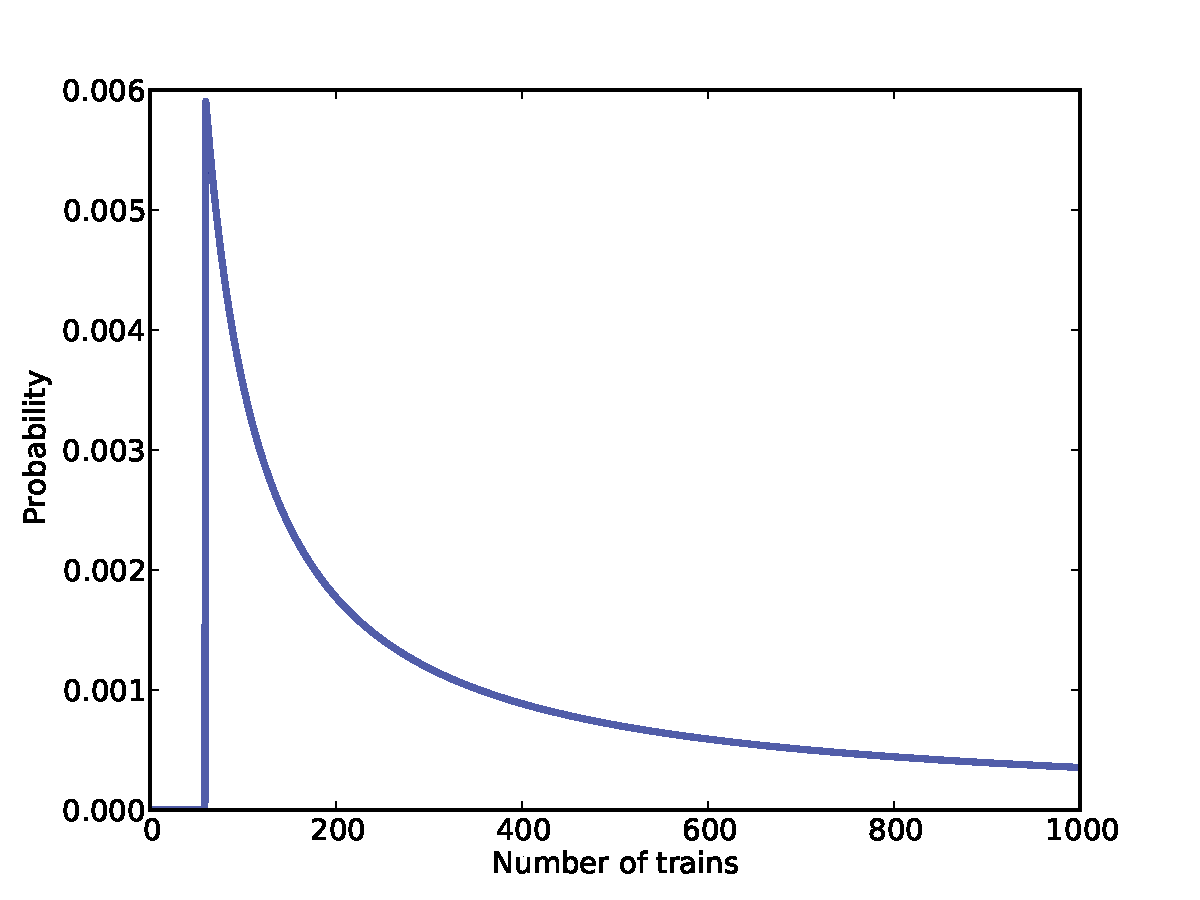
\includegraphics[height=2.5in]{figs/train1.pdf}}
\caption{Posterior distribution for the Locomotive problem, based
on a uniform prior.}
\label{fig.train1}
\end{figure}

We don't have much basis to choose a prior, but we can
start with something simple and
then evaluate some alternatives.  So let's assume that $N$ is less
than 1000, and equally likely to be any value from 1 to 1000.

\begin{verbatim}
    hypos = xrange(1, 1001)
    suite = Train(hypos)
\end{verbatim}

Now all we need is a likelihood function.  With a little thought,
you will realize that the likelihood functions for the Locomotive
problem and the Dice problem are identical:

\begin{verbatim}
class Train(Suite):
    def Likelihood(self, hypo, data):
        if hypo < data:
            return 0
        else:
            return 1.0/hypo
\end{verbatim}

And here's the update:

\begin{verbatim}
    suite.Update(60)
\end{verbatim}

Since there are 1000 hypotheses, I didn't print the results.
Instead I used {\tt myplot.Pmf}:

\begin{verbatim}
    myplot.Pmf(suite)
    myplot.Show(xlabel='Number of trains',
                ylabel='Probability')
\end{verbatim}

The result is in Figure~\ref{fig.train1}.  Not surprisingly, all
values of $N$ below 60 have been eliminated.  The most likely
value, if you had to guess, is 60.  That might not seem like
a very good guess; after all, what are the chances that you just
happened to see the train with the highest number?

Nevertheless, if you want to maximize the chance of getting
the answer exactly right, you should guess 60.  But maybe that's
not the right goal.  One alternative is to compute the
mean of the posterior distribution:

\begin{verbatim}
def Mean(suite): 
    total = 0
    for hypo, prob in suite.Items():
        total += hypo * prob
    return total

print Mean(suite)
\end{verbatim}

Or you could use the very similar method provided by {\tt Pmf}:

\begin{verbatim}
    print suite.Mean()
\end{verbatim}

The mean of this posterior distribution is 333, so that might be a
good guess if you wanted to minimize error.  If you played this
guessing game over and over, using the mean of the posterior as your
estimate would minimize the total squared error over the long run (see
\url{http://en.wikipedia.org/wiki/Minimum_mean_square_error}).

You can download this example from \url{http://thinkbayes.com/train.py}.


\section{What about that prior?}

To make any progress on the Locomotive problem we had to make
some assumptions, and some of them were pretty arbitrary.  In
particular, we chose a uniform prior from 1 to 1000, without
much justification for choosing 1000, or for choosing a uniform
distribution.

It is not crazy to believe that a railroad company might operate
1000 locomotives, but a reasonable person might guess more or fewer.
So we might wonder whether the posterior distribution is sensitive
to these assumptions.  With so little data (only one observation)
it probably is.

Recall that with a uniform prior from 1 to 1000, the mean of
the posterior is 333.  With an upper bound of 500, we get a
posterior mean of 207, and with an upper bound of 2000,
the posterior mean is 552.

So that's bad.  There are two ways to proceed:

\begin{itemize}

\item Get more data.

\item Get more background information.

\end{itemize}

With more data, the posterior distributions based on different
priors tend to converge.  For example, suppose that in addition
to train 60 we also see trains 30 and 90.  We can update the
distribution like this:

\begin{verbatim}
    for data in [60, 30, 90]:
        suite.Update(data)
\end{verbatim}

With these data, the means of the posteriors are

  \begin{tabular}{|l|l|}
  \hline
  Upper & Posterior \\
  Bound & Mean \\
  \hline
  500 & 152 \\
  1000 & 164\\
  2000 & 171\\
  \hline
  \end{tabular}

So the difference between the posteriors is smaller.


\section{An alternative prior}

\begin{figure}
% train.py
\centerline{\includegraphics[height=2.5in]{figs/train4.pdf}}
\caption{Posterior distribution based on a power law prior,
compared to a uniform prior.}
\label{fig.train4}
\end{figure}

If more data are not available, another option is to improve the
priors by gathering more background information.  It is probably
not reasonable to assume that a railroad company with 1000 locomotives
is just as likely as a company with only 1.

With some effort, we could probably find a list of companies that
operate locomotives in the area of observation.  Or we could
interview an expert in rail shipping to gather information about
the typical size of companies.

But even without getting into the specifics of railroad economics, we
can make some educated guesses.  In most fields, there are many small
companies, fewer medium-sized companies, and only one or two very
large companies.  In fact, the distribution of company sizes tends to
follow a power law, as Robert Axtell reports in {\it Science} (see
\url{http://www.sciencemag.org/content/293/5536/1818.full.pdf}).

This law suggests that if there are 1000 companies with fewer than
10 locomotives, there might be 100 companies with 100 locomotives,
10 companies with 1000, and possibly one company with 10,000 locomotives.

Mathematically, a power law means the number of companies
with a given size is inversely proportional to the size, or
%
\[ \PMF(x) \propto \left( \frac{1}{x} \right)^{\alpha}   \]
%
where $\PMF(x)$ is the probability mass function of $x$ and $\alpha$ is
a parameter that is often near 1.

We can construct a power law prior like this:

\begin{verbatim}
class Train(Dice):
    def __init__(self, hypos, alpha=1.0):
        Pmf.__init__(self)
        for hypo in hypos:
            self.Set(hypo, hypo**(-alpha))
        self.Normalize()
\end{verbatim}

And here's the code that constructs the prior:

\begin{verbatim}
    hypos = range(1, 1001)
    suite = Train(hypos)
\end{verbatim}

Again, the upper bound is arbitrary, but with a power law
prior, the posterior is less sensitive to this choice.

Figure~\ref{fig.train4} shows the distribution after
we see train 60, comparing the posterior based on the power
law prior to the posterior based on a uniform prior, both
with upper bound 1000.  Using the additional background
represented in the power law prior, we can all but eliminate
values of $N$ greater than 700.

If we start with this prior and observe trains 30, 60 and 90,
the means of the posteriors are

  \begin{tabular}{|l|l|}
  \hline
  Upper & Posterior \\
  Bound & Mean \\
  \hline
  500 & 131 \\
  1000 & 133 \\
  2000 & 134 \\
  \hline
  \end{tabular}

Now the difference between the posteriors is much smaller.  In fact,
with an arbitrarily large upper bound, the mean converges on 134.

So the power law prior is more realistic, because it is based on
general information about the size of companies, and it
behaves better in practice.

You can download the examples in this section from
\url{http://thinkbayes.com/train3.py}.

\section{Credible intervals}

Once you have computed a posterior distribution, it is often useful
to summarize the results with a single point estimate or an interval.
For point estimates it is common to use the mean, median, or the
value with maximum likelihood.

For intervals we usually report two values computed
so that there is a 90\% chance that the unknown value falls
between them, or 95\%, or some other value.
These values define a ``credible interval.''

A simple way to compute a credible interval is to add up the
probabilities in the posterior distribution and record the values
that correspond to probabilities 5\% and 95\%.  In other words,
the 5th and 95th percentiles.

\verb"thinkbayes" provides a function that computes percentiles:

\begin{verbatim}
def Percentile(pmf, percentage):
    p = percentage / 100.0
    total = 0
    for val, prob in pmf.Items():
        total += prob
        if total >= p:
            return val    
\end{verbatim}

And here's the code that uses it:

\begin{verbatim}
    interval = Percentile(suite, 5), Percentile(suite, 95)
    print interval
\end{verbatim}

For the previous example---the locomotive problem with a power law prior
and three trains---the 90\% credible interval is $(91, 243)$.  The
width of this range suggests, correctly, that we are still quite
uncertain about how many locomotives there are.


\section{Cumulative distribution function}

In the previous section we computed percentiles by iterating through
the values and probabilities in a Pmf.  If we need to compute more
than a few percentiles, it is more efficient to use a cumulative
distribution function, or Cdf.

Cdfs and Pmfs are equivalent in the sense that they contain the
same information about the distribution, and you can always convert
from one to the other.  The advantage of the Cdf is that you can
compute percentiles more efficiently.

{\tt thinkbayes} provides a {\tt Cdf} class that represents a
cumulative distribution function.  It also provides functions for
converting from a Pmf to a Cdf (and back). 

\begin{verbatim}
import thinkbayes
cdf = thinkbayes.MakeCdfFromPmf(suite)
\end{verbatim}

And Cdf provides a function named \verb"Percentile"

\begin{verbatim}
    interval = cdf.Percentile(5), cdf.Percentile(95)
\end{verbatim}

Converting from a Pmf to a Cdf takes time proportional to the number
of values.  The Cdf stores the values and probabilities in sorted
lists, so looking up a probability to get the corresponding value
takes ``log time,'' that is, time proportional to the logarithm of the
number of values.  Looking up a value to get the corresponding
probability is also logarithmic, so Cdfs are efficient for many
calculations.

The examples in this section are in \url{http://thinkbayes.com/train.py}.


\chapter{More estimation}

\section{Four Urns}

James Joyce, the American philosopher not the Irish author, wrote
a paper called {\it How probabilities reflect evidence} that poses
the following problem (which I am quoting loosely):

\begin{quote}
Jacob and Emily both start out knowing that an urn, U, was
randomly chosen from a set of four urns ${urn_0, urn_1, urn_2, urn_3}$
where $urn_i$ contains three balls, $i$ of which are blue and $3-i$ of
which are green. [...]  Jacob and Emily regard random drawing with
replacement as an exchangeable process, so that any series of draws
that produces m blue balls and n green balls is as likely as any other
such series, irrespective of order.  Use $B^m G^n$ to denote the generic
event in which $m$ blue balls and $n$ green balls are drawn at random
and with replacement from U.  Against this backdrop of shared
evidence, suppose Jacob sees five balls drawn at random and with
replacement from U and observes that all are blue, so his evidence is
$B^5 G^0$.  Emily, who sees Jacob's evidence, looks at fifteen additional
draws of which twelve come up blue, so her evidence is $B^{17} G^3$.  [If
$B_{next}$ is the probability that the next ball drawn from the urn is
blue,] what should Emily and Jacob think about $B_{next}$?
\end{quote}

We'll proceed in two steps: the first is to compute the probability
that U is $urn_i$ for each $i$.  The second is to compute $B_{next}$.

Let's use $H_i$ to represent the hypothesis that the urn we chose, U,
is $urn_i$.  Since we are told that U was chosen at random, we can
infer that the prior probabilities are $H_i = 1/4$ for all $i$.

And the likelihood function is easy.  If $H_i$ is true, U contains
$i$ blue balls, so $\p{B|H_i} = i/3$.  Or in Python

\begin{verbatim}
class Urn(Suite):
    def Likelihood(self, hypo, data):
        """
        hypo: integer number of blue balls (out of three)
        data: string 'B' or 'G'
        """
        p = hypo / 3.0
        if data == 'B':
            return p
        else:
            return 1-p
\end{verbatim}

And here's the code that creates the prior and updates it
with Jacob's data:

\begin{verbatim}
    suite = Urn([0,1,2,3])

    for data in 'BBBBB':
        suite.Update(data)
\end{verbatim}

And here are the results:

\begin{verbatim}
0 0.0
1 0.0036231884058
2 0.115942028986
3 0.880434782609
\end{verbatim}

Since he has seen 5 blue and no green balls, Jacob rules out $urn_0$
and gives low posterior probabilities to $urn_1$ and $urn_2$.  Based
on this data, Jacob is 88\% sure that U is $urn_3$.

So what should Jacob believe about $B_{next}$, the chance that the
next ball from U is blue.  If $H_3$ is right, and U is $urn_3$,
then $B_{next}$ is 100\%.  But Jacob is not sure about $H_3$.

Jacob can compute $B_{next}$ using the law of total probability, which
says that the probability that the next ball is blue is the sum
of the probabilities for each way it can happen; in this case
%
\[ B_{next} = \sum_i \frac{i}{3}~\p{H_i | D} \]
%
Pulling out the factor of $1/3$, we have
%
\[ B_{next} = \frac{1}{3} \sum_i i~\p{H_i | D} \]
%
which we recognize as the mean of the posterior distribution
divided by 3.

\begin{verbatim}
print suite.Mean() / 3.0
\end{verbatim}

For Jacob, $B_{next}$ is 0.96.  For Emily, who sees 17 blue and 3 green
balls, the posterior distribution is 

\begin{verbatim}
0 0.0
1 3.05166468308e-05
2 0.999969483353
3 0.0
\end{verbatim}

Since Emily has seen a blue and a green ball, she can rule out $H_0$
and $H_3$.  And since she has seen many more blue than green balls,
she is all but certain that U is $urn_2$, so her value for $B_{next}$
is very close to 2/3.

Joyce constructed this example to point out a difference between the
evidence seen by Jacob and Emily.  Jacob's evidence has more
``force,'' in one sense of the word, because his posterior belief
about $B_{next}$ is more strongly biased.  But Emily's evidence has
more ``weight,'' because she is more confident about which urn U is.

For Joyce the point of this example is to probe what we mean
when we talk about the ``weight'' or ``force,'' of
evidence.  We come back to this question, from a Bayesian
perspective, in the next chapter.

For us, the point of this example is to provide a warm-up exercise
that will help with the next problem.


\section{The Euro coin problem}
\label{euro}

In {\it Information Theory, Inference, and Learning Algorithms}, David MacKay
poses this question:

\begin{quote}
A statistical statement appeared in ``The Guardian" on Friday January 4, 2002:

  \begin{quote}
        When spun on edge 250 times, a Belgian one-euro coin came
        up heads 140 times and tails 110.  `It looks very suspicious
        to me,' said Barry Blight, a statistics lecturer at the London
        School of Economics.  `If the coin were unbiased, the chance of
        getting a result as extreme as that would be less than 7\%.'
        \end{quote}

But do these data give evidence that the coin is biased rather than fair?
\end{quote}

To answer that question, we'll proceed in two steps.  The first
is to estimate the probability that the coin lands face up.  The second
is to evaluate whether the data support the hypothesis that the
coin is biased.

Any given coin has some probability, $x$, of landing heads up when spun
on edge.  It seems reasonable to believe that the value of $x$ depends
on some physical characteristics of the coin, primarily the distribution
of weight.

If a coin is perfectly balanced, we expect $x$ to be close to 50\%, but
for a lop-sided coin $x$ might be substantially different.  We can use
Bayes's Theorem and the observed data to estimate $x$.

Let's define 101 hypotheses, where $H_i$ is the hypothesis that
$x$ is $i$\%, for values of $i$ from 0 to 100.  I'll start with a uniform
prior where the probability of $H_i$ is the same for all $i$.  We'll
come back later to consider other priors.

\begin{figure}
% euro.py
\centerline{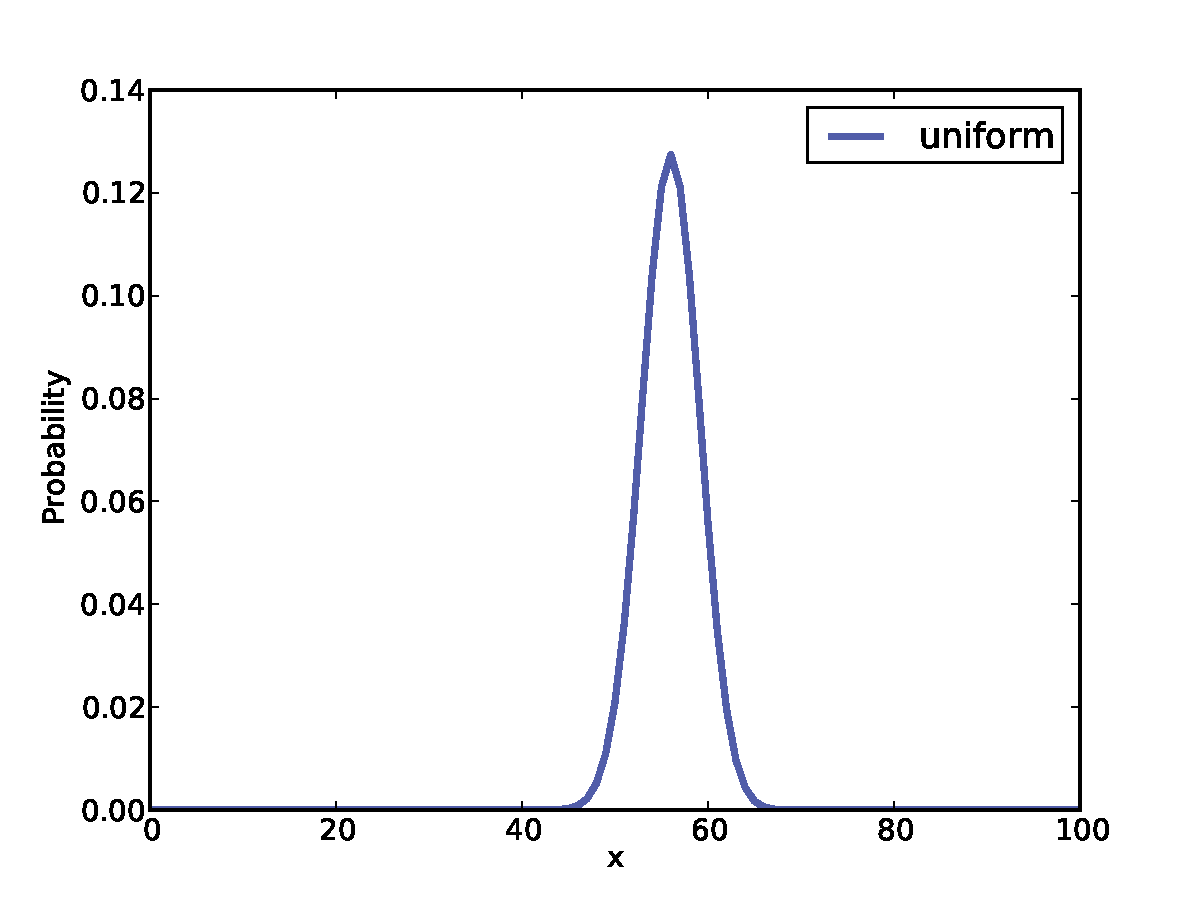
\includegraphics[height=2.5in]{figs/euro1.pdf}}
\caption{Posterior distribution for the Euro problem
on a uniform prior.}
\label{fig.euro1}
\end{figure}

The likelihood function is easy; in fact, it is the same as in
the Four Urn problem.  If $H_i$ is true, then the probability of
heads is $i/100$; the probability of tails is $1- i/100$.

\begin{verbatim}
class Euro(Suite):

    def Likelihood(self, hypo, data):
        x = hypo / 100.0
        if data == 'H':
            return x
        else:
            return 1-x
\end{verbatim}

Here's the code that makes the suite and updates it:

\begin{verbatim}
    suite = Euro(xrange(0, 101))
    dataset = 'H' * 140 + 'T' * 110

    for data in dataset:
        suite.Update(data)
\end{verbatim}

And then we can plot the posterior.

\begin{verbatim}
    myplot.Pmf(suite)
    myplot.Show()
\end{verbatim}

The result is in Figure~\ref{fig.euro1}.


\section{Summarizing the posterior}

Again, there are several ways to summarize the posterior distribution.
One option is to find the most likely value in the posterior
distribution.  \verb"thinkbayes" provides a function that does 
that:

\begin{verbatim}
def MaximumLikelihood(pmf):
    """Returns the value with the highest probability."""
    prob, val = max((prob, val) for val, prob in pmf.Items())
    return val
\end{verbatim}

In this case the result is 56, which is also the observed percentage of
heads, $140/250 = 0.56\%$.  So that suggests (correctly) that the
percentage in a sample is the maximum likelihood estimator
for the population.

We might also summarize the posterior by computing the mean
and median:

\begin{verbatim}
    print 'Mean', suite.Mean()
    print 'Median', thinkbayes.Percentile(suite, 50)
\end{verbatim}

The mean is 55.95; the median is 56.  Finally, we can compute a
credible interval: 

\begin{verbatim}
    print 'CI', thinkbayes.CredibleInterval(suite, 90)
\end{verbatim}

The result is $(51, 61)$.

Now, getting back to the original question,
we would like to know whether the coin is fair.  We observe
that the posterior credible interval does not include 50\%,
which suggests that the coin is not fair.

But that is not exactly the question we started with.  MacKay asked,
`` Do these data give evidence that the coin is biased rather than
fair?''  To answer that question, we will have to be more precise
about what it means to say that data constitute evidence for
a hypothesis.  And that is the subject of the next chapter.

But before we go, I want to address one possible source of confusion.
Since we want to know whether the coin is fair, it might be tempting
to ask for the probability that {\tt x} is 50\%:

\begin{verbatim}
    print suite.Prob(50)
\end{verbatim}

The result is 0.021, but that value is pretty much meaningless.  The
decision to evaluate 101 hypotheses was arbitrary; we could have
divided the range into more or fewer pieces, and if we had, the
probability for any given hypothesis would be greater or less.


\section{Swamping the priors}
\label{triangle}

\begin{figure}
% euro.py
\centerline{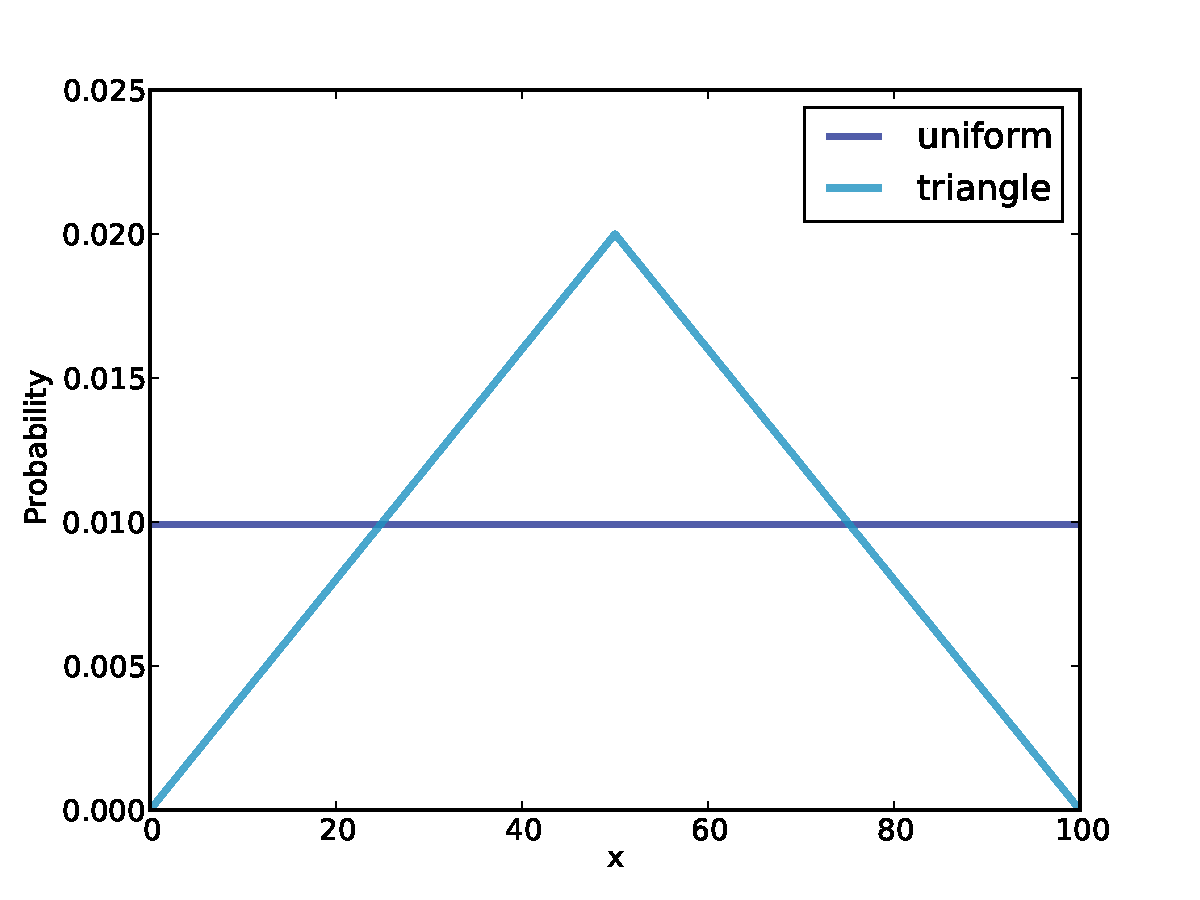
\includegraphics[height=2.5in]{figs/euro2.pdf}}
\caption{Uniform and triangular priors for the
Euro problem.}
\label{fig.euro2}
\end{figure}

\begin{figure}
% euro.py
\centerline{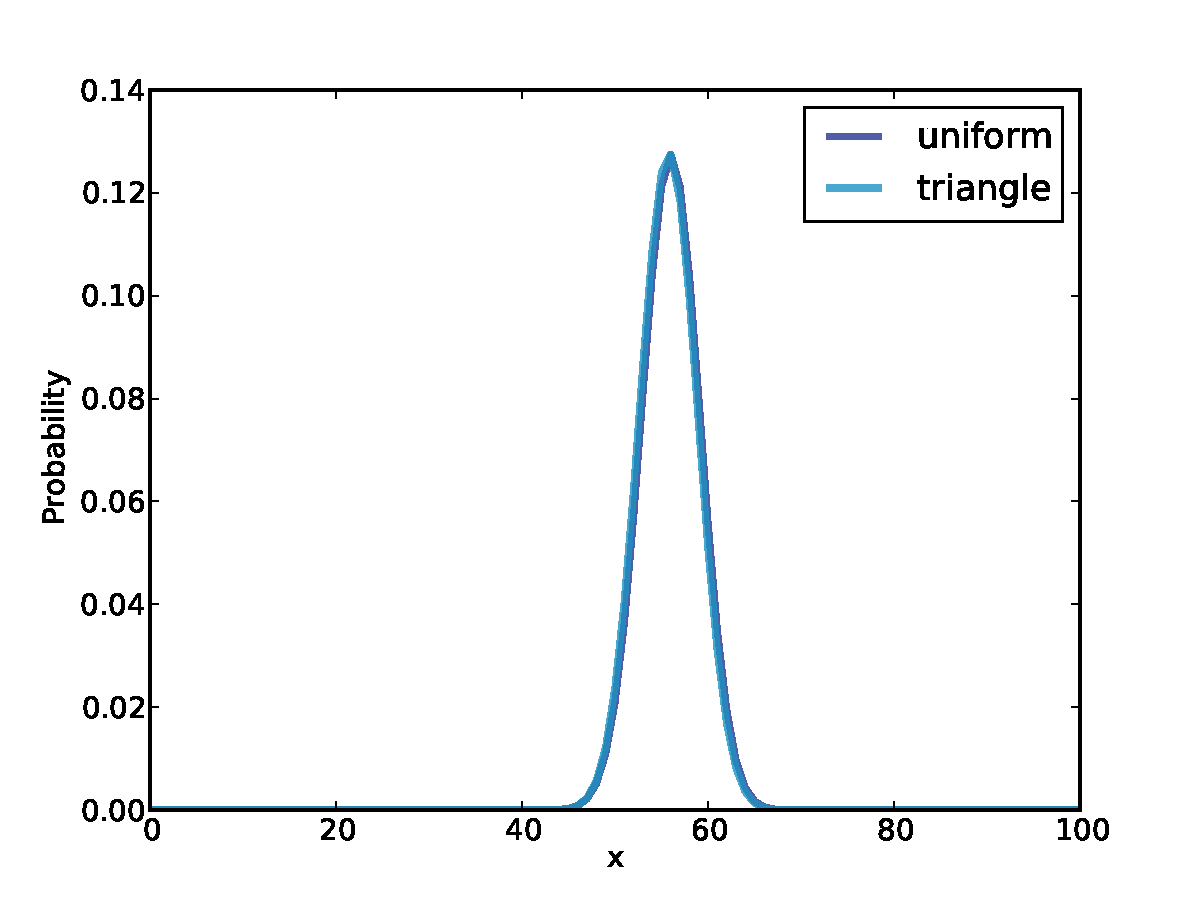
\includegraphics[height=2.5in]{figs/euro3.pdf}}
\caption{Posterior distributions for the Euro problem.}
\label{fig.euro3}
\end{figure}

Again we started with a uniform prior, and again we have to
acknowledge that it was not a very good choice. I can believe
that if a coin is lop-sided, $x$ might deviate substantially from
50\%, but it seems unlikely that the Belgian Euro coin is so
imbalanced that $x$ is 10\% or 90\%.

So it might be more reasonable to choose a prior that gives
higher probability to values of $x$ near 50\% and lower probability
to extreme values.

As an example, I constructed a triangular prior, shown in
Figure~\ref{fig.euro2}.  Here's the code that constructs the prior:

\begin{verbatim}
def TrianglePrior():
    suite = Euro(xrange(0, 101))
    for x in range(0, 51):
        suite.Set(x, x)
    for x in range(51, 101):
        suite.Set(x, 100-x) 
    suite.Normalize()
\end{verbatim}

Figure~\ref{fig.euro2} shows the result.  Updating this prior
with the same dataset yields the posterior distribution shown
in Figure~\ref{fig.euro3}.

The point of this example is that even with substantially different
priors, the posterior distributions are very similar.  The medians
and the credible intervals are identical; the means differ by
less than 0.5\%.

This is an example of ``swamping the priors:'' with enough
data, people who start with different priors will tend to
converge on the same posterior.


\section{Optimization}
\label{optimization}

The code I have shown so far is meant to be easy to read, but it
is not very efficient.  In general, I like to develop code that
is demonstrably correct, then check whether it is fast enough for
my purposes.  If so, there is no need to optimize.
For this example, if we care about run time,
there are several ways we can speed it up.

The first opportunity is to reduce the number of times we
normalize the suite.
In the original code, we call \verb"Update" once for each spin.

\begin{verbatim}
    dataset = 'H' * heads + 'T' * tails

    for data in dataset:
        suite.Update(data)
\end{verbatim}

And here's what \verb"Update" looks like:

\begin{verbatim}
    def Update(self, data):
        for hypo in self.Values():
            like = self.Likelihood(hypo, data)
            self.Mult(hypo, like)
        return self.Normalize()
\end{verbatim}

Each update iterates through the hypotheses, then calls \verb"Normalize",
which iterates through the hypotheses again.  We can save some
time by doing all of the updates before normalizing.

\verb"Suite" provides a method called \verb"UpdateSet" that does
exactly that.  Here it is:

\begin{verbatim}
    def UpdateSet(self, dataset):
        for data in dataset:
            for hypo in self.Values():
                like = self.Likelihood(hypo, data)
                self.Mult(hypo, like)
        return self.Normalize()
\end{verbatim}

And here's how we can invoke it:

\begin{verbatim}
    dataset = 'H' * heads + 'T' * tails
    suite.UpdateSet(dataset)
\end{verbatim}

This optimization speeds things up, but the run time is still
proportional to the amount of data.  We can speed things up
even more by rewriting \verb"Likelihood" to process the entire
dataset, rather than one spin at a time.

In the original version,
\verb"data" is a string that encodes either heads or tails:

\begin{verbatim}
    def Likelihood(self, hypo, data):
        x = hypo / 100.0
        if data == 'H':
            return x
        else:
            return 1-x
\end{verbatim}

As an alternative, we could encode the dataset as a tuple of 
two integers: the number of heads and tails.
In that case \verb"Likelihood" looks like this:

\begin{verbatim}
    def Likelihood(self, hypo, data):
        x = hypo / 100.0
        heads, tails = data
        like = x**heads * (1-x)**tails
        return like
\end{verbatim}

And then we can call \verb"Update" like this:

\begin{verbatim}
    heads, tails = 140, 110
    suite.Update((heads, tails))
\end{verbatim}

Since we have replaced repeated multiplication with exponentiation,
this version takes the same time for any number of spins.


\section{The beta distribution}
\label{beta}

There is one more optimization that solves this problem
even faster.

So far we have used a Pmf object to represent a discrete set of
possible values for {\tt x}.  Now we will use a continuous
distribution, specifically the beta distribution (see
\url{http://en.wikipedia.org/wiki/Beta_distribution}).

The beta distribution is defined on the interval from 0 to 1
(including both), so it is a natural choice for describing
proportions and probabilities.  But wait, it gets better.

It turns out that if you do a Bayesian update with a binomial
likelihood function, as we did in the previous section, the beta
distribution is a ``conjugate prior.''  That means that if the prior
distribution for {\tt x} is a beta distribution, the posterior is also
a beta distribution.  But wait, it gets even better.

The shape of the beta distribution depends on two parameters, written
$\alpha$ and $\beta$, or {\tt alpha} and {\tt beta}.  If the prior
is a beta distribution with parameters {\tt alpha} and {\tt beta}, and
we see data with {\tt h} heads and {\tt t} tails, the posterior is a
beta distribution with parameters {\tt alpha+h} and {\tt beta+t}.  In
other words, we can do an update with two additions.

So that's great, but it only works if the prior is beta.  If beta
distributions were unrealistic priors, they would not be very useful.
But for many realistic priors there is a beta distribution that is at
least a good approximation, and for a uniform prior there is a perfect
match.  The beta distribution with {\tt alpha=1} and {\tt beta=1} is
uniform from 0 to 1.

Let's see how we can take advantage of all this.  Here's
a class that represents a beta distribution:

\begin{verbatim}
class Beta(object):

    def __init__(self, alpha=1, beta=1):
        self.alpha = alpha
        self.beta = beta
\end{verbatim}

By default \verb"__init__" makes a uniform distribution.
{\tt Update} performs a Bayesian update:

\begin{verbatim}
    def Update(self, data):
        heads, tails = data
        self.alpha += heads
        self.beta += tails
\end{verbatim}

{\tt data} is a pair of integers representing the number of
heads and tails, or in the language of Bernoulli trials: successes
and failures.

The mean of a beta distribution is a simple function of {\tt alpha}
and {\tt beta}:

\begin{verbatim}
    def Mean(self):
        return float(self.alpha) / (self.alpha + self.beta)
\end{verbatim}

So we have yet another way to solve the Euro problem:

\begin{verbatim}
    beta = Beta()
    beta.Update((140, 110))
    print beta.Mean()
\end{verbatim}

The posterior mean is 56\% (again).  To get the probability for
any value of {\tt x}, we can evaluate the PDF of the beta
distribution:

\begin{verbatim}
    def EvalPdf(self, x):
        return x**(self.alpha-1) * (1-x)**(self.beta-1)
\end{verbatim}

This expression might look familiar.  Here's {\tt
  thinkbayes.EvalBinomialPmf}

\begin{verbatim}
def EvalBinomialPmf(x, yes, no): 
    return x**yes * (1-x)**no
\end{verbatim}

It's the same function, but in {\tt EvalPdf}, we think of {\tt x} as a
random variable and {\tt alpha} and {\tt beta} as parameters; in {\tt
  EvalBinomialPmf}, {\tt x} is the parameter, and {\tt yes} and {\tt
  no} are random variables.  Distributions like these that share the
same PDF are called ``conjugate distributions.''

{\tt Beta} is defined in \url{http://thinkbayes.com/thinkbayes.py}.


\section{Exercises}

\begin{exercise}

Suppose that instead of observing coin tosses directly, you measure
the outcome using an instrument that is not always correct.  Specifically,
suppose there is a probability {\tt y} that an actual heads is reported
as tails, or actual tails reported as heads.

Write a class that estimates the bias of a coin given a series of
outcomes and the value of {\tt y}.

How does the spread of the posterior distribution depend on
{\tt y}?

\end{exercise}


\begin{exercise}

This exercise is inspired by a question posted by a
``redditor'' named dominosci on Reddit's statistics ``subreddit'' at
\url{http://reddit.com/r/statistics}.

Reddit is an online forum with many interest groups called
subreddits.  Users, called redditors, post links to online
content and other web pages.  Other redditors vote on the links,
giving an ``upvote'' to high-quality links and a ``downvote'' to
links that are bad or irrelevant.

A problem, identified by dominosci, is that some redditors
are more reliable than others, and Reddit does not currently take
this into account.

So the challenge is to devise a system so that when a redditor
casts a vote, the estimated quality of the link is updated
in accordance with the reliability of the redditor, and the
estimated reliability of the redditor is updated in accordance
with the quality of the link.

One approach is to model the quality of the link as the
probability of garnering an upvote, and to model the reliability
of the redditor as the probability of correctly giving an upvote
to a high-quality item.

Write class definitions for redditors and links and an update function
that updates both objects whenever a redditor casts a vote.

\end{exercise}


\chapter{Odds and addends}

\section{Odds}

One way to represent a probability is with a number between
0 and 1, but that's not the only way.  If you have ever bet
on a football game or a horse race, you have probably encountered
another representation of probability, called ``odds.''

You might have heard expressions like ``the odds are
three to one against,'' but you might not know what they mean.  
The odds in favor of an event are the ratio of the probability
it will occur to the probability that it will not.

So if I think my team has a 75\% chance of winning, I would
say that the odds in their favor are three to one, because
the chance of winning is three times the chance of losing.

You can write odds in decimal form, but it is most common to
write them as a ratio of integers.  So ``three to one'' is
written $3:1$.

When probabilities are low, it is more common to report the
``odds against'' rather than the odds in favor.  For
example, if I think my horse has a 10\% chance of winning,
I would say that the odds against are $9:1$.

Probabilities and odds are different representations of the
same information.  Given a probability, you can compute the
odds like this:

\begin{verbatim}
def Odds(p):
    return p / (1-p)
\end{verbatim}

Given the odds in favor, in decimal form, you can convert to
probability like this:

\begin{verbatim}
def Probability(o):
    return o / (o+1)
\end{verbatim}

If you represent odds with a numerator and denominator, you
can convert to probability like this:

\begin{verbatim}
def Probability2(yes, no):
    return yes / (yes + no)
\end{verbatim}

When I work with odds in my head, I find it helpful to picture
people at the track.  If 20\% of them think my horse will win,
then 80\% of them don't, so the odds in favor are $20:80$ or
$1:4$.

If the odds are $5:1$ against my horse, then five out of six
people think she will lose, so the probability of winning
is $1/6$.

\section{The odds form of Bayes's Theorem}

In Chapter~\ref{intro} I wrote Bayes's Theorem in the ``probability
form'':
%
\[ \p{H|D} = \frac{\p{H}~\p{D|H}}{\p{D}} \]
%
If we define $\bar{H}$ as ``hypothesis H is false'', we can write the
odds in favor of $H$ like this:
%
\[ \frac{\p{H|D}}{\p{\bar{H}|D}} = \frac{\p{H}~\p{D|H}}
                                        {\p{\bar{H}}~\p{D|\bar{H}}} \]
%
Or writing \o{H} for odds in favor of H:
%
\[ \o{H|D} = \o{H} \frac{\p{D|H}}{\p{D|\bar{H}}} \]
%
In words, this says that the posterior odds are the prior odds times
the likelihood ratio.  This is the ``odds form'' of Bayes's Theorem.

This form is most convenient for computing a Bayesian update on
paper, or in your head.  For example, let's go back to the
cookie problem:

\begin{quote}
Suppose there are two bowls of cookies.  Bowl 1 contains
  30 vanilla cookies and 10 chocolate cookies.  Bowl 2 contains 20 of
  each.

Now suppose you choose one of the bowls at random and, without looking,
select a cookie at random.  The cookie is vanilla.  What is the probability
that it came from Bowl 1?
\end{quote}

The prior probability is 50\%, so the prior odds are $1:1$, or just
$1$.  The likelihood ratio is $\frac{3}{4} / \frac{1}{2}$, or $3/2$.
So the posterior odds are $3:2$, which corresponds to probability
$3/5$.


\section{Oliver's blood}
\label{oliver}

Here is another problem from MacKay's {\it Information Theory,
  Inference, and Learning Algorithms}:

\begin{quote}
Two people have left traces of their own blood at the scene of
a crime.  A suspect, Oliver, is tested and found to have type
'O' blood.  The blood groups of the two traces are found to
be of type 'O' (a common type in the local population, having frequency
60\%) and of type 'AB' (a rare type, with frequency 1\%).
Do these data [the traces found at the scene] give evidence
in favor of the proposition that Oliver was one of the people
[who left blood at the scene]?
\end{quote}

To answer this question, we need to think about what it means
for data to give evidence in favor of (or against) a hypothesis.
Intuitively, we might say that data favor a hypothesis if the
hypothesis is more likely in light of the data than it was before.

In the cookie problem, the prior odds are $1:1$, or probability 50\%.
The posterior odds are $3:2$, or probability 60\%.  So we could say
that the vanilla cookie is evidence in favor of Bowl 1.

The odds form of Bayes's Theorem provides a way to make this
intuition more precise.  Again
%
\[ \o{H|D} = \o{H} \frac{\p{D|H}}{\p{D|\bar{H}}} \]
%
Or dividing through by \o{H}:
%
\[ \frac{\o{H|D}}{\o{H}} = \frac{\p{D|H}}{\p{D|\bar{H}}} \]
%
The term on the left is the ratio of the posterior and prior odds.
The term on the right is the likelihood ratio, also called the ``Bayes
factor''.

If the Bayes factor value is greater than $1$, that means that the
data were more likely under $H$ than under $\bar{H}$.  And since the
odds ratio is also greater than $1$, that means that the odds are
greater, in light of the data, than they were before.

If the Bayes factor is less than $1$, that means the data were
less likely under $H$ than under $\bar{H}$, so the odds in
favor of $H$ go down.

Finally, if the Bayes factor is exactly $1$, the data are equally
likely under either hypothesis, so the odds do not change.

Now we can get back to the Oliver's blood problem.  If Oliver is
one of the people who left blood at the crime scene, then he
accounts for the 'O' sample, so the probability of the data
is just the probability that a random member of the population
has type 'AB' blood, which is 1\%.

If Oliver did not leave blood at the scene, then we have two
samples to account for.  If we choose two random people from
the population, what is the chance of finding one with type 'O'
and one with type 'AB'?  Well, there are two ways it might happen:
the first person we choose might have type 'O' and the second
'AB', or the other way around.  So the total probability is
$2 (0.6) (0.01)\ = 1.2\%$.

The likelihood of the data is slightly higher if Oliver is
{\it not} one of the people who left blood at the scene, so
the blood data is actually evidence against Oliver's guilt.

This example is a little contrived, but it is an example of
the counterintuitive result that data {\it consistent} with
a hypothesis are not necessarily {\it in favor of}
the hypothesis.

If this result is so counterintuitive that it bothers you,
this way of thinking might help: the data consist of a common
event, type 'O' blood, and a rare event, type 'AB' blood.
If Oliver accounts for the common event, that leaves the rare
event still unexplained.  If Oliver doesn't account for the
'O' blood, then we have two chances to find someone in the
population with 'AB' blood.  And that factor of two makes
the difference.

\section{Addends}
\label{addends}

Dungeons and Dragons is a role-playing game where the results
of players' decisions are usually determined by rolling dice.
In fact, before game play starts, players generate each
attribute of their characters---strength, intelligence, wisdom,
dexterity, constitution, and charisma---by rolling three
six-sided dice and adding them up.

So you might be curious to know the distribution of this sum.
There are two ways you might compute it:

\begin{description}

\item[Simulation:] Given a Pmf that represents the distribution
for a single die, you can draw random samples, add them up,
and accumulate the distribution of simulated sums.

\item[Enumeration:] Given two Pmfs, you can enumerate all possible
pairs of values and compute the distribution of the sums.

\end{description}

\verb"thinkbayes" provides functions for both.  Here's an example
of the first approach.  First, I'll define a class to represent
a single die as a Pmf:

\begin{verbatim}
class Die(thinkbayes.Pmf):
    def __init__(self, sides):
        d = dict((i, 1) for i in xrange(1, sides+1))
        thinkbayes.Pmf.__init__(self, d)
        self.Normalize()
\end{verbatim}

Now I can create a six-sided die:

\begin{verbatim}
    d6 = Die(6)
\end{verbatim}

And use \verb"SampleSum" to generate a sample of 1000 rolls.

\begin{verbatim}
    dice = [d6] * 3
    three = thinkbayes.SampleSum(dice, 1000)
\end{verbatim}

\verb"SampleSum" is based on another function, \verb"RandomSum",
also in \verb"thinkbayes.py":

\begin{verbatim}
def RandomSum(dists):
    total = sum(dist.Random() for dist in dists)
    return total


def SampleSum(dists, n):
    pmf = MakePmfFromList(RandomSum(dists) for i in xrange(n))
    return pmf
\end{verbatim}

\verb"dists" is a list of objects that can be either
Pmfs or Cdfs (or anything else that provides an appropriate
\verb"Random" method); \verb"n" is the number of rolls to simulate.

The drawback of estimating this distribution by simulation is that
it is only approximately correct.  As \verb"n" gets larger, it gets
more accurate, but of course the run time increases as well.

The other approach is to enumerate all pairs of values and
compute the sum and probability of each pair.  This is implemented
in the \verb"Pmf.__add__" method:

\begin{verbatim}
    def __add__(self, other):
        pmf = Pmf()
        for v1, p1 in self.Items():
            for v2, p2 in other.Items():
                pmf.Incr(v1+v2, p1*p2)
        return pmf
\end{verbatim}

And here's how it's used:

\begin{verbatim}
    three_exact = d6 + d6 + d6
\end{verbatim}

The approximate and exact distributions are shown in
Figure~\ref{fig.dungeons1}.

\begin{figure}
% dungeons.py
\centerline{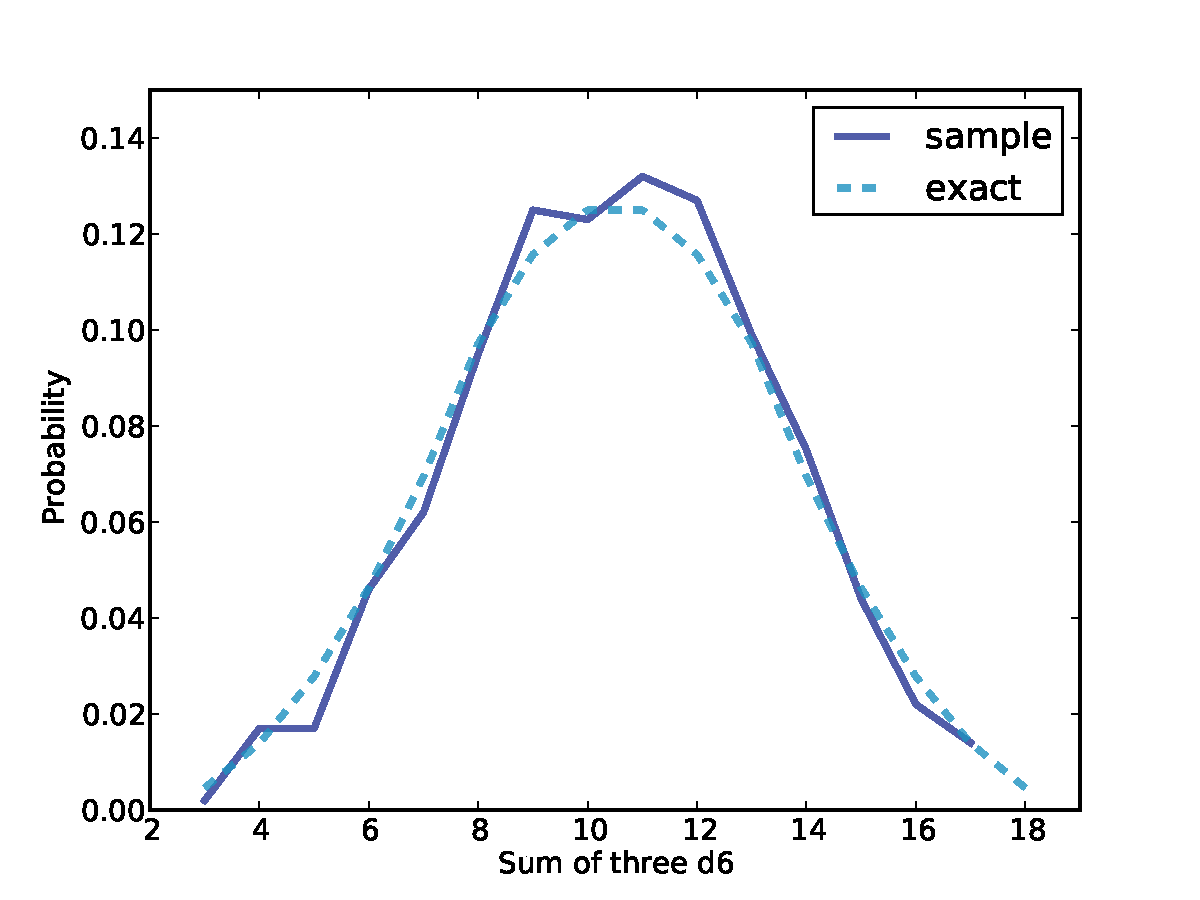
\includegraphics[height=2.5in]{figs/dungeons1.pdf}}
\caption{Approximate and exact distributions for the sum of
three six-sided dice.}
\label{fig.dungeons1}
\end{figure}

\verb"Pmf.__add__" is based on the assumption that the random
selections from each Pmf are independent.  In the example of rolling
several dice, this assumption is pretty good.  In other cases, we
might have to extend this method to use conditional probabilities.

The code from this section is available from
\url{http://thinkbayes.com/dungeons.py}.


\section{Maxima}

\begin{figure}
% dungeons.py
\centerline{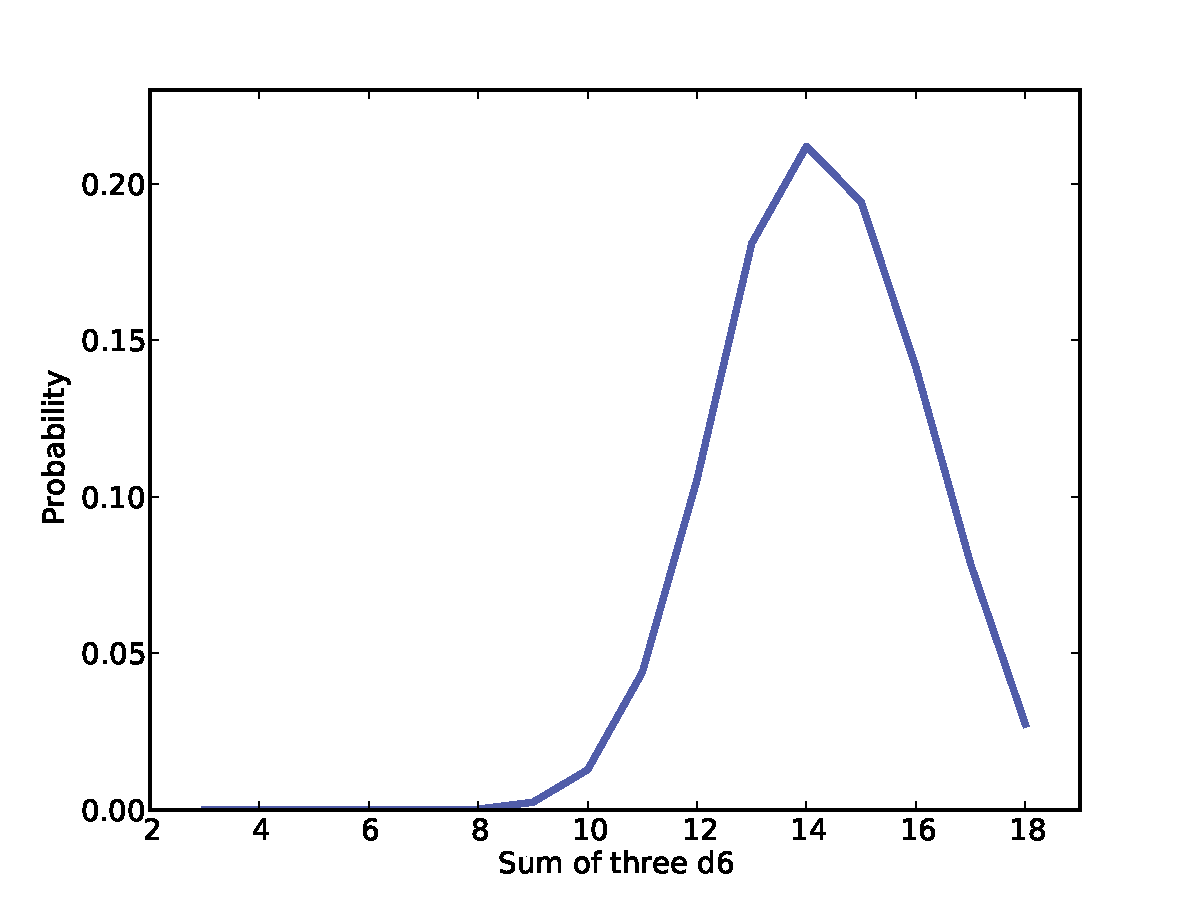
\includegraphics[height=2.5in]{figs/dungeons2.pdf}}
\caption{Distribution of the maximum of six rolls of three dice.}
\label{fig.dungeons2}
\end{figure}

Having generated a Dungeons and Dragons character, I would be
particularly interested in the character's best attributes, so
I might wonder what is the chance of getting an 18 in one or
more attributes, or more generally what is the
distribution of the best attribute.

There are three ways to compute the distribution of a maximum:

\begin{description}

\item[Simulation:] Given a Pmf that represents the distribution
for a single selection, you can a random samples, find the maximum,
and accumulate the distribution of simulated maxima.

\item[Enumeration:] Given two Pmfs, you can enumerate all possible
pairs of values and compute the distribution of the maxima.

\item[Exponentiation:] If we convert a Pmf to a Cdf, there is a simple
and efficient algorithm for finding the Cdf of the maxima.

\end{description}

The code to simulate maxima is almost identical to the code for
simulating sums:

\begin{verbatim}
def RandomMax(dists):
    total = max(dist.Random() for dist in dists)
    return total


def SampleMax(dists, n):
    pmf = MakePmfFromList(RandomMax(dists) for i in xrange(n))
    return pmf
\end{verbatim}

All I did was replace ``sum'' with ``max''.  And the code
for enumeration is almost identical, too:

\begin{verbatim}
def PmfMax(pmf1, pmf2):
    res = thinkbayes.Pmf()
    for v1, p1 in pmf1.Items():
        for v2, p2 in pmf2.Items():
            res.Incr(max(v1, v2), p1*p2)
    return res
\end{verbatim}

In fact, you could generalize this function by taking the
appropriate operator as a parameter.

The only problem with this algorithm is that if each Pmf
has $n$ values, the run time is proportional to $n^2$.

If we convert the Pmfs to Cdfs, we can do the same calculation
in linear time!  The key is to remember the definition of the
cumulative distribution function:
%
\[ CDF(x) = \p{X \le x} \]
%
where $X$ is a random variable that means ``a value chosen
randomly from this distribution.''  So, for example, $CDF(5)$
is the probability that a value from this distribution is less
than or equal to 5.

If I draw $X$ from $CDF_1$ and $Y$ from $CDF_2$, and compute
the maximum $Z = max(X, Y)$, what is the chance that $Z$ is
less than or equal to 5?  Well, in that case both $X$ and $Y$
must be less than or equal to 5.

If the selections of $X$ and $Y$ are independent,
%
\[ CDF_3(5) = CDF_1(5) CDF_2(5) \] 
%
where $CDF_3$ is the distribution of $Z$.  I chose the value
5 because I think it makes the formulas easy to read, but we
can generalize for any value of $z$:
%
\[ CDF_3(z) = CDF_1(z) CDF_2(z) \]
%
In the special case where we draw $n$ values from the same
distribution, 
%
\[ CDF_n(z) = CDF_1(z)^n \]
%
And \verb"Cdf" provides a method that does just that:

\begin{verbatim}
    def Max(self, n):
        cdf = self.Copy()
        cdf.ps = [p**n for p in cdf.ps]
        return cdf
\end{verbatim}

\verb"Max" takes the sample size, {\tt n}, and returns a new
Cdf that represents the distribution of the maximum of {\tt n}
values.

\verb"Pmf.Max" does the same thing for Pmfs.  It has to
do a little more work to convert the Pmf to a Cdf, so the
run time is proportional to $n \log n$, but that's still
better than quadratic.

Finally, here's an example that computes the distribution of
your character's best attribute:

\begin{verbatim}
    best_attr_cdf = three_exact.Max(6)
    best_attr_pmf = thinkbayes.MakePmfFromCdf(best_attr_cdf)
\end{verbatim}

Where \verb"three_exact" is defined in the previous section.
If we print the results, we see that the chance of generating
a character with at least one attribute of 18 is about 3\%.
Figure~\ref{fig.dungeons2} shows the distribution.


\chapter{Optimization}
\label{optimization}

\section{The Price is Right problem}

On November 1, 2007, contestants named Letia and Nathaniel appeared
on The Price is Right, an American game show.  They competed in
a game called the Showcase, where the objective is to guess the price
of a showcase of prizes.  The contestant who comes closest to the
actual price of the showcase, without going over, wins the prizes.

Nathaniel went first.  His showcase included a dishwasher, a wine
cabinet, a laptop computer, and a car.  He bid \$26,000.

Letia's showcase included a pinball machine, a video arcade game, a
pool table, and a cruise of the Bahamas.  She bid \$21,500.

The actual price of Nathaniel's showcase was \$25,347.  He went
over, so he lost.

The actual price of Letia's showcase was \$21,578.  She was only
off by \$78, so she won her showcase and, because
her bid was off by less than \$250, she also won Nathaniel's
showcase.

For a Bayesian thinker, this scenario suggests several questions:

\begin{enumerate}

\item Before seeing the prizes, what prior beliefs should the
  contestant have about the price of the showcase?

\item After seeing the prizes, how should the contestant update
  the prior distribution?

\item Based on the posterior distribution, what should the
  contestant bid?

\end{enumerate}

This problem is inspired by an example in Cameron Davidson-Pilon's
book, {\it Bayesian Methods for Hackers}.


\section{The prior}

To choose a prior distribution of prices, we can take advantage
of data from previous episodes.  Fortunately, fans of the show
keep detailed records.  When I corresponded with Cameron Davidson-Pilon
about his book, he sent me data collected by Steve Gee at
\url{http://tpirsummaries.8m.com}.  It includes the price of
each showcase from the 2011 and 2012 seasons, and the bids
offered by the contestants.

\begin{figure}
% price.py
\centerline{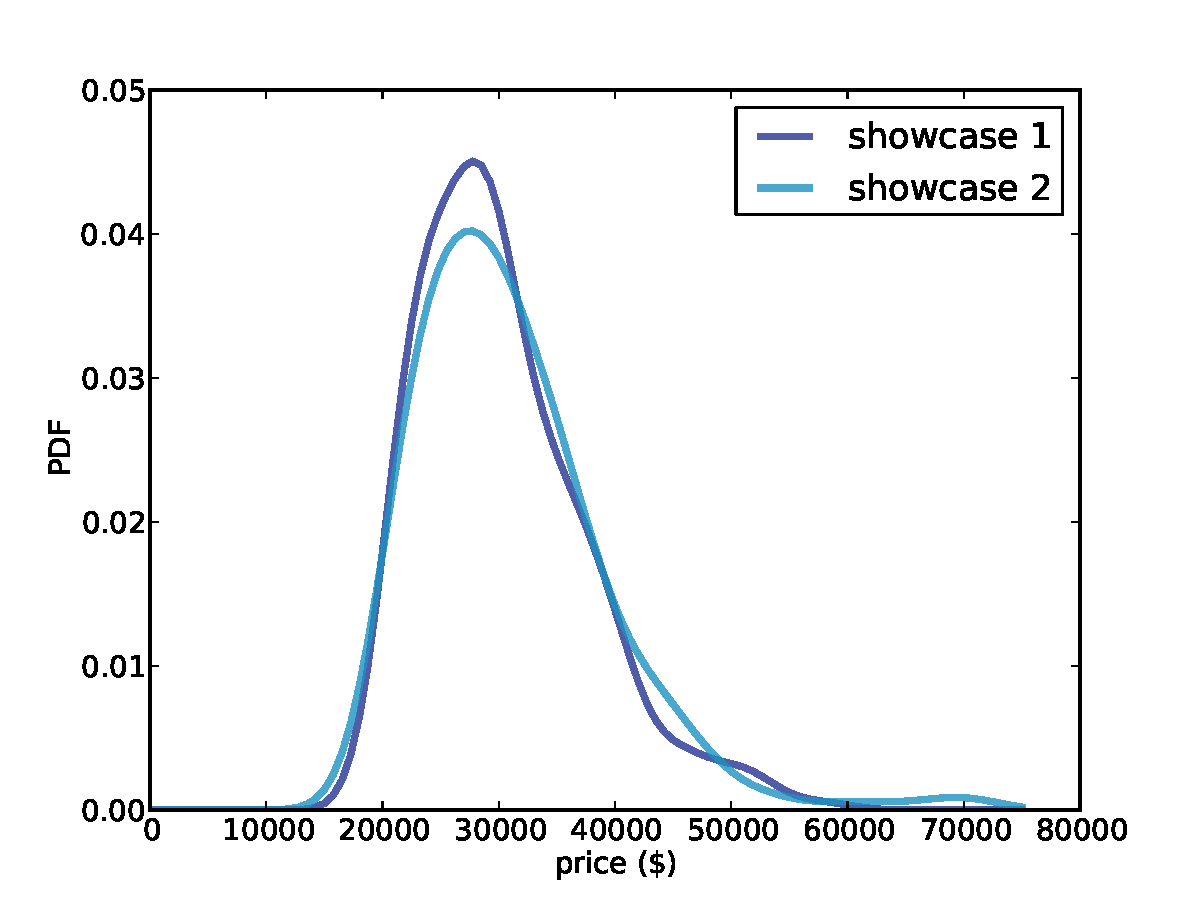
\includegraphics[height=2.5in]{figs/price1.pdf}}
\caption{Distribution of prices for showcases on
{\it The Price is Right}, 2011-12.}
\label{fig.price1}
\end{figure}

Figure~\ref{fig.price1} shows the distribution of prices for these
showcases.  The most common value for both showcases is around
\$28,000, but the first showcase has a second mode near \$50,000,
and the second showcase is occasionally worth more than \$70,000.

These distributions are based on the collected data, but they
have been smoothed by Gaussian kernel density estimation, or KDE.
So before we go on, I want to take a detour to talk about 
probability density functions.


\chapter{PDF}

So far we have been working with probability mass functions,
or Pmfs.  A Pmf is a map from each possible value to its
probability.  In my implementation, a Pmf object provides
a method named {\tt Prob} that takes a value and returns
a probability.

A probability density function, or Pdf, is the continuous version of a
Pmf, where the possible values make up a continuous range rather than
a discrete set.

In mathematical notation, Pdfs are usually written as functions; for
example, here is the Pdf of a Gaussian distribution with
mean 0 and standard deviation 1:

\[ f(x) = \exp(-x^2) \]

To represent a Pdf in Python, I am going to define a new class.
For example, to represent this Gaussian distribution, I might
define:

\begin{verbatim}
class StandardGaussianPdf(object):

    def Density(self, x):
        return math.exp(-x**2)
\end{verbatim}



{\tt Density} takes a value, {\tt x}, and returns the probability
density evaluated at {\tt x}.  A probability density is similar
to a probability in one way: higher density indicates that a
value is more likely.

But it is not a probability.  In order to get a probability, you
have to integrate a density over a range.  But we're not going to
do that.


{\tt thinkbayes.py} provides a class named Pdf that represents
a probability density function.  Here is the definition:

\begin{verbatim}
class Pdf(object):

    def Density(self, x):
        raise UnimplementedMethodException()
\end{verbatim}



\begin{verbatim}
\end{verbatim}


\begin{verbatim}
\end{verbatim}


\begin{verbatim}
\end{verbatim}



\chapter{Prediction}
\label{prediction}

\section{The Boston Bruins problem}

In the 2010-11 National Hockey League (NHL) Finals, my beloved Boston
Bruins played a best-of-seven championship series against the despised
Vancouver Canucks.  Boston lost the first two games 0-1 and 2-3, then
won the next two games 8-1 and 4-0.  At this point in the series, what
is the probability that Boston will win the next game, and what is
their probability of winning the championship?

As always, to answer a question like this, we need to make some
assumptions.  First, it is reasonable to believe that goal scoring in
hockey is at least approximately a Poisson process, which means that
it is equally likely for a goal to be scored at any time during a
game.  Second, we can assume that when team A plays team B, each team
has some long-term average goals per game, denoted $\lambda$.

Given these assumptions, my strategy for answering this question is

\begin{enumerate}

\item Use statistics from previous games to choose a prior
distribution for $\lambda$.

\item Use the score from the first four games to estimate $\lambda$
for each team.

\item Use the posterior distributions of $\lambda$ to compute 
distribution of goals for each team, the distribution of the
goal differential, and the probability that each team wins.

\item Simulate the rest of the series to estimate the probability
of each possible outcome.

\end{enumerate}

To choose a prior distribution, I got some statistics from
\url{http://www.nhl.com}, specifically the average goals per game
for each team in the 2010-11 season.  The distribution is roughly
normal (Gaussian) with mean 2.8 and standard deviation 0.3.

The Gaussian distribution is continuous, but we'll approximate it with
a discrete Pmf.  \verb"thinkbayes" provides \verb"MakeGaussianPmf" to
do exactly that:

\begin{verbatim}
def MakeGaussianPmf(mu, sigma, num_sigmas, n=101):
    pmf = Pmf()
    low = mu - num_sigmas*sigma
    high = mu + num_sigmas*sigma

    for x in numpy.linspace(low, high, n):
        p = EvalGaussianPdf(mu, sigma, x)
        pmf.Set(x, p)
    pmf.Normalize()
    return pmf
\end{verbatim}  

{\tt mu} and {\tt sigma} are the mean and standard deviation of the
Gaussian distribution.  \verb"num_sigmas" is the number of standard
deviations above and below the mean that the Pmf will span, and {\tt
  n} is the number of values in the Pmf.

This is our first use of {\tt numpy}.  {\tt linspace} stands for
``linear space.''  It takes a range, {\tt low} and {\tt high}, and
the number of points, {\tt n}, and returns a new {\tt numpy}
array with {\tt n} elements equally spaced between {\tt low} and
{\tt high}, including both.

\verb"EvalGaussianPdf" does what it says; it evaluates the
Gaussian probability density function (PDF).

\begin{verbatim}
def EvalGaussianPdf(mu, sigma, x):
    z = (x - mu) / sigma
    p = math.exp(-z**2/2)
    return p
\end{verbatim}  

If you look up the Gaussian PDF, you'll see that I left out a
normalizing constant, so this function actually computes
a likelihood that is proportional to the Gaussian PDF.  But
that's fine, because I have to normalize the Pmf anyway.

Getting back to the hockey problem, here's the definition for a suite
of hypotheses about the value of $\lambda$.

\begin{verbatim}
class Hockey(thinkbayes.Suite):

    def __init__(self):
        thinkbayes.Suite.__init__(self)

        pmf = thinkbayes.MakeGaussianPmf(2.7, 0.3, 6)
        for x, p in pmf.Items():
            self.Set(x, p)
\end{verbatim}  

So the prior distribution is Gaussian with mean 2.7, standard deviation
0.3, and it spans six sigmas above and below the mean.

As always, we have to decide how to represent each hypothesis; in
this case I represent the hypothesis that $\lambda=x$ with the
floating-point value {\tt x}. 


\section{Poisson processes}

In mathematical statistics, a ``process'' is a stochastic, or random,
model of a physical system.  For example, a Bernoulli process is a model
of a sequence of events, called trials, in which each trial has
two possible outcomes, like success and failure.  So a Bernoulli
process is a natural model for a series of coin flips, or a series
of shots on goal.

A Poisson process is the continuous version of a Bernoulli process,
where an event can occur at any point in time with equal probability.
Poisson processes can be used to model customers arriving in a store,
buses arriving at a bus stop, or goals scored in a hockey game.

In many real systems the probability of an event changes over time.
Customers are more likely to go to a store at certain times of day,
buses are supposed to arrive at fixed intervals, and goals are more
or less likely at different times during a game.

But all models are based on simplifications, and in this case modeling
a hockey game with a Poisson process is a reasonable choice.  Heuer
et al.~analyze scoring in a German soccer league and come to the same
conclusion; see
\url{http://www.cimat.mx/Eventos/vpec10/img/poisson.pdf}.

The benefit of using this model is that we can compute the distribution
of goals per game efficiently, as well as the distribution of time
between goals.  Specifically, if the average number of goals
in a game is {\tt lam}, the distribution of goals per game is
given by the Poisson PMF:

\begin{verbatim}
def EvalPoissonPmf(lam, k):
    return (lam)**k * math.exp(-lam) / math.factorial(k)
\end{verbatim}  

And the distribution of time between goals is given by the
exponential PDF:

\begin{verbatim}
def EvalExponentialPdf(lam, x):
    return lam * math.exp(-lam * x)
\end{verbatim}  

I use the variable
{\tt lam} because {\tt lambda} is a reserved keyword in Python.
Both of these functions are in \verb"thinkbayes.py".


\section{The posteriors}

\begin{figure}
% hockey.py
\centerline{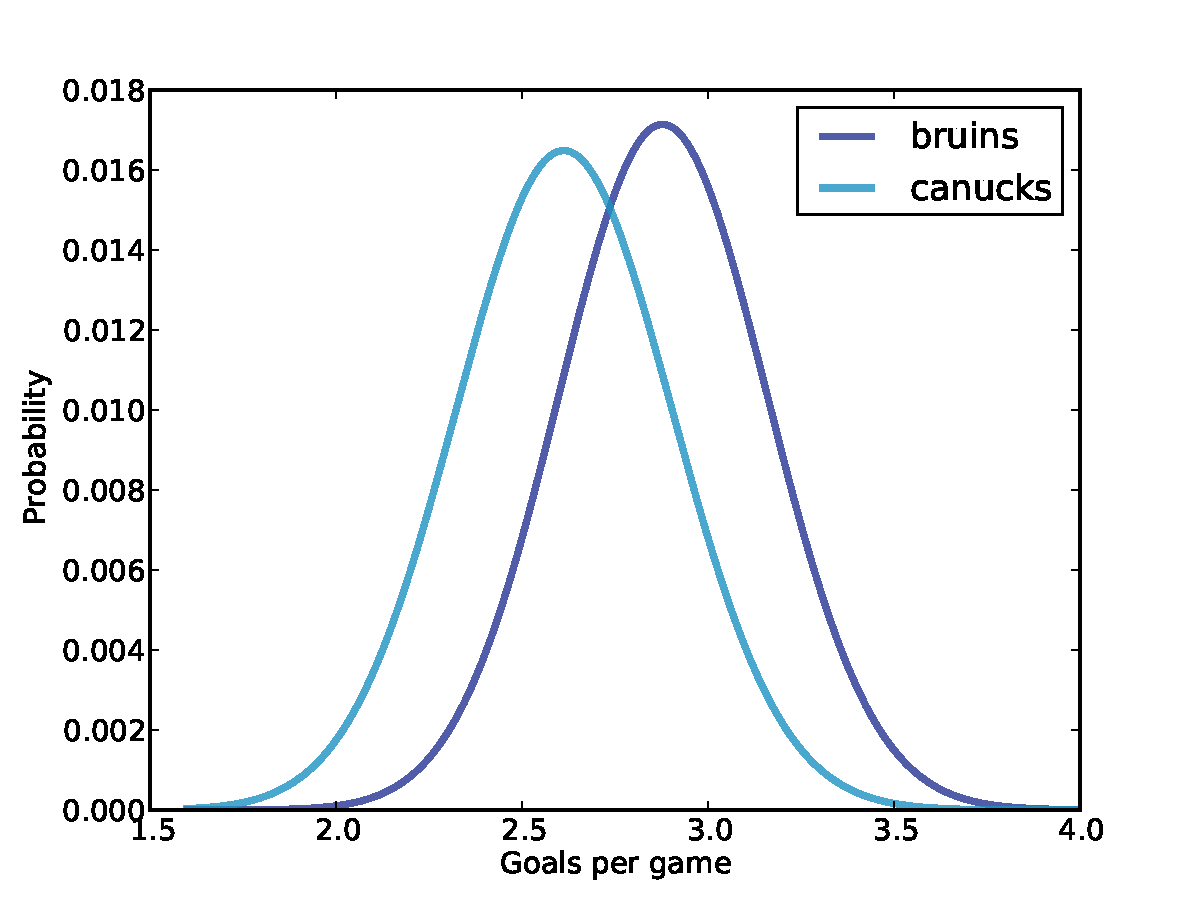
\includegraphics[height=2.5in]{figs/hockey1.pdf}}
\caption{Posterior distribution of the number of
goals per game.}
\label{fig.hockey1}
\end{figure}

Now we can compute the likelihood of seeing a team with a hypothetical
value of {\tt lam} score {\tt k} goals in a game:

\begin{verbatim}
# class Hockey

    def Likelihood(self, hypo, data):
        lam = hypo
        k = data
        like = thinkbayes.EvalPoissonPmf(lam, k)
        return like
\end{verbatim}

Each hypothesis is a possible value of $\lambda$;  {\tt
  data} is the observed number of goals, {\tt k}.

With the likelihood function in place, we can make a suite for each
team and update them with the scores from the first four games.

\begin{verbatim}
    suite1 = Hockey('bruins')
    suite1.UpdateSet([0, 2, 8, 4])
     
    suite2 = Hockey('canucks')
    suite2.UpdateSet([1, 3, 1, 0])
\end{verbatim}  

Figure~\ref{fig.hockey1} shows the resulting posterior distributions
for {\tt lam}.  Based on the first four games, the most likely
values for {\tt lam} are 2.6 for the Canucks and 2.9 for the Bruins.


\section{The Meta-Pmf}
\label{meta-pmf}

\begin{figure}
% hockey.py
\centerline{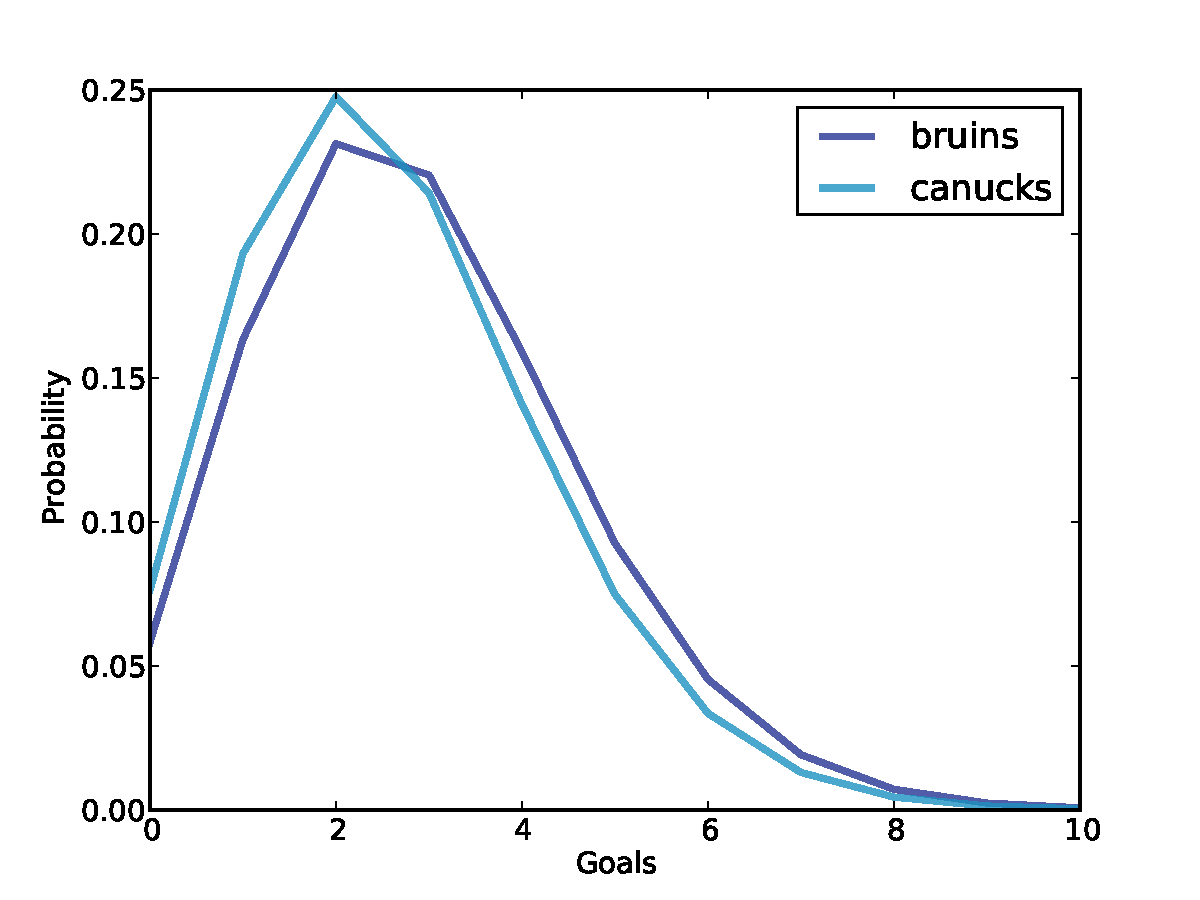
\includegraphics[height=2.5in]{figs/hockey2.pdf}}
\caption{Distribution of goals in a single game.}
\label{fig.hockey2}
\end{figure}

To compute the probability that each team wins the next game,
we need to compute the distribution of goals for each team.

If we knew the value of {\tt lam} exactly, we could use the
Poisson distribution again.  \verb"thinkbayes" provides a
method that computes a truncated approximation of a Poisson
distribution:

\begin{verbatim}
def MakePoissonPmf(lam, high):
    pmf = Pmf()
    for k in xrange(0, high+1):
        p = EvalPoissonPmf(lam, k)
        pmf.Set(k, p)
    pmf.Normalize()
    return pmf
\end{verbatim}  

The range of values in the computed Pmf is from 0 to {\tt high}.
So if the value of {\tt lam} were exactly 3.4, we would compute:

\begin{verbatim}
lam = 3.4
goal_dist = thinkbayes.MakePoissonPmf(lam, 10)
\end{verbatim}

I chose the upper bound, 10, because the probability of scoring
more than 10 goals in a game is quite low.

That's simple enough so far; the problem is that we don't know
the value of {\tt lam} exactly.  Instead, we have a distribution
of possible values for {\tt lam}.

For each value of {\tt lam}, the distribution of goals is Poisson.
So the overall distribution of goals is a mixture of these
Poisson distributions, weighted according to the probabilities
in the distribution of {\tt lam}.

\verb"thinkbayes" provides a method that computes mixtures
of distributions:

\begin{verbatim}
def MakeMixture(metapmf):
    mix = Pmf()
    for pmf, p1 in metapmf.Items():
        for x, p2 in pmf.Items():
            mix.Incr(x, p1 * p2)
    return mix
\end{verbatim}  

{\tt metapmf} is a Meta-Pmf, which means that it is a Pmf that
contains Pmfs.  If you find the Meta-Pmf confusing; it might
help to think about how you would generate a random value from
a Meta-Pmf.  First you would choose a Pmf according to the
probabilities in the Meta-Pmf.  Then you would choose a value
according to the probabilities in the chosen Pmf.

\verb"MakeMixture" computes the distribution of the resulting
values.

Given the posterior distribution of {\tt lam}, here's the code
that makes the distribution of goals:

\begin{verbatim}
def MakeGoalPmf(suite):
    metapmf = thinkbayes.Pmf()
    high = 10

    for lam, prob in suite.Items():
        pmf = thinkbayes.MakePoissonPmf(lam, high)
        metapmf.Set(pmf, prob)

    mix = thinkbayes.MakeMixture(metapmf)
    return mix
\end{verbatim}  

For each value of {\tt lam} we make a Poisson Pmf and add it to the
Meta-Pmf.  Then we use \verb"MakeMixture" to compute the mixture.  If
the Meta-Pmf makes your head hurt, don't panic.  We are past the hard
part of the problem now; everything else is easy.

Figure~\ref{fig.hockey2} shows the resulting distribution of goals for
the Bruins and Canucks.  As expected, the Bruins are less likely to
score 3 goals or fewer in the next game, and more likely to score 4 or
more.


\section{The probability of winning}

\begin{figure}
% hockey.py
\centerline{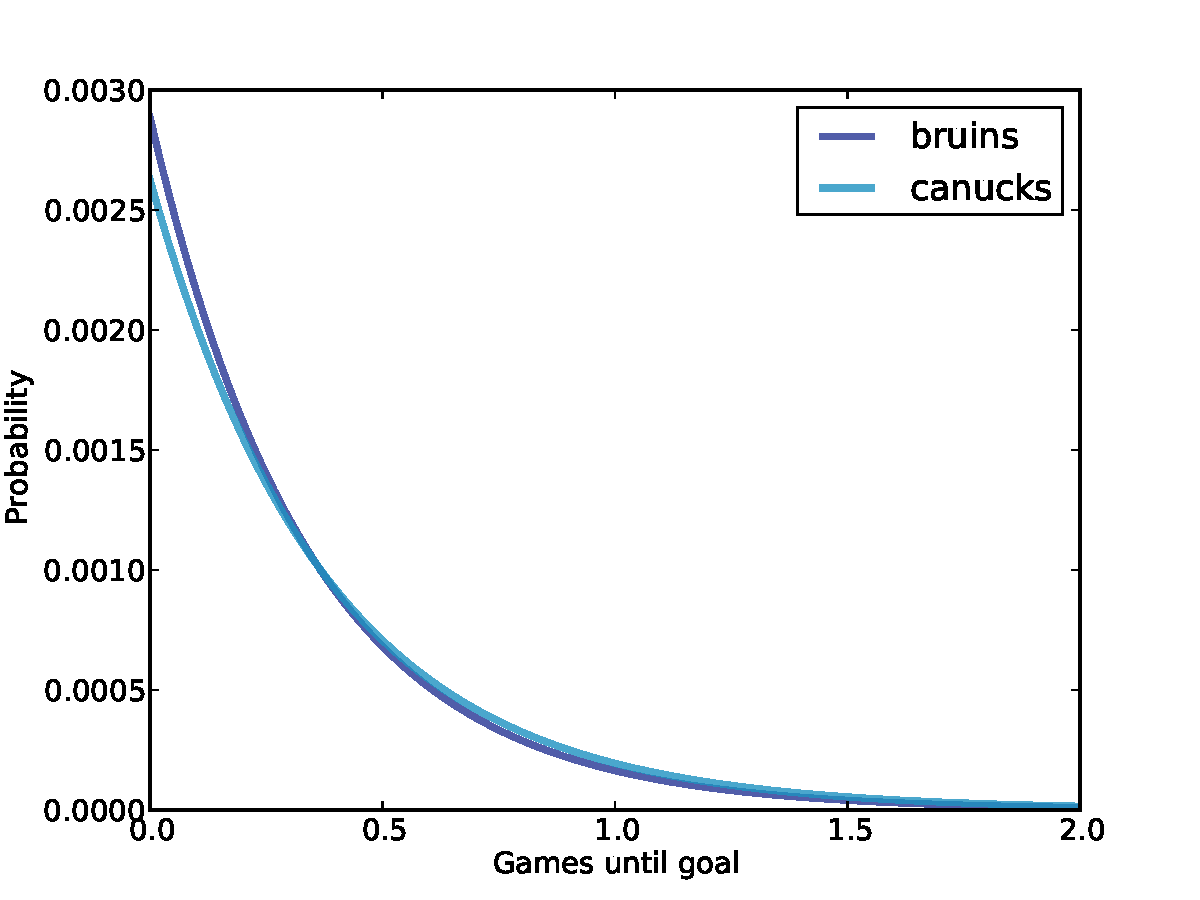
\includegraphics[height=2.5in]{figs/hockey3.pdf}}
\caption{Distribution of time between goals.}
\label{fig.hockey3}
\end{figure}

To get the probability of winning, first we compute the
distribution of the goal differential:

\begin{verbatim}
    goal_dist1 = MakeGoalPmf(suite1)
    goal_dist2 = MakeGoalPmf(suite2)
    diff = goal_dist1 - goal_dist2
\end{verbatim}  

The subtraction operator invokes the \verb"__sub__" method
in {\tt Pmf}, which enumerates pairs of values and computes
the difference.

If the goal differential is positive, the Bruins win; if negative, the
Canucks win; if 0, it's a tie:

\begin{verbatim}
    p_win = diff.ProbGreater(0)
    p_loss = diff.ProbLess(0)
    p_tie = diff.Prob(0)
\end{verbatim}  

With the distributions from the previous section, \verb"p_win"
is 46\%, \verb"p_loss" is 37\%, and \verb"p_tie" is 17\%.

In the event of a tie at the end of regulation play, the teams play
overtime periods until one team scores.  Since the game ends
immediately when the first goal is scored, this overtime format
is known as ``sudden death.''


\section{Sudden death}

To compute the probability of winning in a sudden death overtime,
the important statistic is not goals per game, but time until the
first goal.  The assumption that goal-scoring is a Poisson process
is helpful here, because it implies that the time between goals
is exponentially distributed.

Given {\tt lam}, we can compute the time between goals like this: 

\begin{verbatim}
lam = 3.4
time_dist = thinkbayes.MakeExponentialPmf(lam, high=2, n=101)
\end{verbatim}  

{\tt high} is the upper bound of the distribution.  In this case
I chose 2, because the probability of going more than two games
without scoring is small.  {\tt n} is the number of values in
the Pmf.

If we know {\tt lam} exactly, that's all there is to it.
But we don't; instead we have a posterior
distribution of possible values.  So as we did with the distribution
of goals, we have to make a Meta-Pmf and compute a mixture of
Pmfs.

\begin{verbatim}
def MakeGoalTimePmf(suite):
    metapmf = thinkbayes.Pmf()

    for lam, prob in suite.Items():
        pmf = thinkbayes.MakeExponentialPmf(lam, high=2, n=2001)
        metapmf.Set(pmf, prob)

    mix = thinkbayes.MakeMixture(metapmf)
    return mix
\end{verbatim}  

Figure~\ref{fig.hockey2} shows the resulting distributions.  For
time values less than one period (one third of a game), the Bruins
are more likely to score.  The time until the Canucks score is
more likely to be longer.

I set the number of values, {\tt n},
fairly high in order to minimize the number of ties, since it is not
actually possible for both teams to score simultaneously.

Now we can compute the probability that the Bruins score first:

\begin{verbatim}
    time_dist1 = MakeGoalTimePmf(suite1)
    time_dist2 = MakeGoalTimePmf(suite2)
    p_overtime = thinkbayes.PmfProbLess(time_dist1, time_dist2)
\end{verbatim}  

For the Bruins, the probability of winning in overtime is 52\%.
Finally, we can compute the total probability of winning:

\begin{verbatim}
    p_tie = diff.Prob(0)
    p_overtime = thinkbayes.PmfProbLess(time_dist1, time_dist2)

    p_win = diff.ProbGreater(0) + p_overtime * p_tie
\end{verbatim}  

So the overall chance of winning the next game is 55\%.
To win the series, the Bruins can either win the next two games
or split the next two and win the third.  Again, we can compute
the total probability:

\begin{verbatim}
    # win the next two
    p_series = p_win**2

    # split the next two, win the third
    p_series += 2 * p_win * (1-p_win) * p_win
\end{verbatim}  

The Bruins chance of winning the series is 57\%.  And in 2011,
they did.


\section{Opportunities for improvement}

Solving problems like this is almost always iterative.  In general,
you want to start with something simple that yields an approximate
answer, then look for opportunities to improve.

In this example, I would consider these options:

\begin{itemize}

\item I chose a prior based on the average goals per game for each
  team.  But this statistic is averaged across all opponents.  Against
  a particular opponent, we might expect more variability.  For
  example, if the team with the best offense plays the team with the
  worst defense, the expected goals per game might be several standard
  deviations above the mean.

\item For data I used only the first four games of the championship
  series.  Assuming that the same teams played each other during the
  regular season, I could use the results from those games as well.
  One complication is that the composition of teams changes during
  the season due to trades and injuries.  So it might be best to
  give more weight to recent games.

\item To take advantage of all available information, we could
  use results from all regular season games to estimate each team's
  goal scoring rate, possibly adjusted by estimating
  an additional factor for each pairwise match-up.  This approach
  would be more complicated, but it is still feasible.
  [[Forward reference to chess example]]

\end{itemize}

For the first option, we could use the results from the regular season
to estimate the variability across all pairwise match-ups.  Thanks to
Dirk Hoag at \url{http://forechecker.blogspot.com/}, I was able to get
the number of goals scored during regulation play (not overtime) for
each game in the regular season.

Teams in different conferences only play each other one or two
times in the regular season, so I focused on pairs that played
each other 4--6 times.  For each pair, I computed the average
goals per game, which is an estimate of $\lambda$, then plotted
the distribution of these estimates.

The mean of these estimates is 2.8, again, but the standard
deviation is 0.85, substantially higher than what we got computing
one estimate for each team.

If we run the analysis again with the higher-variance prior, the
probability that the Bruins win the series is 80\%, substantially
higher than the result with the low-variance prior, 57\%.

So this is another example where the results are sensitive to the
prior.  In general, if the variability in the prior is too high, the
extreme values will be contradicted by data.  But if the
variability is too low, the effective range of the prior is too
narrow, and the data may not be able to correct the error.  So it is
usually a good idea to err on the side of a more generous prior.

The code and data for this chapter are available from
\url{http://thinkbayes.com/hockey.py} and
\url{http://thinkbayes.com/hockey_data.csv}.


\section{Exercises}

\begin{exercise}

If buses arrive at a bus stop every 20 minutes, and you
arrive at the bus stop at a random time, your wait time until
the bus arrives is uniformly distributed from 0 to 20 minutes.

But in reality, there is variability in the time between
buses.  Suppose you are waiting for a bus, and you know the historical
distribution of time between buses.  Compute your distribution
of wait times.

Hint: Suppose that the time between buses is either
10 or 20 minutes with equal probability.  What is the probability
that you arrive during one of the 20 minute intervals?

\end{exercise}


\begin{exercise}

Suppose that passengers arriving at the bus stop are well-modeled
by a Poisson process with parameter $\mu$.  If you arrive at the
stop and find 3 people waiting, what is your posterior distribution
for the time since the last bus arrived.

\end{exercise}


\begin{exercise}

Suppose that you are an ecologist sampling the insect population in
a new environment.  You deploy 100 traps in a test area and come back
the next day to check on them.  You find that 37 traps have been
triggered, trapping an insect inside.  Once a trap triggers, it
cannot trap another insect until it has been reset.

If you reset the traps and come back in two days, how many traps
do you expect to find triggered?  Compute a posterior predictive
distribution for the number of traps.

\end{exercise}


\begin{exercise}

Suppose you are the manager of an apartment building with
100 light bulbs in common areas.  It is your responsibility
to replace light bulbs when they break.

On January 1, all 100 bulbs are working.  When you inspect
them on February 1, you find 3 light bulbs out.  If you
come back on April 1, how many light bulbs do you expect to
find broken?

In the previous exercise, you could reasonably assume that an event is
equally likely at any time.  For light bulbs, the likelihood of
failure depends on the age of the bulb.  Specifically, old bulbs
have an increasing failure rate due to evaporation of the filament.

This problem is more open-ended than some; you will have to make
modeling decisions.  You might want to read about the Weibull
distribution
(\url{http://en.wikipedia.org/wiki/Weibull_distribution}).
Or you might want to look around for information about
light bulb survival curves.

\end{exercise}


\chapter{Two dimensions}
\label{paintball}

\section{Paintball}

\begin{figure}
% paintball.py
\centerline{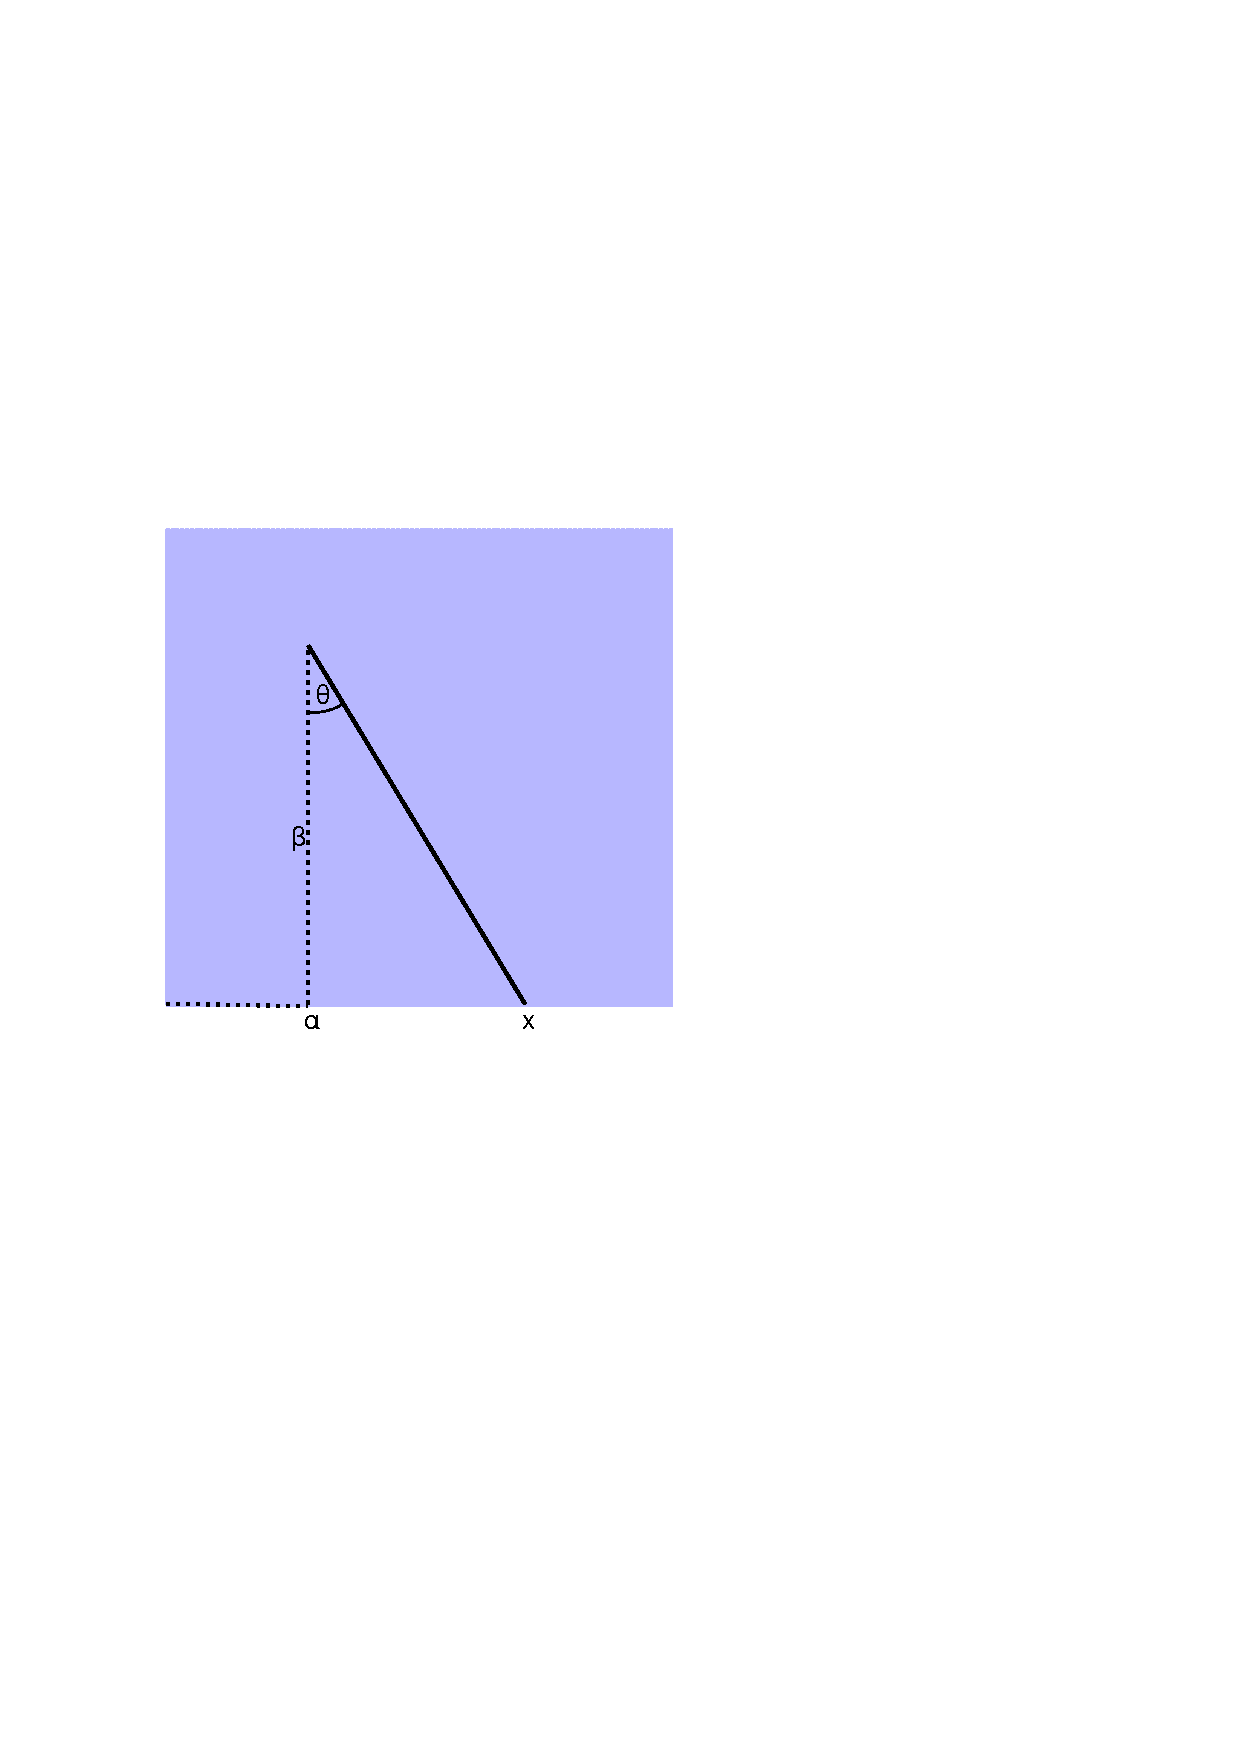
\includegraphics[height=2.5in]{figs/paintball.pdf}}
\caption{Diagram of the layout for the paintball problem.}
\label{fig.paintball}
\end{figure}

Paintball is a sport in which competing teams try to shoot each other
with guns that fire paint-filled pellets that break on impact, leaving
a colorful mark on the target.  It is usually played in a demarcated
area decorated with barriers and other objects that can be
used as cover.

Suppose you are playing paintball in an indoor arena 30 feet
wide and 50 feet long.  You are standing near one of the 30 foot
walls, and you suspect that one of your opponents has taken cover
nearby.  Along the wall, you see several paint spatters, all the same
color, that you think your opponent fired recently.

The spatters are at 15, 16, 18 and 21 feet, measured from the
lower-left corner of the room.  Based on these data, where do you
think your opponent is hiding?

Figure~\ref{fig.paintball} shows a diagram of the arena.  Using the
lower-left corner of the room as the origin, I denote the unknown
location of the shooter with coordinates $\alpha$ and $\beta$, or {\tt
  alpha} and {\tt beta}.  The location of a paint spatter is labeled
{\tt x}.  The angle the opponent shoots at is $\theta$ or {\tt theta}.

The paintball problem in this chapter is a slightly modified version
of the lighthouse problem, a common example of Bayesian analysis.  My
notation follows the presentation of the problem in Sivia, {\it Data
  Analysis: a Bayesian Tutorial, Second Edition}.


\section{Trigonometry}

\begin{figure}
% paintball.py
\centerline{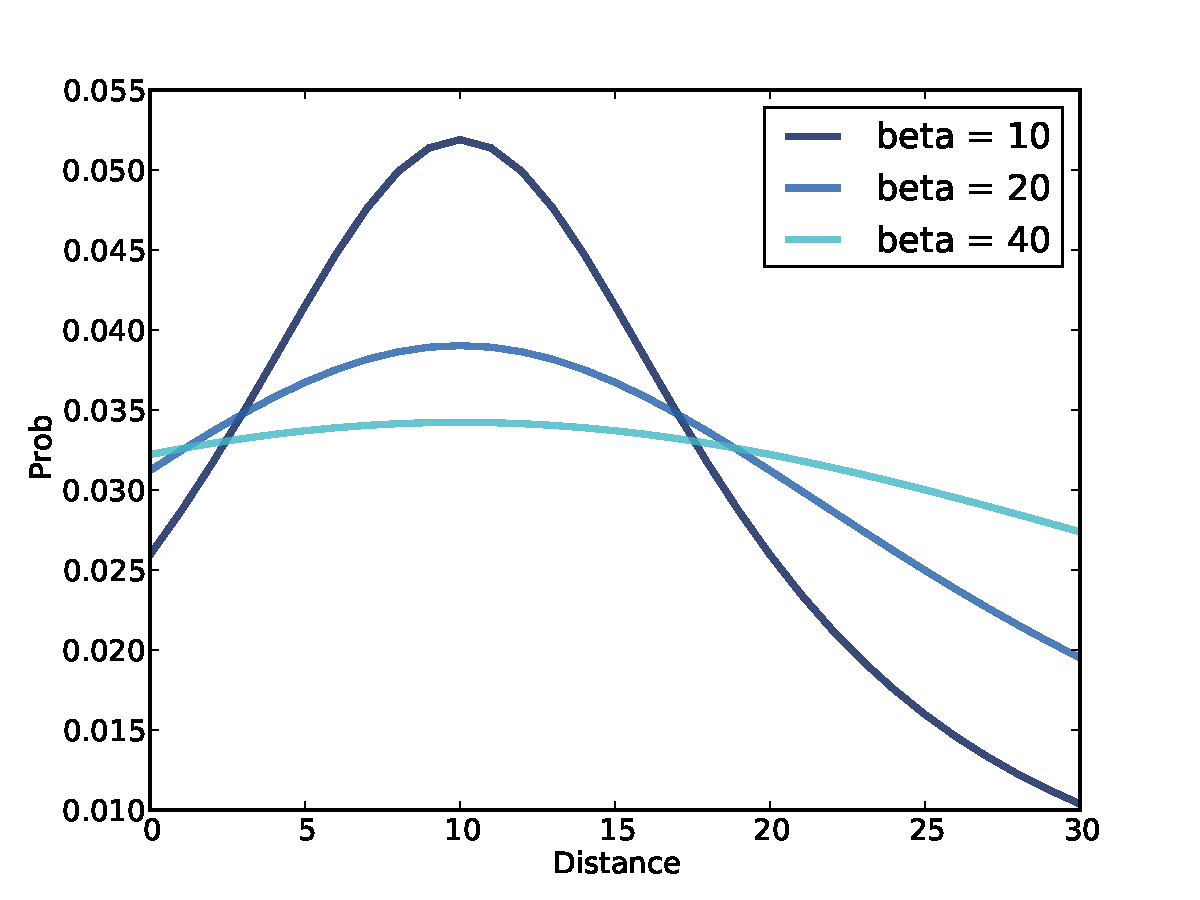
\includegraphics[height=2.5in]{figs/paintball1.pdf}}
\caption{PMF of location given {\tt alpha} for several values of {\tt beta}.}
\label{fig.paintball1}
\end{figure}

At least initially, let's assume that the opponent is equally likely
to shoot at any angle.  If that's the case, he is most likely to hit
the wall at location {\tt alpha}, and less likely to hit the wall far
away from {\tt alpha}.

With a little trigonometry, we can compute the probability of hitting
any spot along the wall.  Imagine that the shooter fires a shot at
angle $\theta$ then turns slightly and fires again at angle $\theta +
\Delta\theta$.

The first pellet would hit the wall at location $x$, where
%
\[ x - \alpha = \beta \tan \theta \]
%
The second pellet would hit the wall at location $x'$, where
%
\[ x' = x + \frac{dx}{d\theta} \Delta\theta \]
%
The derivative $dx/d\theta$ is what I'll call the ``strafing speed'',
which is the speed of the target location along the wall as $\theta$
increases.  The probability of hitting a given point on the wall is
inversely related to strafing speed.

Taking the derivative of the first equation yields
%
\[ \frac{dx}{d\theta} = \beta / \cos^2 \theta \]
%
And solving the same equation for $\theta$ yields
%
\[ \theta = tan^{-1} \left[ \frac{x - \alpha}{\beta} \right] \]
%
So if we know the coordinates of the shooter and a location 
along the wall, we can compute strafing speed:

\begin{verbatim}
def StrafingSpeed(alpha, beta, x):
    theta = math.atan2(x - alpha, beta)
    speed = beta / math.cos(theta)**2
    return speed
\end{verbatim}

{\tt alpha} and {\tt beta} are the coordinates of the shooter;
{\tt x} is the location of a paint spatter.  The result is
the derivative of {\tt x} with respect to {\tt theta}.

Now we can compute the probability of hitting any spot along
the wall.  {\tt MakeLocationPmf} takes the coordinates of
the shooter, {\tt alpha} and {\tt beta}, and a list of possible
values of {\tt x}, {\tt locations}.

\begin{verbatim}
def MakeLocationPmf(alpha, beta, locations):
    pmf = thinkbayes.Pmf()
    for x in locations:
        prob = 1.0 / StrafingSpeed(alpha, beta, x)
        pmf.Set(x, prob)
    pmf.Normalize()
    return pmf
\end{verbatim}

For each location, the probability is inversely related to
strafing speed.  The result is a Pmf of locations and their
probabilities.

Figure~\ref{fig.paintball1} shows the Pmf of location with
{\tt alpha = 10} and a range of values for {\tt beta}.  As
expected, the most likely impact location is {\tt x = 10},
and as {\tt beta} increases, so does the spread of the Pmf.


\section{The suite}

\begin{figure}
% paintball.py
\centerline{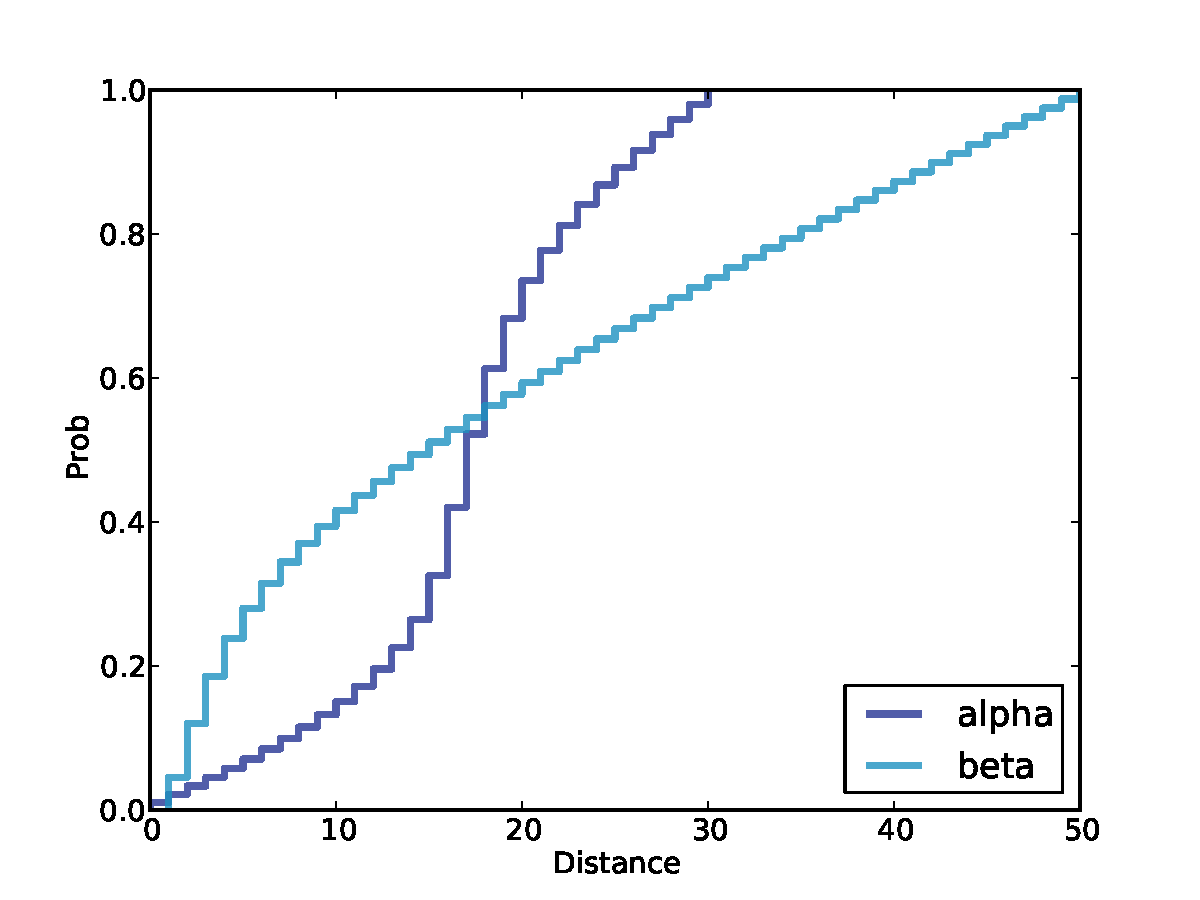
\includegraphics[height=2.5in]{figs/paintball2.pdf}}
\caption{Posterior CDFs for {\tt alpha} and {\tt beta}, given the data.}
\label{fig.paintball2}
\end{figure}

Next we define a suite of hypotheses for the coordinates of the
shooter.  Each value in the suite is a pair of coordinates: {\tt
  (alpha, beta)}.

Here is the function that initializes the suite:

\begin{verbatim}
class Paintball(thinkbayes.Suite, thinkbayes.Joint):

    def __init__(self, alphas, betas, locations):
        self.locations = locations
        pairs = [(alpha, beta) 
                 for alpha in alphas 
                 for beta in betas]
        thinkbayes.Suite.__init__(self, pairs)
\end{verbatim}

{\tt Paintball} inherits from {\tt Suite}, which we have seen before,
and {\tt Joint}, which I will explain soon.

{\tt alphas} is the list of possible values for {\tt alpha}; {\tt
  betas} is the list of values for {\tt beta}.  {\tt pairs} is a list
of all {\tt (alpha, beta)} pairs.

{\tt locations} is a list of possible impact locations along
the wall; it is stored for use in {\tt Likelihood}.

The room is 30 feet wide and 50 feet long, so here's the code that
creates the suite:

\begin{verbatim}
    alphas = range(0, 31)
    betas = range(1, 51)
    locations = range(0, 31)

    suite = Paintball(alphas, betas, locations)
\end{verbatim}

This prior distribution assumes that all locations in the room are
equally likely.  Given a map of the room, we might choose a more
detailed prior, but we'll start simple.


\section{Likelihood}

All we need now is a likelihood function:

\begin{verbatim}
    def Likelihood(self, hypo, data):
        alpha, beta = hypo
        x = data
        pmf = MakeLocationPmf(alpha, beta, self.locations)
        like = pmf.Prob(x)
        return like
\end{verbatim}

{\tt hypo} contains the hypothetical coordinates of the shooter.
{\tt data} contains an impact location along the wall.

{\tt pmf} contains the probability of each location, given the
coordinates of the shooter.  From this Pmf, we select the probability
of the particular location that was observed.

And we're done.  To update the suite, we can use {\tt UpdateSet},
which is inherited from {\tt Suite}.

\begin{verbatim}
suite.UpdateSet([15, 16, 18, 21])
\end{verbatim}

The result is a distribution that maps each {\tt (alpha, beta)} pair
to a posterior probability.  Since each value in the posterior
distribution is a pair of variables, this distribution is called a
``joint distribution'' of the two variables.


\section{Joint distributions}

Given the joint distribution, we can compute the distributions
of each variable independently, which are called the ``marginal
distributions.''

{\tt thinkbayes.Joint} provides a method that computes marginal
distributions:

\begin{verbatim}
# class Joint:

    def Marginal(self, i):
        pmf = Pmf()
        for vs, prob in self.Items():
            pmf.Incr(vs[i], prob)
        return pmf
\end{verbatim}

{\tt i} is the index of the variable we want; in this example
{\tt i=0} indicates the distribution of {\tt alpha}, and
{\tt i=1} indicates the distribution of {\tt beta}.

Here's the code that extracts the marginal distributions:

\begin{verbatim}
    marginal_alpha = suite.Marginal(0)
    marginal_beta = suite.Marginal(1)
\end{verbatim}

Figure~\ref{fig.paintball2} shows the results (converted to CDFs).
The median value for {\tt alpha} is 18, near the center of mass of
the observed spatters.  For {\tt beta}, the most likely values are
close to the wall, but beyond 10 feet the distribution is almost
uniform, which indicates that the data do not distinguish strongly
between these possible locations.

Given the posterior marginals, we can compute credible intervals
for each coordinate independently:

\begin{verbatim}
    print 'alpha CI', marginal_alpha.CredibleInterval(50)
    print 'beta CI', marginal_beta.CredibleInterval(50)
\end{verbatim}

The 50\% credible intervals are {\tt (14, 21)} for {\tt alpha} and
{\tt (5, 31)} for {\tt beta}.  So the data provide evidence that the
shooter is in the near side of the room.  But it is not strong
evidence.  The 90\% credible interval covers most of the room!


\section{Conditional distributions}

\begin{figure}
% paintball.py
\centerline{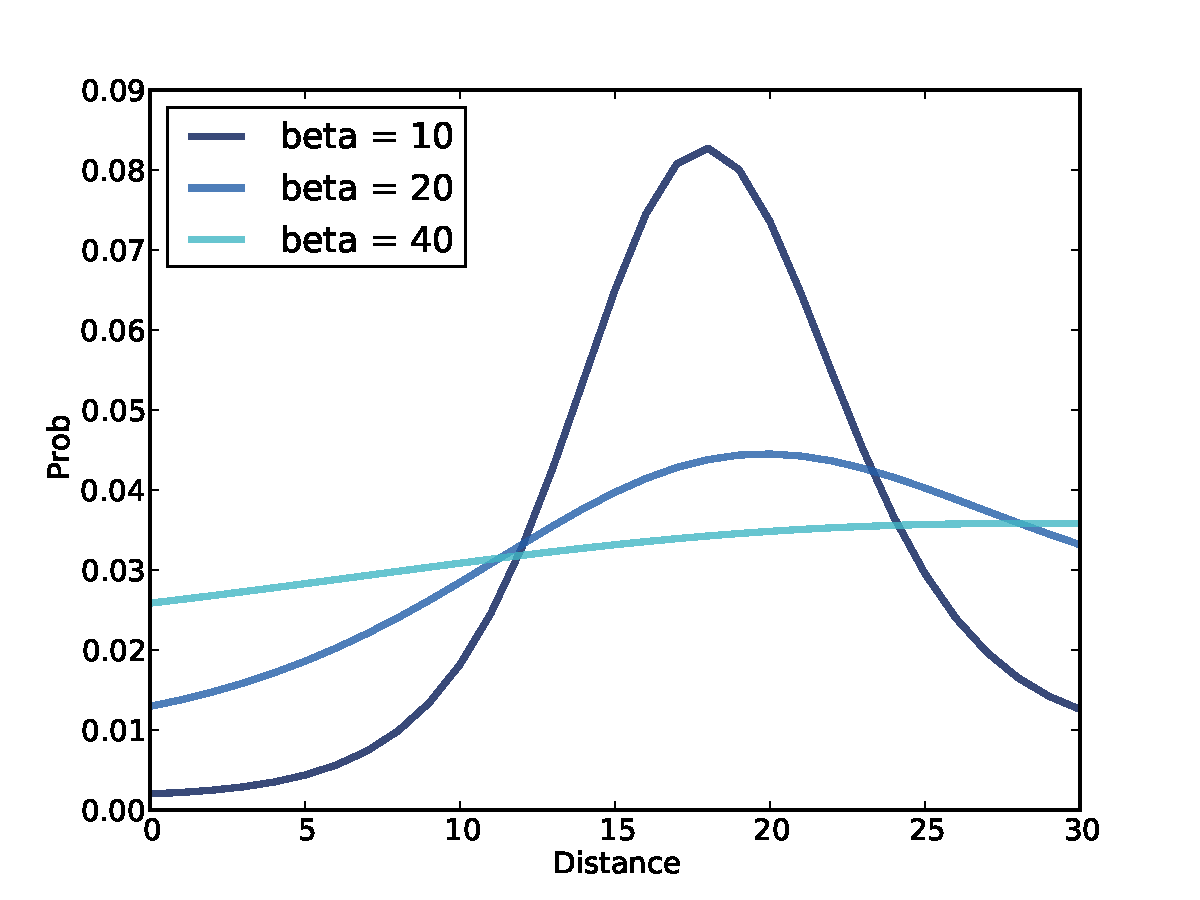
\includegraphics[height=2.5in]{figs/paintball3.pdf}}
\caption{Distributions for {\tt alpha} conditioned on several values
of {\tt beta}.}
\label{fig.paintball3}
\end{figure}

The marginal distributions contain information about the variables
independently, but they do not capture the dependence between
variables, if any.

One way to visualize dependence is by computing conditional
distributions.  {\tt thinkbayes.Joint} provides a method that
does just that:

\begin{verbatim}
    def Conditional(self, i, j, val):
        pmf = Pmf()
        for vs, prob in self.Items():
            if vs[j] != val: continue
            pmf.Incr(vs[i], prob)

        pmf.Normalize()
        return pmf
\end{verbatim}

Again, {\tt i} is the index of the variable we want; {\tt j}
is the index of the conditioning variable, and {\tt val} is the
conditional value.

The result is the distribution of the $i$th variable under the
condition that the $j$th variable is {\tt val}.

For example, the following code computes the conditional distributions
of {\tt alpha} for a range of values of {\tt beta}:

\begin{verbatim}
    betas = [10, 20, 40]

    for beta in betas:
        cond = suite.Conditional(0, 1, beta)
        myplot.Pmf(cond)
\end{verbatim}

Figure~\ref{fig.paintball3} shows the results, which we could
fully describe as ``posterior conditional marginal distributions!''

The shapes of these distributions are different, which indicates
that the variables are not independent.  If we know somehow that
{\tt beta = 10}, then we can be fairly confident about {\tt alpha}.
But as {\tt beta} increases, so does the spread in {\tt alpha}.


\section{Credible intervals}

\begin{figure}
% paintball.py
\centerline{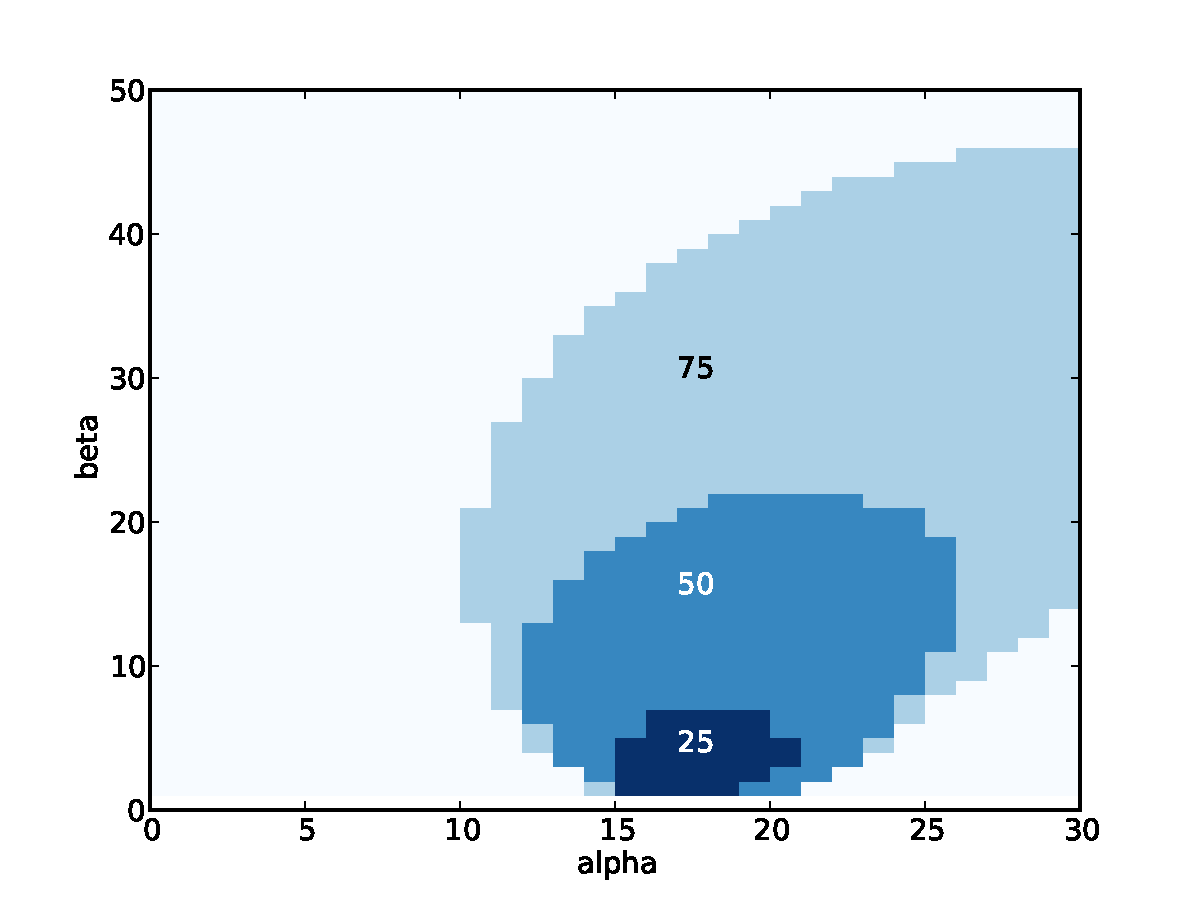
\includegraphics[height=2.5in]{figs/paintball5.pdf}}
\caption{Credible intervals for the coordinates of the opponent.}
\label{fig.paintball5}
\end{figure}

Another way to visualize the posterior joint distribution is to
compute credible intervals.  Last time we looked at credible intervals,
I skipped over an important point: for a given distribution, there
are many intervals with the same level of credibility.  For example,
if you want a 50\% credible interval, you could choose any set of
values whose probability adds up to 50\%.

When the values are one-dimensional, it is most common to choose
the ``central credible interval;'' for example, the central 50\%
credible interval contains all values between the 25th and 75th
percentiles.

In multiple dimensions it is less obvious what the right credible
interval should be.  The best choice might depend on context.  But
one common choice is the maximum likelihood credible interval, which
contains the most likely values that add up to 50\% (or some other
percentage).

{\tt thinkbayes.Joint} provides a method that computes maximum
likelihood credible intervals. 

\begin{verbatim}
# class Joint:

    def MaxLikeInterval(self, percentage=90):
        interval = []
        total = 0

        t = [(prob, val) for val, prob in self.Items()]
        t.sort(reverse=True)

        for prob, val in t:
            interval.append(val)
            total += prob
            if total >= percentage/100.0:
                break

        return interval
\end{verbatim}

The first step is to make a list of the values in the suite,
sorted in descending order by probability.  Next we traverse the
list, adding each value to the interval, until the total
probability exceeds {\tt percentage}.  The result is a list
of values from the suite.

To visualize these intervals, I wrote a function that ``colors''
each value according to how many intervals it appears in:

\begin{verbatim}
def MakeCrediblePlot(suite):
    d = dict((pair, 0) for pair in suite.Values())

    percentages = [75, 50, 25]
    for p in percentages:
        interval = suite.MaxLikeInterval(p)
        for pair in interval:
            d[pair] += 1

    myplot.Contour(d, contour=False, pcolor=True)
    myplot.Show()
\end{verbatim}

{\tt d} is a dictionary that maps from each value in the suite
to the number of intervals it appears in.  The loop computes intervals
for several percentages and modifies {\tt d}.  Then I use functions
from {\tt myplot} to generate a pseudocolor plot.

Figure~\ref{fig.paintball5} shows the result.  The 25\% credible
interval is the darkest region near the bottom wall.  For higher
percentages, the credible interval is bigger, of course, and skewed
toward the right side of the room.





\chapter{Approximate Bayesian Computation}

\section{The Variability Hypothesis}

I have a soft spot for crank science.  Recently I visited Norumbega
Tower, which is an enduring monument to the crackpot theories of Eben
Norton Horsford, inventor of double-acting baking powder and fake
history.  But that's not what this chapter is about.

This article is about the Variability Hypothesis, which

\begin{quote}
"originated in the early nineteenth century with Johann Meckel, who
  argued that males have a greater range of ability than females,
  especially in intelligence. In other words, he believed that most
  geniuses and most mentally retarded people are men. Because he
  considered males to be the 'superior animal,' Meckel concluded that
  females' lack of variation was a sign of inferiority."

From \url{http://en.wikipedia.org/wiki/Variability_hypothesis}.
\end{quote}

I particularly like that last part, because I suspect that if it turns
out that women are actually more variable, Meckel would take that as a
sign of inferiority, too.  Anyway, you will not be surprised to hear
that evidence for the Variability Hypothesis is not strong.

Nevertheless, it came up in my class recently when we looked at data
from the CDC's Behavioral Risk Factor Surveillance System (BRFSS),
specifically the self-reported heights of adult American men and women.
The dataset includes responses from 154407 men and 254722 women.
Here's what we found:

\begin{itemize}

\item The average height for men is 178 cm; the average height for
  women is 163 cm.  So men are taller, on average.  No surprises so
  far.

\item For men the standard deviation is 7.7 cm; for women is it 7.3
  cm.  So in absolute terms, men's heights are more variable.

\item But to compare variability between groups, it is more meaningful
  to use the coefficient of variation (CV), which is the standard
  deviation divided by the mean.  It is a dimensionless measure of
  variability relative to scale.  For men CV is 0.0433; for women it
  is 0.0444.

\end{itemize}

That's very close, so we could conclude that this dataset provides
little support for the Variability Hypothesis.  But we can use
Bayesian methods to make that conclusion more precise.  And answering
this question gives me a chance to demonstrate some techniques
for working with large datasets.

I will proceed in a few steps:

\begin{enumerate}

\item We'll start with the simplest implementation, but it only works
  for datasets smaller than 1000 values.

\item By computing probabilities under a log transform, we can scale
  up to the full size of the dataset, but the computation gets slow.

\item Finally, we speed things up substantially with Approximate
  Bayesian Computation, also known as ABC.

\end{enumerate}

You can download the code in this chapter from
\url{http://thinkbayes.com/variability.py}.


\section{Mean and standard deviation}

In Chapter~\ref{paintball} we estimated two parameters simultaneously
using a joint distribution.  In this chapter we use the same
method to estimate the parameters of a normal distribution:
the mean, {\tt mu}, and the standard deviation, {\tt sigma}.

For this problem, I defined a Suite called {\tt Height} that
represents a map from each {\tt mu, sigma} pair to its probability:

\begin{verbatim}
class Height(thinkbayes.Suite, thinkbayes.Joint):

    def __init__(self, mus, sigmas):
        thinkbayes.Suite.__init__(self)

        self.mus = mus
        self.sigmas = sigmas

        pairs = [(mu, sigma) 
                 for mu in mus
                 for sigma in sigmas]

        thinkbayes.Suite.__init__(self, pairs)
\end{verbatim}

{\tt mus} is a sequence of possible values for {\tt mu}; {\tt sigmas}
is a sequence of values for {\tt sigma}.  The prior distribution
is uniform over all {\tt mu, sigma} pairs.

The likelihood function is easy.  Given hypothetical values
of {\tt mu} and {\tt sigma}, we compute the likelihood
of a particular value, {\tt x}.  That's what {\tt EvalGaussianPdf}
does, so all we have to do is use it:

\begin{verbatim}
# class Height

    def Likelihood(self, hypo, data):
        x = data
        mu, sigma = hypo

        like = thinkbayes.EvalGaussianPdf(mu, sigma, x)
        return like
\end{verbatim}

If you have studied statistics from a mathematical perspective,
you know that when you evaluate a PDF, you get a probability
density.  In order to get a probability, you have to integrate
probability densities over some range.

But for our purposes, we don't need a probability; we just
need something proportional to the probability we want.
A probability density does that job nicely.

The hardest part of this problem turns
out to be choosing appropriate ranges for {\tt mus} and
{\tt sigmas}.  If the range is too small, we omit some
possibilities with non-negligible probability and get the
wrong answer.  If the range is too big, we get the right answer,
but waste computational power.

So this is an opportunity to use classical estimation techniques to
make Bayesian techniques more efficient.  Specifically, we can use
classical estimators to find a likely location for {\tt mu} and {\tt
  sigma}, and use the standard errors of those estimates to choose a
likely spread.

If the true parameters of the distribution are $\mu$ and
$\sigma$, and we take a sample of $n$ values, an estimator
of $\mu$ is
%
\[ \bar{x} = \frac{1}{n} \sum_i x_i \]
%
and an estimator of $\sigma^2$ is
%
\[ S^2 = \frac{1}{n-1} \sum_i (x_i - \bar{x})^2 \]
%
The standard error of the estimated $\mu$ is
%
\[ S / \sqrt{n} \]
%
and the standard error of the estimated $\sigma$ is
%
\[ S / \sqrt{2 (n-1)}\]
%
Here's the code to compute all that:

\begin{verbatim}
def FindPriorRanges(xs, num_points, num_stderrs=3.0):

    # compute xbar and S
    n = len(xs)
    xbar, S2 = thinkstats.MeanVar(xs)
    S = math.sqrt(S2)

    # compute ranges for xbar and S
    stderr_xbar = S / math.sqrt(n)
    mus = MakeRange(xbar, stderr_xbar)

    stderr_S = S / math.sqrt(2 * (n-1))
    sigmas = MakeRange(S, stderr_S)

    return mus, sigmas
\end{verbatim}

{\tt xs} is the dataset.  \verb"num_points" is the desired number of
values in the range.  \verb"num_stderrs" is the width of the range on
each side of the estimate, in number of standard errors.  The return
value is a pair of sequences, {\tt mus} and {\tt sigmas}.

Here's {\tt MakeRange}:

\begin{verbatim}
    def MakeRange(estimate, stderr):
        spread = stderr * num_stderrs
        array = numpy.linspace(estimate-spread,
                               estimate+spread,
                               num_points)
        return array
\end{verbatim}

Again, we're using {\tt numpy.linspace} to make an array with
\verb"num_points" elements equally spaced between
{\tt estimate-spread} and {\tt estimate+spread}, including
both.


\section{Update}

Finally here's the code to make and update the suite:

\begin{verbatim}
    mus, sigmas = FindPriorRanges(xs, num_points)
    suite = Height(mus, sigmas)
    suite.UpdateSet(xs)
    print suite.MaximumLikelihood()    
\end{verbatim}

This process might seem bogus, because we use the data to choose the
range of the prior distribution, and then use the data again to do the
update.  In general, using the same data twice is, in fact, bogus.

But in this case it is ok.  Really.  We use the data to choose the
range for the prior, but only to avoid computing a lot of
probabilities that would have been very small anyway.  I chose a value
for \verb"num_stderrs" big enough to cover all values with
non-negligible likelihood.  After that, making it bigger has no effect
on the results.

In effect, we are approximating a prior that is uniform over all values 
of {\tt mu} and {\tt sigma}, but for computational efficiency
we ignore all the values that don't matter.

\section{The posterior distribution of CV}

Once we have the posterior joint distribution of {\tt mu} and {\tt
  sigma}, we can compute the distribution of CV for men and women, and
then the probability that one exceeds the other.

To compute the distribution of CV, we enumerate pairs of
{\tt mu} and {\tt sigma}:

\begin{verbatim}
def ComputeCoefVariation(suite):
    pmf = thinkbayes.Pmf()
    for (mu, sigma), p in suite.Items():
        pmf.Incr(sigma/mu, p)
    return pmf
\end{verbatim}

Then we can use \verb"thinkbayes.PmfProbGreater" to compute the
probability that men are more variable.

But there are a few problems we have to solve first:

\begin{enumerate}

\item As the size of the dataset increases, we run into a series of
  computational problems due to the limitations of floating-point
  arithmetic.

\item The dataset contains a number of extreme values that are almost
  certainly errors.  We will need to make the estimation process
  robust in the presence of these outliers.

\item When we collapse the distributions to a single probability, we
  lose information about uncertainty.  For example, if we report ``The
  probability that men are more variable is 96\%,'' that report would
  not take into account the likelihood of the Variability Hypothesis
  before we saw the data.

\end{enumerate}

We'll deal with the first two problems in this chapter and come
back to the third in the next chapter, which is about
Bayesian hypothesis testing.


\section{Big data, small likelihood}

If we select the first 100 values from the BRFSS dataset and run the
analysis I just described, it runs without errors and we get posterior
distributions that look reasonable.

If we select the first 1000 values and run the program again, we get
an error in \verb"Pmf.Normalize":

\begin{verbatim}
ValueError: total probability is zero.
\end{verbatim}

The problem is that we are using probability densities to compute
likelihoods, and densities from continuous distributions tend to be
small.  And if you take 1000 small values and multiply
them together, the result is very small.  In this case it is so small
it can't be represented by a floating-point number, so it gets rounded
down to zero, which is called ``underflow.''  And if all
probabilities in the distribution are 0, it's not a distribution any
more.

A possible solution is to renormalize the Pmf after each update,
or after each batch of 100.  That would work, but it would be slow.

A better alternative is to compute likelihoods under a log
transform.  That way, instead of multiplying small values, we can add
up log likelihoods.  {\tt Pmf} provides methods {\tt Log}, {\tt
  LogUpdateSet} and {\tt Exp} to make this process easy.

Here's what the update looks like:

\begin{verbatim}
    suite.Log()
    suite.LogUpdateSet(xs)
    suite.Exp()
    suite.Normalize()
\end{verbatim}

It's important not to call \verb"Pmf.Normalize" while the Pmf
is under the log transform; the result would be nonsensical.

Here's the implementation of {\tt Log}:

\begin{verbatim}
# class Pmf

    def Log(self):
        m = self.MaxLike()
        for x, p in self.d.iteritems():
            if p:
                self.Set(x, math.log(p/m))
            else:
                self.Remove(x)
\end{verbatim}

{\tt MaxLike} finds the highest probability in the Pmf.  Since we
divide all probabilities by {\tt m}, the highest probability gets
normalized to 1, which yields a log of 0.

If there are any values in the Pmf with probability 0, they are removed.

{\tt LogUpdateSet} calls {\tt LogUpdate}:

\begin{verbatim}
# class Suite

    def LogUpdateSet(self, dataset):
        for data in dataset:
            self.LogUpdate(data)
\end{verbatim}

{\tt LogUpdate} is just like {\tt Update} except that it calls
{\tt LogLikelihood} instead of {\tt Likelihood}, and {\tt Incr}
instead of {\tt Mult}:

\begin{verbatim}
# class Suite

    def LogUpdate(self, data):
        for hypo in self.Values():
            like = self.LogLikelihood(hypo, data)
            self.Incr(hypo, like)
\end{verbatim}

To compute the log-likelihood, we look up the Gaussian PDF again:
%
\[ \frac{1}{\sigma \sqrt{2 \pi}} \exp \left[ -\frac{1}{2} \left( \frac{x-\mu}{\sigma} \right)^2 \right] \]
%
compute the log (dropping the constant term):
%
\[ -\log \sigma -\frac{1}{2} \left( \frac{x-\mu}{\sigma} \right)^2 \]
%
and translate into Python:

\begin{verbatim}
# class Height

    def LogLikelihood(self, hypo, data):
        x = data
        mu, sigma = hypo
        loglike = EvalGaussianLogPdf(mu, sigma, x)
        return loglike


def EvalGaussianLogPdf(mu, sigma, x):
    z = (x-mu) / sigma
    loglike = -math.log(sigma) - z**2 / 2
    return loglike
\end{verbatim}

One advantage of this approach is that for many analytic
distributions, it is easier to compute the log-likelihood than the
likelihood.

Finally, here's how {\tt Exp} inverts the transform:

\begin{verbatim}
# class Pmf

    def Exp(self):
        m = self.MaxLike()
        for x, p in self.d.iteritems():
            self.Set(x, math.exp(p-m))
\end{verbatim}

Before applying {\tt math.exp}, we find the maximum log-likelihood
and shift so that the largest value in the distribution is 0, which
yields likelihood 1.  The result is a set of values we can add
up with minimal loss of precision.

Using the log transform, we can scale the program up to a dataset
of 10000 values, but the run time is in the range of minutes on
my computer.  To process the entire dataset might take an hour.

We can do better.


\section{A little optimization}

We can speed things up by providing a new version of \verb"LogUpdateSet"
that computes the log-likelihood of the entire dataset at once (rather
than looping through the data).  Given a sequence of values, $x_i$,
the total log-likelihood is
%
\[ \sum_i -\log \sigma - \frac{1}{2} \left( \frac{x_i-\mu}{\sigma} \right)^2 \]
%
Pulling out the terms that don't depend on $i$, we get
%
\[ -n \log \sigma - \frac{1}{2 \sigma^2} \sum_i \left( x_i-\mu \right)^2 \]
%
and translate into Python:

\begin{verbatim}
# class Height

    def LogUpdateSetFast(self, data):
        xs = tuple(data)
        n = len(xs)

        for hypo in self.Values():
            mu, sigma = hypo
            total = Summation(xs, mu)
            loglike = -n * math.log(sigma) - total / 2 / sigma**2
            self.Incr(hypo, loglike)
\end{verbatim}

By itself, this optimization would be a small improvement, but it
creates an opportunity for a bigger improvement.  Notice that the
summation only depends on {\tt mu}, not {\tt sigma}, so we only
have to evaluate it once for each value of {\tt mu}.

To avoid recomputing, we factor out a function that computes
the summation, and memoize it so it stores previously-computed
results in a dictionary (see \url{http://en.wikipedia.org/wiki/Memoization}):

\begin{verbatim}
def Summation(xs, mu, cache={}):
    try:
        return cache[xs, mu]
    except KeyError:
        ds = [(x-mu)**2 for x in xs]
        total = sum(ds)
        cache[xs, mu] = total
        return total
\end{verbatim}

{\tt cache} stores previously-computed sums.  The {\tt try} statement
returns a result from the cache if possible; otherwise it computes
the summation, then caches and returns the result.

The only catch is that we can't use a list as a key in the cache, because
it is not a hashable type.  That's why {\tt LogUpdateSetFast} converts
the dataset to a tuple.

Together, these optimizations speed up the computation by about a
factor of 100, processing the entire dataset (154
407 men and 254 722 women) in less than a minute on my not-very-fast
computer.


\section{ABC}

But maybe you don't have that kind of time.  In that case, Approximate
Bayesian Computation (ABC) might be the way to go.  The motivation
behind ABC is that the likelihood of a particular dataset is:

\begin{enumerate}

\item Very small, especially for large datasets, which is why we had
to use the log transform,

\item Expensive to compute, which is why we had to do so much
optimization, and

\item Not really what we want anyway.

\end{enumerate}

We don't really care about the likelihood of seeing the exact dataset
we saw.  Especially for continuous variables, we care about the
likelihood of seeing any dataset like the one we saw.

For example, in the Euro problem, we don't care about the order of
the coin flips, only the total number of heads and tails.  And in
the train problem, we don't care about which particular trains were
seen, only the number of trains and the maximum of the serial numbers.

Similarly, in the BRFSS sample, we don't really want to know the
probability of seeing one particular set of values (especially since
there are hundreds of thousands of them).  It is more
relevant to ask, ``If we sample 100,000 people from a population
with hypothetical values of $\mu$ and $sigma$, what would be
the chance of collecting a sample with the observed mean and
variance?''

For samples from a normal distribution, we can answer this question
efficiently because we can find the distribution of the sample
statistics analytically.  In fact, we already did it when we computed
the range of the prior.

If you draw $n$ values from a normal distribution with parameters
$\mu$ and $sigma$, and compute the sample mean, $\bar{x}$, you can
think of $\bar{x}$ as a random variable, and its distribution is
normal with parameters $\mu$ and $\sigma / \sqrt{n}$.

Similarly, the distribution of the sample standard deviation, $S$, is
normal with parameters $\sigma$ and $\sigma / \sqrt{2 (n-1)}$.

We can use these sample distributions to compute the likelihood of the
sample statistics, $\bar{x}$ and $S$, given hypothetical values
for $\mu$ and $sigma$.  Here's a new version of \verb"LogUpdateSet"
that does it:

\begin{verbatim}
    def LogUpdateSetABC(self, data):
        xs = data
        n = len(xs)

        # compute sample stats
        xbar, S2 = thinkstats.MeanVar(xs)
        S = math.sqrt(S2)

        for hypo in sorted(self.Values()):
            mu, sigma = hypo

            # compute log likelihood of xbar, given hypo
            sample_mu = mu
            sample_sigma = sigma / math.sqrt(n)
            loglike = EvalGaussianLogPdf(sample_mu, 
                                         sample_sigma,
                                         xbar)

            #compute log likelihood of S, given hypo
            sample_mu = sigma
            sample_sigma = sigma / math.sqrt(2 * (n-1))
            loglike += EvalGaussianLogPdf(sample_mu, 
                                          sample_sigma,
                                          S)

            self.Incr(hypo, loglike)
\end{verbatim}

On my not-very-fast computer, this computation takes only a few seconds,
and the result agrees with the ``exact'' result with about 5 digits of
precision.

I put ``exact'' in quotes because in cases like this I think the ABC
result is not an approximation of {\em the} correct answer, but a
correct answer to a slightly different, and possibly more appropriate,
question.


\section{Robust estimation}

\begin{figure}
% variability.py
\centerline{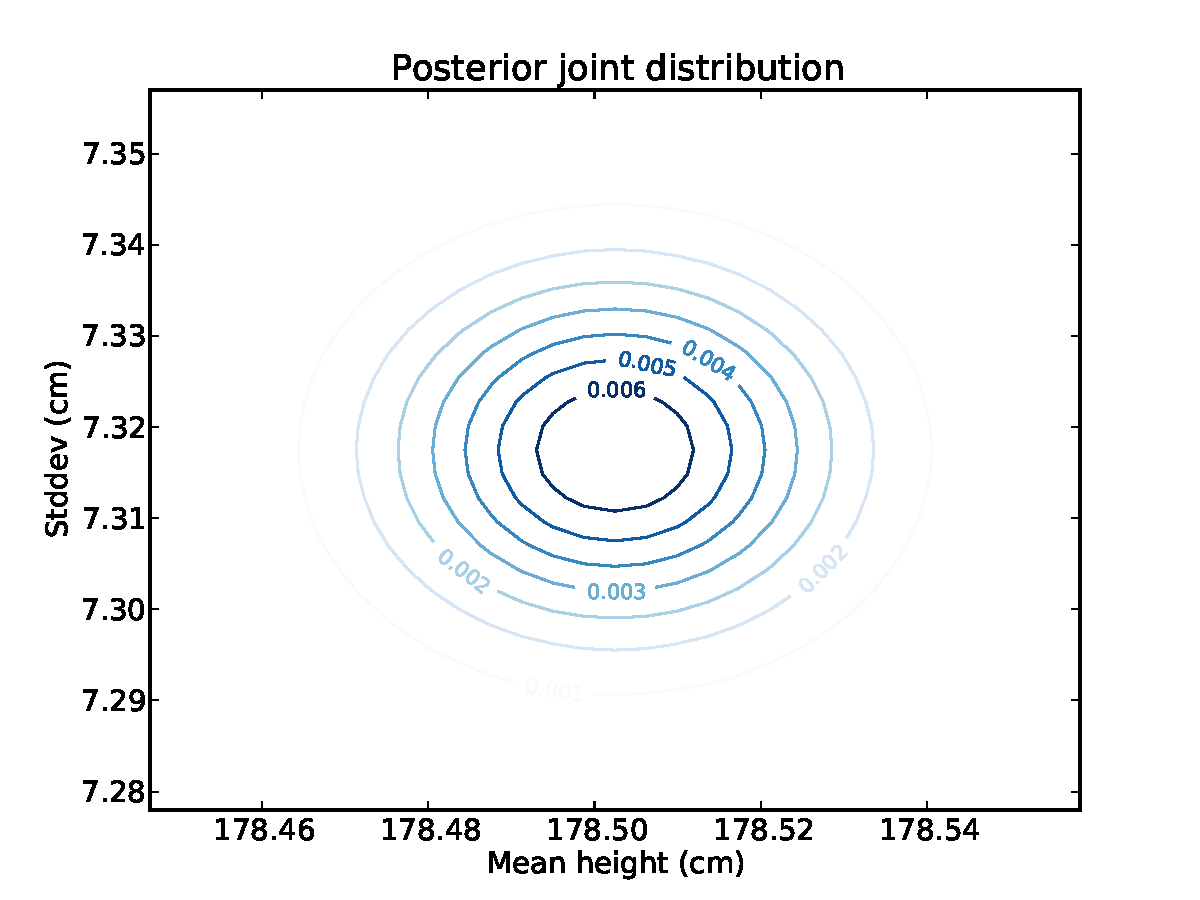
\includegraphics[height=2.5in]{figs/variability_posterior_male.pdf}}
\caption{Contour plot of the posterior joint distribution of
mean and standard deviation of height for men in the U.S.}
\label{fig.variability1}
\end{figure}

\begin{figure}
% variability.py
\centerline{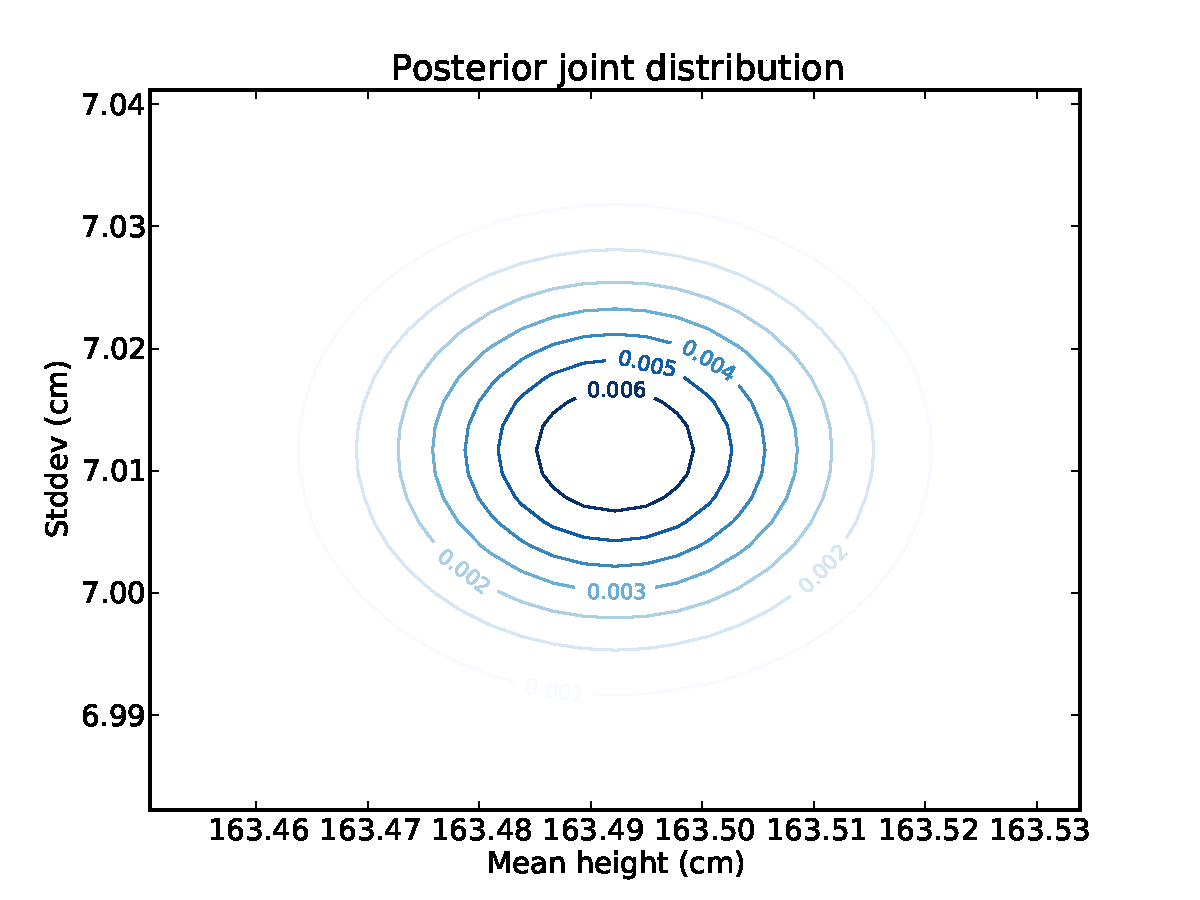
\includegraphics[height=2.5in]{figs/variability_posterior_female.pdf}}
\caption{Contour plot of the posterior joint distribution of
mean and standard deviation of height for women in the U.S.}
\label{fig.variability2}
\end{figure}

We are almost ready to look at results, but we have one more
problem to deal with.  There are a number of outliers in this
dataset that are almost certainly errors.  For example, there
are three adults with reported height of 61 cm, which would
place them among the shortest living adults in the world.
At the other end, there are four women with reported height
229 cm, just short of the tallest women in the world.

It is not impossible that these values are correct, but it is
unlikely, which makes it hard to know how to deal with them.
But since we are trying to estimate variability, we have to get
it right, since these extreme values have a disproportionate
effect on the estimates.

Because ABC is based on summary statistics, rather than the entire
data set, we can make it more robust by choosing summary statistics
that are robust in the presence of outliers.  Specifically, rather
than use the sample mean and standard deviation, we can use the median
and an inter-percentile range.  For example, the inter-quartile range
(IQR) is the difference between the 25th and 75th percentiles.

More generally, we can compute an inter-percentile range that
spans a given fraction of the distribution, {\tt p}:

\begin{verbatim}
def MedianIPR(xs, p=0.6827):
    cdf = thinkbayes.MakeCdfFromList(xs)
    median = cdf.Percentile(50)

    alpha = (1-p) / 2
    ipr = cdf.Value(1-alpha) - cdf.Value(alpha)
    return median, ipr
\end{verbatim}

The result is the median and the inter-percentile range.  We can
convert from {\tt ipr} to an estimate of {\tt sigma} using the
Gaussian CDF to compute the fraction of the distribution covered by a
given number of standard deviations.  For example, it is a well-known
rule of thumb that 68\% of a Gaussian distribution falls within one
standard deviation of the mean, which leaves 16\% in each tail.  If
we compute the range between the 16th and 84th percentiles, we expect
the result to be {\tt 2 * sigma}.  So we can estimate {\tt sigma}
by computing the 68\% IPR and dividing by 2.

The following function does the same computation for any number of
sigmas:

\begin{verbatim}
def MedianSighat(xs, num_sigmas):
    half_p = thinkbayes.StandardGaussianCdf(num_sigmas) - 0.5

    median, ipr = MedianIPR(xs, half_p * 2)
    sighat = ipr / 2 / num_sigmas

    return median, sighat
\end{verbatim}

The result is an estimate of {\tt sigma}, which I call {\tt sighat}
because ``hat'' is the conventional symbol that indicates an
estimate.

Then in {\tt LogUpdateSetABC} we can replace the
conventional estimators, {\tt xbar} and {\tt S}, with {\tt median}
and {\tt sighat}.  And that pretty much does it.

It might seem odd that we are using observed percentiles to
estimate {\tt mu} and {\tt sigma}, but it is an example of the
flexibility of the Bayesian approach.  In effect we are asking,
``Given hypothetical values for {\tt mu} and {\tt sigma}, and
a sampling process that has some chance of introducing errors,
what is the likelihood of generating a given set of sample
statistics?''

We are free to choose any sample statistics we like, up to a point:
{\tt mu} and {\tt sigma} determine the location and spread of
a distribution, so we need to choose statistics that capture those
characteristics.  For example, if we chose the 49th and 51st percentiles,
we would get very little information about spread, so it
would leave the estimate of {\tt sigma} relatively unconstrained
by the data.  All values of {\tt sigma} would have nearly the
same likelihood of producing the observed values, so the posterior
marginal distribution for {\tt sigma} would look a lot like the
prior.


\section{Who is more variable?}

\begin{figure}
% variability.py
\centerline{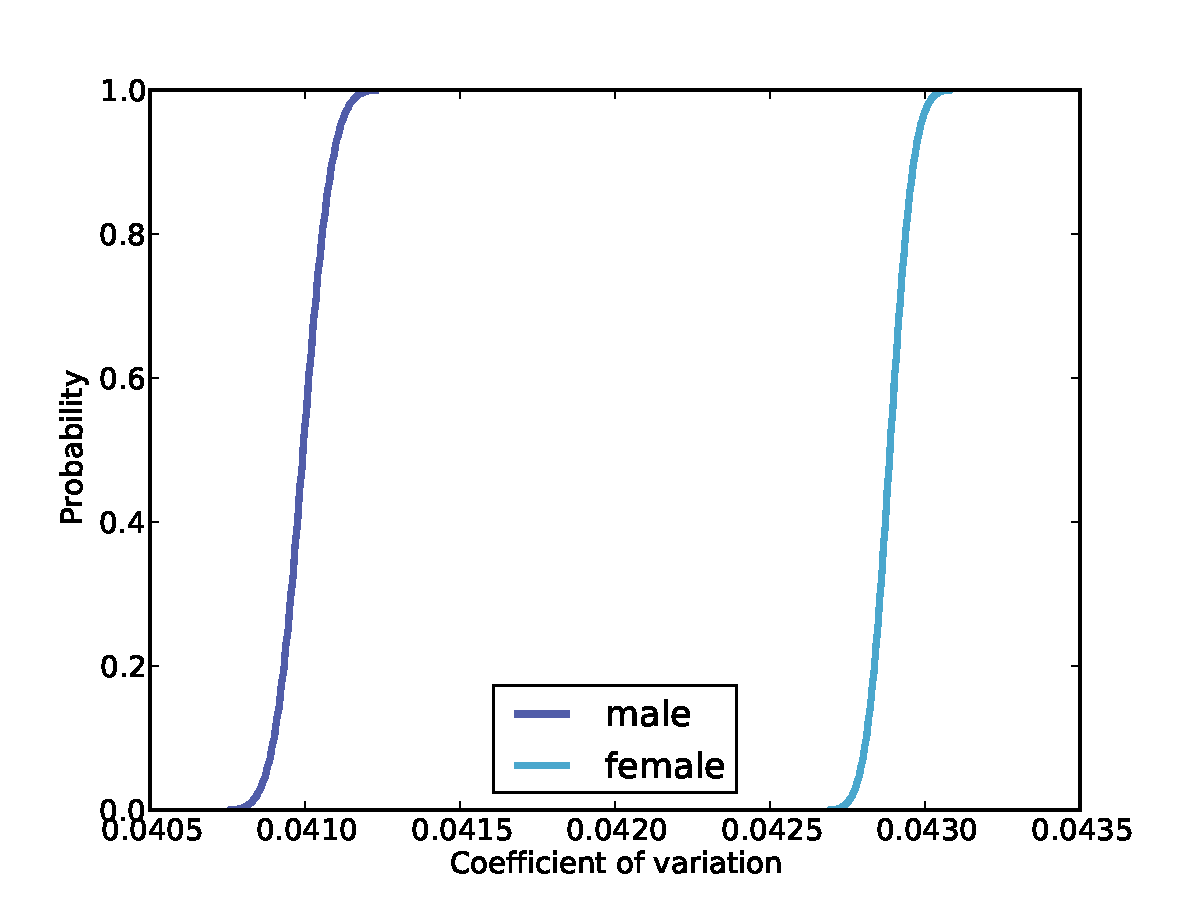
\includegraphics[height=2.5in]{figs/variability_cv.pdf}}
\caption{Contour plot of the posterior joint distribution of
mean and standard deviation of height for women in the U.S.}
\label{fig.variability3}
\end{figure}

Finally we are ready to answer the question we started with: is the
coefficient of variation greater for men than for women?

Using ABC based on the median and IPR with \verb"num_sigmas=1", I
computed posterior joint distributions for {\tt mu} and {\tt
  sigma}.  Figures~\ref{fig.variability1} and ~\ref{fig.variability2}
show the results as a contour plot with {\tt mu} on the x-axis, {\tt
  sigma} on the y-axis, and probability on the z-axis.

The most likely values for men are 178 cm and 7.4 cm, so the
maximum likelihood estimate for {\tt sigma}, based on robust
sample statistics, is a bit less than the observed
standard deviation, 7.7 cm.

For women, the most likely values are 163 cm and 7.0 cm.  Again,
the estimate of {\tt sigma} is less than the observed
standard deviation, 7.3 cm.

For each joint distribution, we compute the posterior distribution of
CV.  Figure~\ref{fig.variability3} shows these distributions for men
and women.  The mean for men is 0.0410; for women it is 0.0429.  And
since there is no overlap between the distributions, we conclude that
women are more variable in height than men.

So is that the end of the Variability Hypothesis?  Sadly, no.  This
result turns out to depend strongly on the choice of the
inter-percentile range.  With \verb"num_sigmas=1", we conclude that
women are more variable, but with \verb"num_sigmas=2" we conclude
with equal confidence that men are more variable.

The reason for the difference is that there are differences in the
shapes of the distributions for men and women.  Specifically, there
are more men of short stature, and their distance from the mean is
greater.

So our evaluation of the Variability Hypothesis depends on the
interpretation of ``variability.''  With \verb"num_sigmas=1" we are
measuring differences between people within one standard deviation of
the mean, people we would call ``normal'' for want of less value-laden
word.  As we increase \verb"num_sigmas", the measure of variability is
influenced by an increasing number of people whose stature is affected
by medical conditions.  How much effect these people should have
on the result depends on what notion of variability we are trying
to capture, which depends on theory we are trying to test.

In the case of the Variability Hypothesis, I don't think the theory
is sufficiently well-defined to test, and even if it were, I don't
think the results would mean very much.

I hope you agree that this example is interesting, and it helped
me demonstrate several new ideas, but at this point we have probably
given the Variability Hypothesis more energy than it deserves, so
let's stop there.

You can download the code in this chapter from
\url{http://thinkbayes.com/variability.py}.


\section{Exercises}

\begin{exercise}

Cohen's $d$ is a statistic that measures the size of the difference in
means between two groups (see
\url{http://en.wikipedia.org/wiki/Effect_size}).  It is defined as
%
\[ \frac{\bar{x}_1 - \bar{x}_2}{s} \]
%
where $\bar{x}_1$ is the sample mean of the first group, $\bar{x}_2$
is the sample mean of the second group, and $s$ is the estimated
pooled standard deviation for the two groups (you can look up the
formula).

Write a function that takes the posterior distributions for
the mean and standard deviation of height and computes the
posterior distribution of Cohen's $d$.

Hint: instead of enumerating all possible values of $\mu$ and
$\sigma$ for men and women, you might want to draw a random sample
from the posterior distributions.

\end{exercise}



\chapter{Hypothesis testing}

\section{Back to the Euro problem}

In Section~\ref{euro} I presented a question from MacKay's {\it Information
  Theory, Inference, and Learning Algorithms}:

\begin{quote}
A statistical statement appeared in ``The Guardian" on Friday January 4, 2002:

  \begin{quote}
        When spun on edge 250 times, a Belgian one-euro coin came
        up heads 140 times and tails 110.  `It looks very suspicious
        to me,' said Barry Blight, a statistics lecturer at the London
        School of Economics.  `If the coin were unbiased, the chance of
        getting a result as extreme as that would be less than 7\%.'
        \end{quote}

But do these data give evidence that the coin is biased rather than fair?
\end{quote}

We used this data to estimate the probability that the coin would
land face up, but we didn't really answer MacKay's question.  Let's
get back to that now.

\section{Bayesian hypothesis testing}

In Section~\ref{oliver} I proposed that data are in favor of
a hypothesis if the data are more likely under the hypothesis than
under the alternative or, equivalently, if the Bayes factor is greater
than 1.

In the Euro example, we have two hypotheses to consider: I'll use
$F$ for the hypothesis that the coin is fair and $B$ for the hypothesis
that it is biased.

If the coin is fair, it is easy to compute the likelihood of the
data, \p{D|F}.  In fact, we already wrote the {\tt Likelihood}
that does it.

\begin{verbatim}
    def Likelihood(self, hypo, data):
        x = hypo / 100.0
        head, tails = data
        like = x**heads * (1-x)**tails
        return like
\end{verbatim}

All we have to do is create a {\tt Euro} suite and use its 
{\tt Likelihood} method:

\begin{verbatim}
    suite = Euro()
    likelihood = suite.Likelihood(50, data)
\end{verbatim}

\p{D|F} is $5.5 \cdot 10^{-76}$, which doesn't tell us much except
that the probability of seeing any particular dataset is very small.
As always, it takes two likelihoods to make a ratio, so we have to
compute \p{D|B}.

It is not obvious how to compute the likelihood of $B$, because
it's not obvious what ``biased'' means.

One possibility is to cheat and look at the data before we define
the hypothesis.  In that case we would say that ``biased'' means that
the probability of heads is 140/250.

\begin{verbatim}
    actual_percent = 100.0 * 140 / 250
    likelihood = suite.Likelihood(actual_percent, data)
\end{verbatim}

This version of $B$ I call \verb"B_cheat"; the likelihood of
\verb"b_cheat" is $34 \cdot 10^{-76}$ and the likelihood ratio is
6.1.  So we would say that the data are evidence in favor of this
version of $B$.

But using the data to formulate the hypothesis
is obviously bogus.  By that definition, any dataset would
be evidence in favor of $B$, unless the observed percentage of heads
is exactly 50\%.

\section{Making a fair comparison}

To make a legitimate comparison, we have to define $B$ without looking
at the data.  So let's try a different definition.  If you inspect
a Belgian Euro coin, you might notice that the ``heads'' side is more
prominent than the ``tails'' side.  You might expect the shape to 
have some effect on
$x$, but be unsure whether it makes heads more or less
likely.  So you might say ``I think the coin is biased so that
$x$ is either 0.6 or 0.4, but I am not sure which.''

We can think of this version, which I'll call \verb"B_two"
as a hypothesis made up of two
sub-hypotheses.  We can compute the likelihood for each
sub-hypothesis and then compute the average likelihood.

\begin{verbatim}
    like40 = suite.Likelihood(40, data)
    like60 = suite.Likelihood(60, data)
    likelihood = 0.5 * like40 + 0.5 * like60
\end{verbatim}

The likelihood ratio (or Bayes factor) for \verb"b_two" is 1.3, which
means the data provide weak evidence in favor of \verb"b_two".

More generally, suppose you suspect that the coin is biased,
but you have no clue about the value of $x$.  In that case you
might build a Suite to represent sub-hypotheses from 0 to 100.

\begin{verbatim}
    b_uniform = Euro(xrange(0, 101))
    b_uniform.Remove(50)
    b_uniform.Normalize()
\end{verbatim}

I removed the sub-hypothesis that $x$ is 50\%, but it doesn't
really matter if you include it.  To compute the likelihood of
\verb"b_uniform" we compute the likelihood of the sub-hypotheses
and compute a weighted average.

\begin{verbatim}
def SuiteLikelihood(suite, data):
    total = 0
    for hypo, prob in suite.Items():
        like = suite.Likelihood(hypo, data)
        total += prob * like
    return total
\end{verbatim}

The likelihood ratio for \verb"b_uniform" is 0.47, which means
that the data are weak evidence against \verb"b_uniform" at
least compared to $F$.

If you think about the computation performed by
\verb"SuiteLikelihood", you might notice that it is similar to an
update.  To refresh your memory, here's the {\tt Update} function:

\begin{verbatim}
    def Update(self, data):
        for hypo in self.Values():
            like = self.Likelihood(hypo, data)
            self.Mult(hypo, like)
        return self.Normalize()
\end{verbatim}

And here's {\tt Normalize}:

\begin{verbatim}
    def Normalize(self):
        total = self.Total()
        
        factor = 1.0 / total
        for x in self.d:
            self.d[x] *= factor

        return total
\end{verbatim}

The return value from {\tt Normalize} is the total of the probabilities
in the Suite, which is the average of the likelihoods for the
sub-hypotheses, weighted by the prior probabilities.  And {\tt Update}
passes this value along, so we could compute the likelihood
of \verb"b_uniform" like this:

\begin{verbatim}
    likelihood = b_uniform.Update(data)
\end{verbatim}



\section{The triangle prior}

In Chapter~\ref{euro} we also considered a triangle-shaped prior that
gives higher probability to values of $x$ near 50\%.  If we think of
this prior as a suite of sub-hypotheses, we can compute its likelihood
like this:

\begin{verbatim}
    b_triangle = TrianglePrior()
    likelihood = b_triangle.Update(data)
\end{verbatim}

{\tt TrianglePrior} is defined in Section~\ref{triangle} and
shown in Figure~\ref{fig.euro2}.

The likelihood ratio for \verb"b_triangle" is 0.84, compared to $F$, so
again we would say that the data are weak evidence against $B$.

The following table shows the different priors we have considered, the
likelihood of each, and the likelihood ratio (or Bayes factor)
relative to $F$.

\begin{tabular}{|l|r|r|}
\hline
Hypothesis   & Likelihood & Bayes  \\
             & $\times 10^{-76}$ & Factor  \\
\hline
$F$              & 5.5   & --   \\
\verb"B_cheat"  & 34   &  6.1   \\
\verb"B_two"     & 7.4   &  1.3   \\
\verb"B_uniform"  & 2.6   &  0.47   \\
\verb"B_triangle"  & 4.6   &  0.84   \\
\hline
\end{tabular}

In summary, we can use Bayesian hypothesis testing to compare the
likelihood of $F$ and $B$, but we have to do some work to specify
precisely what $B$ means.  This specification depends on background
information about coins and their behavior when spun, so people
could reasonably disagree about the ``right'' definition.

Depending on which definition we choose, the data might provide
evidence for or against the hypothesis that the coin is biased, but
in either case it is relatively weak evidence.

I should acknowledge that my presentation of this example follows
David MacKay's discussion, and comes to the same conclusion.

You can download the code I used in this chapter from
\url{http://thinkbayes.com/euro3.py}.


\section{Strength of evidence}

The Bayes factor for \verb"B_uniform" is 0.47, which means
that the data provide evidence against this hypothesis (compared
to $F$).  In the previous section I characterized this evidence
as ``weak,'' but I didn't say why.

Part of the answer is historical.  Harold Jeffreys, an early
proponent of Bayesian statistics, suggested a scale for
interpreting Bayes factors:

\begin{tabular}{|l|l|}
\hline
Bayes & Strength \\
Factor & \\
\hline
1 -- 3 & Barely worth mentioning \\
3 -- 10 & Substantial \\
10 -- 30 & Strong \\
30 -- 100 & Very strong \\
$>$ 100 & Decisive \\
\hline
\end{tabular}

In the example, the Bayes factor is 0.47 in favor of \verb"B_uniform",
so it is 2.1 in favor is $F$, which Jeffreys would consider
``barely worth mentioning.''

Other authors have suggested variations on the wording.  To
avoid arguing about adjectives, we could think about odds instead.

If your prior odds are 1:1, and you see evidence with Bayes
factor 2, your posterior odds are 2:1.  In terms of probability,
the data changed your degree of belief from 50\% to 66\%.  For
most real world problems, that change would be small relative
to the uncertainty of the prior.

On the other hand, if you had seen evidence with Bayes
factor 100, your posterior odds would be 100:1 or more than 99\%.
Whether or not you agree that such evidence is ``decisive,''
it is certainly strong.

\begin{exercise}
Some people believe in the existence of extra-sensory
perception (ESP); for example, the ability of some people to guess
the value of an unseen playing card with probability better
than chance.

What is your prior degree of belief in this kind of ESP?
Do you think it is as likely to exist as not?  Or are you
more skeptical about it?  Write down your prior odds.

Now compute the strength of the evidence it would take to
convince you that ESP is at least 50\% likely to exist.
What Bayes factor would be needed to make you 90\% sure
that ESP exists?
\end{exercise}


\begin{exercise}
Suppose that your answer to the previous question is 1000;
that is, evidence with Bayes factor 1000 in favor of ESP would
be sufficient to change your mind.

Now suppose that you read a paper in a respectable peer-reviewed
scientific journal that presents evidence with Bayes factor 1000 in
favor of ESP.  Would that change your mind?

If not, how do you resolve the apparent contradiction?
You might find it helpful to read about David Hume's article, ``Of
Miracles,'' at \url{http://en.wikipedia.org/wiki/Of_Miracles}.
\end{exercise}



\chapter{Evidence}
\label{evidence}

\section{Interpreting SAT scores}

Suppose you are the Dean of Admission at a small engineering
college in Massachusetts, and you are considering two candidates,
Alice and Bob, whose qualifications are similar in many ways,
with the exception that Alice got a higher score on the Math
portion of the SAT, a standardized test intended to measure
preparation for college-level work in mathematics.

If Alice got 780 and Bob got a 740 (out of a possible 800), you might
want to know whether that difference is evidence that Alice is better
prepared than Bob, and what the strength of that evidence is.

Now in reality, both scores are very good, and both 
candidates are probably well prepared for college math.  So
the real Dean of Admission would probably suggest that we choose
the candidate who best demonstrates the other skills and
attitudes we look for in students.  But as an example of
Bayesian hypothesis testing, let's stick with a narrower question:
``How strong is the evidence that Alice is better prepared
than Bob?''

To answer that question, we need to make some modeling decisions.
I'll start with a simplification I know is wrong; then we'll come back
and improve the model.  Specifically, I will temporarily pretend that
all SAT questions are equally difficult.  In reality, the designers of
the SAT choose questions with a range of difficulty, because that
improves the ability to measure statistical differences between
test-takers.

But if we choose a model where all questions are equally difficult, we
can define a characteristic, \verb"p_correct", for each test-taker,
which is the probability of answering any question correctly.  This
simplification makes it easy to compute the likelihood of a given
score.


\section{The scale}

In order to understand SAT scores, we have to understand the scoring
and scaling process.  Each test-taker gets a raw score based on the
number of correct and incorrect questions.  The raw score is converted
to a scaled score in the range 200--800.

In 2009, there were 54 questions on the math SAT.  The raw score
for each test-taker is the number of questions answered correctly
minus a penalty of $1/4$ point for each question answered incorrectly.

The College Board, which administers the SAT, publishes the
mapping from raw scores to scaled scores.  I have downloaded that
data and wrapped it in an Interpolator object that provides a forward
lookup (from raw score to scaled) and a reverse lookup (from scaled
score to raw).

You can download the code for this example from
\url{http://thinkbayes.com/sat.py}.


\section{The prior}

The College Board also publishes the distribution of scaled scores
for all test-takers.  If we convert each scaled score to a raw score,
and divide by the number of questions, the result is an estimate
of \verb"p_correct".
So we can use the distribution of raw scores to model the
prior distribution of \verb"p_correct".

Here is the code that reads and processes the data:

\begin{verbatim}
class Exam(object):

    def __init__(self):
        self.scale = ReadScale()
        scores = ReadRanks()
        score_pmf = thinkbayes.MakePmfFromDict(dict(scores))
        self.raw = self.ReverseScale(score_pmf)
        self.prior = DivideValues(raw, 54)
\end{verbatim}

{\tt Exam} encapsulates the information we have about the offering
of an exam.
{\tt ReadScale} and {\tt ReadRanks} read files and return
object that contain the data:
{\tt self.scale} is the {\tt Interpolator} that converts
from raw to scaled scores and back;  {\tt scores} is a list
of (score, frequency) pairs.

\verb"score_pmf" is the Pmf of
scaled scores.   {\tt raw} is the Pmf of raw scores, and
{\tt self.prior} is the Pmf of \verb"p_correct".

\begin{figure}
% sat.py
\centerline{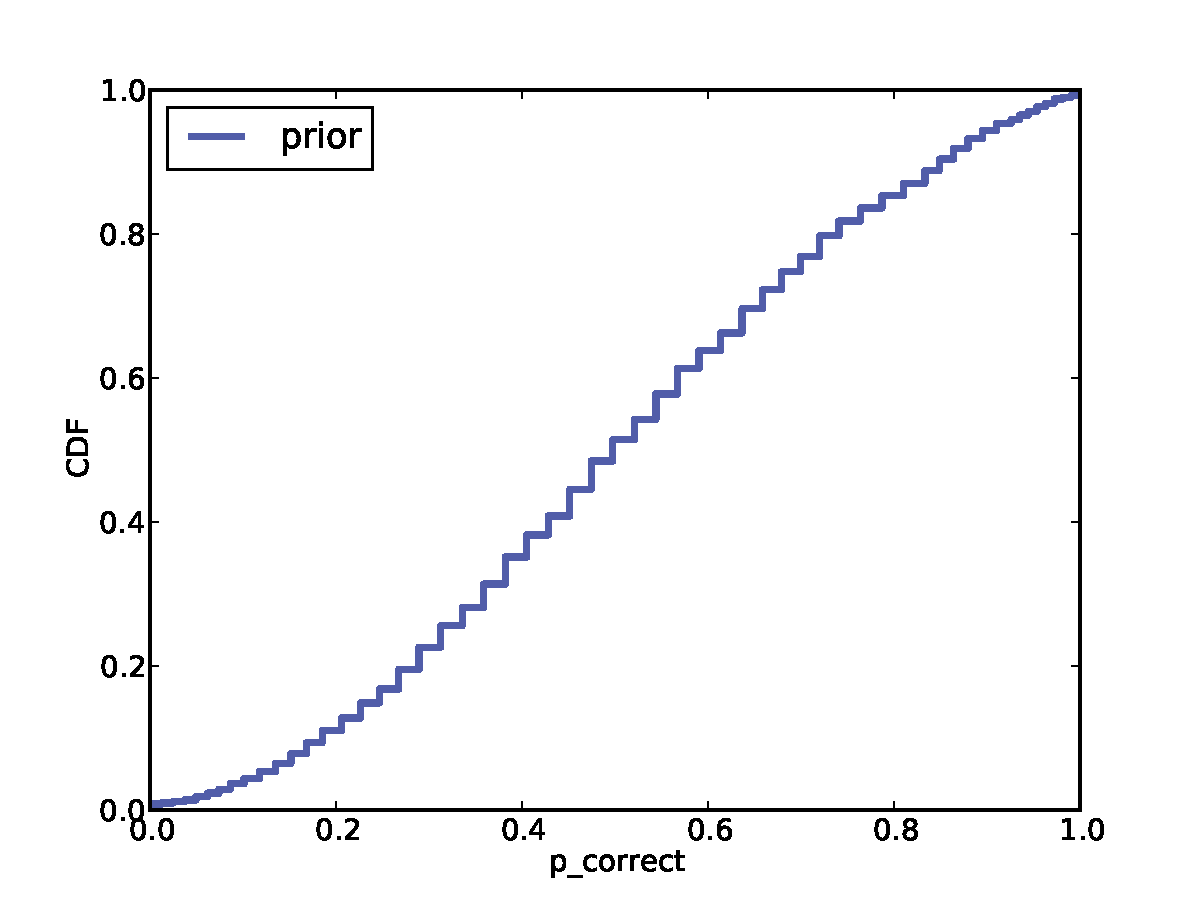
\includegraphics[height=2.5in]{figs/sat_prior.pdf}}
\caption{Prior distribution of {\tt p\_correct} for SAT test-takers.}
\label{fig.satprior}
\end{figure}

Figure~\ref{fig.satprior} shows the prior distribution of
\verb"p_correct".  This distribution is approximately normal, but it
is compressed at the extremes.  By design, the SAT has the most power
to discriminate between test-takers within two standard deviations of
the mean, and less power outside that range.

For each test-taker, I define a Suite called {\tt Sat} that
represents the distribution of \verb"p_correct".  Here's the definition:

\begin{verbatim}
class Sat(thinkbayes.Suite):

    def __init__(self, exam, score):
        thinkbayes.Suite.__init__(self)

        self.exam = exam
        self.score = score

        # start with the prior distribution
        for p_correct, prob in exam.prior.Items():
            self.Set(p_correct, prob)

        # update based on an exam score
        self.Update(score)
\end{verbatim}

\verb"__init__" takes an Exam object and a scaled score.  It makes a
copy of the prior distribution and then updates itself based on the
exam score.

As usual, we inherit {\tt Update} from {\tt Suite} and provide
{\tt Likelihood}:

\begin{verbatim}
    def Likelihood(self, hypo, data):
        p_correct = hypo
        score = data

        raw = self.exam.Reverse(score)
        yes, no = raw, 54 - raw

        like = thinkbayes.EvalBinomialPmf(p_correct, yes, no)
        return like
\end{verbatim}

And as usual, {\tt Likelihood} computes the likelihood of the data
under a given hypothesis.  In this case {\tt hypo} is a hypothetical
value of \verb"p_correct".  And {\tt data} is a scaled score.

To keep things simple, I interpret the raw score as the number of
correct answers, ignoring the penalty for wrong answers.  With
this simplification, the likelihood is given by the binomial
distribution, which computes the probability of {\tt yes} correct
answers and {\tt no} incorrect.


\section{Posterior}

\begin{figure}
% sat.py
\centerline{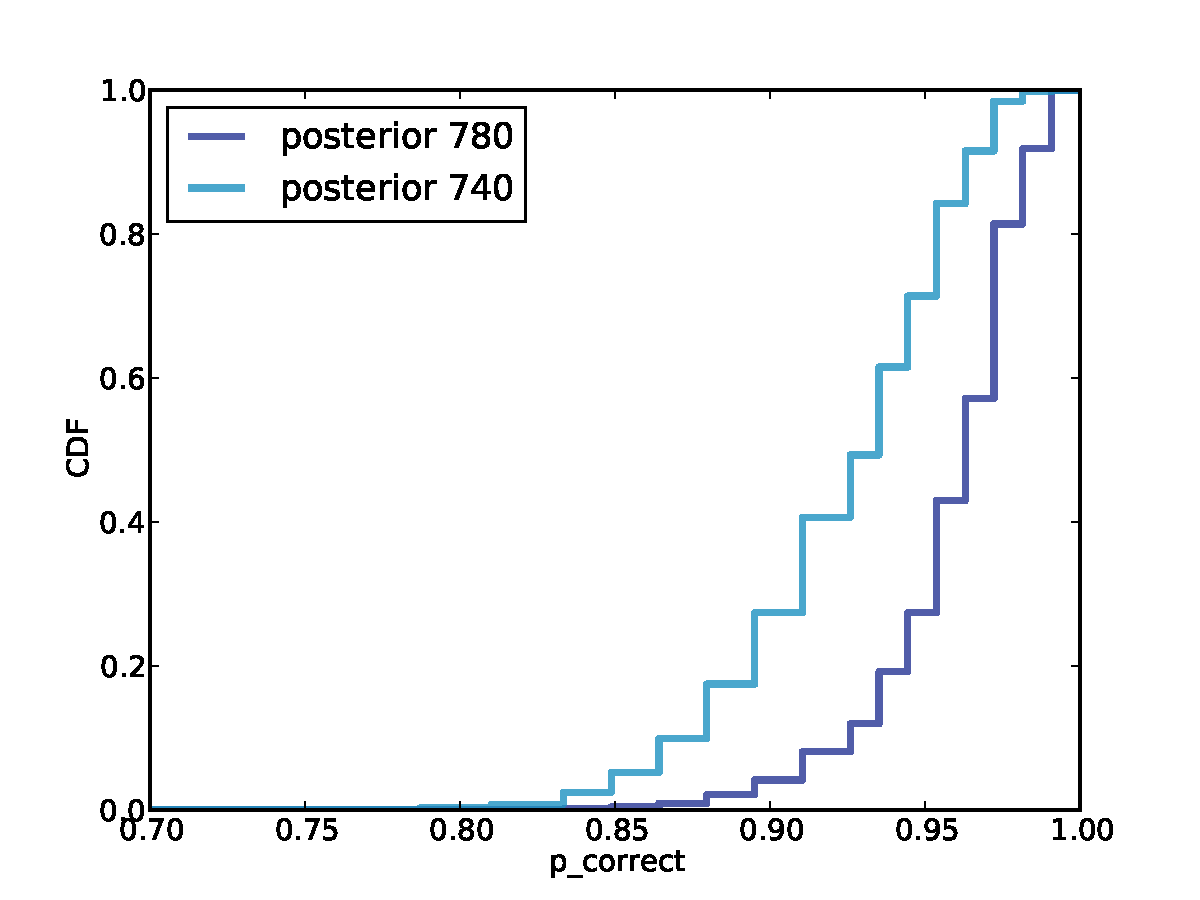
\includegraphics[height=2.5in]{figs/sat_posteriors_p_corr.pdf}}
\caption{Posterior distributions of {\tt p\_correct} for Alice and Bob.}
\label{fig.satposterior1}
\end{figure}

Figure~\ref{fig.satposterior1} shows the posterior distributions
of \verb"p_correct" for Alice and Bob based on their exam scores.
We can see that they overlap, so it is possible that \verb"p_correct"
is actually higher for Bob, but it looks unlikely.

Which brings us back to the original question, ``How strong is the
evidence that Alice is better prepared than Bob?''  We can use the
posterior distributions of \verb"p_correct" to answer this question.

To formulate the question in terms of Bayesian hypothesis testing,
I define two hypotheses:

\begin{itemize}

\item A: \verb"p_correct" is higher for Alice than for Bob.

\item B: \verb"p_correct" is higher for Bob than for Alice.

\end{itemize}

To compute the likelihood of A, we can enumerate all pairs of values
from the posterior distributions, and add up the total probability of
the cases where \verb"p_correct" is higher for Alice than for Bob.
And we already have a function, \verb"thinkbayes.PmfProbGreater"
that does that.

So we can define a Suite that computes the posterior probabilities
of $A$ and $B$:

\begin{verbatim}
class TopLevel(thinkbayes.Suite):

    def Update(self, data):
        a_sat, b_sat = data

        a_like = thinkbayes.PmfProbGreater(a_sat, b_sat)
        b_like = thinkbayes.PmfProbLess(a_sat, b_sat)
        c_like = thinkbayes.PmfProbEqual(a_sat, b_sat)

        a_like += c_like / 2
        b_like += c_like / 2

        self.Mult('A', a_like)
        self.Mult('B', b_like)

        self.Normalize()
\end{verbatim}

Usually when we define a new Suite, we inherit {\tt Update}
and provide {\tt Likelihood}.  In this case I override {\tt Update},
because it is easier to evaluate the likelihood of both
hypotheses at the same time.

The data passed to {\tt Update} are Sat objects that represent
the posterior distributions of \verb"p_correct".

\verb"a_like" is the total probability that
\verb"p_correct" is higher for Alice; \verb"b_like" is that
probability that it is higher for Bob.

\verb"c_like" is the probability that they are ``equal,'' but this
equality is an artifact of the decision to model \verb"p_correct" with
a set of discrete values.  If we chose more values, \verb"c_like"
would be smaller, and in the extreme, if \verb"p_correct" were
continuous, \verb"c_like" would be zero.  So I treat \verb"c_like" as
a kind of round-off error, and split it evenly between \verb"a_like"
and \verb"b_like".

Here is the code that creates {\tt TopLevel} and updates it:

\begin{verbatim}
    exam = Exam()
    a_sat = Sat(exam, 780)
    b_sat = Sat(exam, 740)

    top = TopLevel('AB')
    top.Update((a_sat, b_sat))
    top.Print()
\end{verbatim}

The likelihood of $A$ is 0.79 and the likelihood of $B$ is 0.21.  The
likelihood ratio (or Bayes factor) is 3.8, which means that these test
scores are evidence that Alice is better than Bob at answering SAT
questions.  If we believed, before seeing the test scores, that $A$
and $B$ were equally likely, then after seeing the scores we should
believe that the probability of $A$ is 79\%, which means there is
still an 21\% chance that Bob is actually better prepared.


\section{A better model}

Remember that the analysis we have done so far is based on
the simplification that all SAT questions are equally difficult.
In reality, some are easier than others, which means that the
difference between Alice and Bob might be even smaller.

To see why, consider a test where most questions are so easy that
Alice and Bob are nearly certain to answer them correctly.  In that
case, the difference between their scores is determined by a small
number of difficult questions, so it is more likely to be due to
chance.

But how big is the modeling error?  If it is small, we conclude
that the first model---based on the simplification that all questions
are equally difficult---is good enough.  If it's large,
we need a better model.

In the next few sections, I develop a better model and we will
discover (spoiler alert!) that the modeling error is small.  So if
you are satisfied with the simpler mode, you can skip to the next
chapter.  If you want to see how the more realistic model works,
read on...

\begin{itemize}

\item First, let's assume that each test-taker has some 
  degree of {\tt efficacy}, that measures their
  ability to answer SAT questions.

\item Second, assume that each question has some level of
  {\tt difficulty}.

\item Finally, assume that the chance that a test-taker answers a
  question correctly is related to {\tt efficacy} and {\tt difficulty}
  according to this function:

\begin{verbatim}
def ProbCorrect(efficacy, difficulty, a=1):
    return 1 / (1 + math.exp(-a * (efficacy - difficulty)))
\end{verbatim}

\end{itemize}

This function is a simplified version of the curve used in item
response theory, which you can read about at
\url{http://en.wikipedia.org/wiki/Item_response_theory}.  {\tt
  efficacy} and {\tt difficulty} are considered to be on the same
scale, and the probability of getting a question right depends only on
the difference between them.

When {\tt efficacy} and {\tt difficulty} are equal, the
probability of getting the question right is 50\%.  As
{\tt efficacy} increases, this probability approaches 100\%.
As it decreases (or as {\tt difficulty} increases), the
probability approaches 0\%.

Given the distribution of {\tt efficacy} across test-takers
and the distribution of {\tt difficulty} across questions, we
can compute the expected distribution of raw scores.  We'll do that
in two steps.  First, for a person with given {\tt efficacy},
we'll compute the distribution of raw scores.

\begin{verbatim}
def PmfCorrect(efficacy, difficulties):
    pmf0 = thinkbayes.Suite([0])

    ps = [ProbCorrect(efficacy, diff) for diff in difficulties]
    pmfs = [BinaryPmf(p) for p in ps]
    dist = sum(pmfs, pmf0)
    return dist
\end{verbatim}

{\tt difficulties} is a list of difficulties, one for each question.
{\tt ps} is a list of probabilities, and {\tt pmfs} is a list of
two-valued Pmf objects; here's the function that makes them:

\begin{verbatim}
def BinaryPmf(p):
    pmf = thinkbayes.Pmf()
    pmf.Set(1, p)
    pmf.Set(0, 1-p)
    return pmf
\end{verbatim}

{\tt dist} is the sum of these Pmfs.  Remember from Section~\ref{addends}
that when we add up Pmf objects, the result is the distribution
of the sums.  In order to use Python's {\tt sum} to add up Pmfs,
we have to provide {\tt pmf0} which is the identity for Pmfs,
so {\tt pmf + pmf0} is always {\tt pmf}.

So if we know a person's efficacy, we can compute their distribution
of raw scores.  For a group of people with a different efficacies, the
resulting distribution of raw scores is a mixture.  Here's the code
that computes the mixture:

\begin{verbatim}
class Exam:

    def MakeRawScoreDist(self, efficacies):
        pmfs = thinkbayes.Pmf()
        for efficacy, prob in efficacies.Items():
            scores = PmfCorrect(efficacy, self.difficulties)
            pmfs.Set(scores, prob)

        mix = thinkbayes.MakeMixture(pmfs)
        return mix
\end{verbatim}

{\tt efficacies} is a Pmf that represents the distribution of efficacy
across test-takers.  I assume that it is Gaussian with mean 0 and
standard deviation 1.5.  This choice is mostly arbitrary.  The
probability of getting a question correct depends on the difference
between efficacy and difficulty, so we can choose the units of
efficacy and then calibrate the units of difficulty accordingly.

{\tt pmfs} is a Meta-Pmf that contains one Pmf for each level of
efficacy, and maps to the fraction of test-takers at that level.  {\tt
  thinkbayes.MakeMixture} takes the meta-pmf and compute the
distribution of the mixture (see Section~\ref{meta-pmf}).


\section{Calibration}

If we were given the distribution of difficulty, we could use
\verb"MakeRawScoreDist" to compute the distribution of raw scores.
But for us the problem is the other way around: we are given the
distribution of raw scores and we want to infer the distribution of
difficulty.

\begin{figure}
% sat.py
\centerline{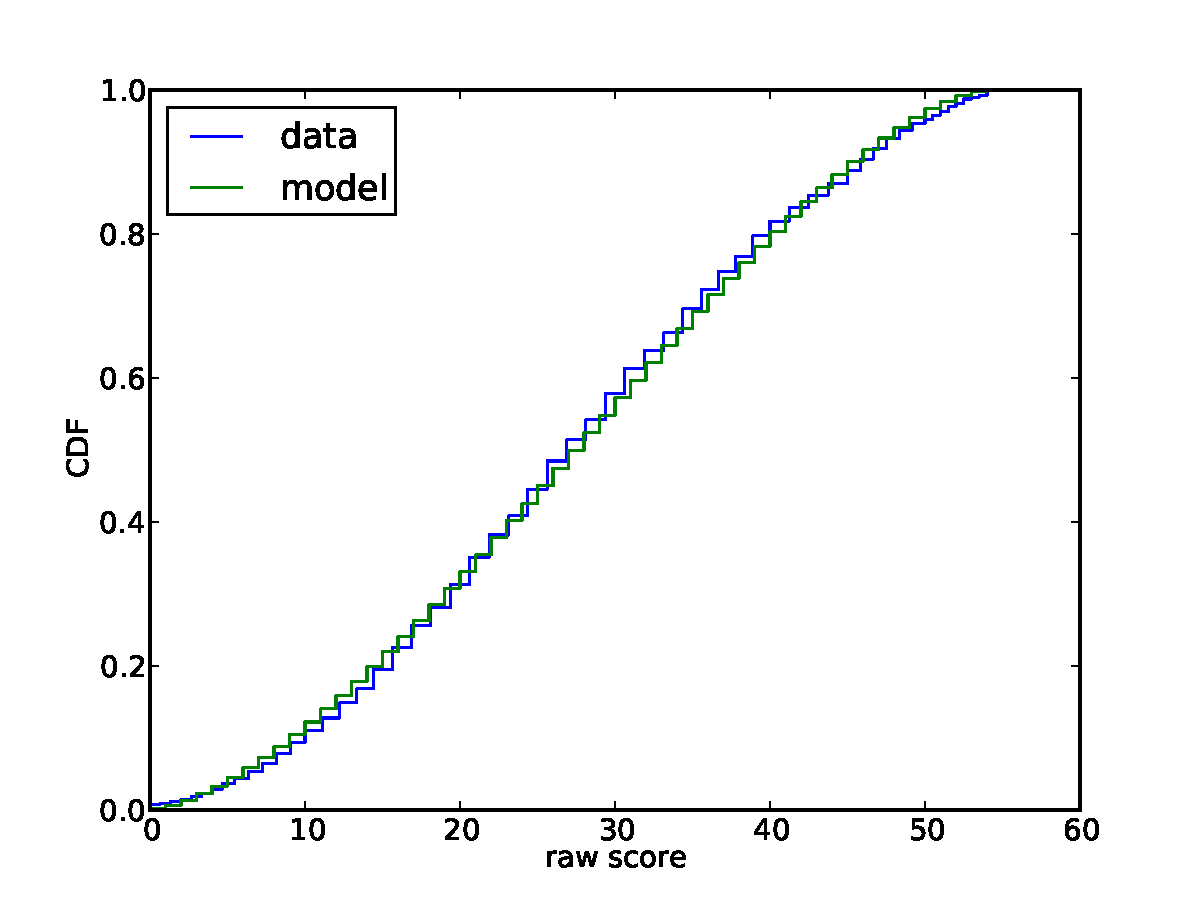
\includegraphics[height=2.5in]{figs/sat_calibrate.pdf}}
\caption{Actual distribution of raw scores and a model to fit it.}
\label{fig.satcalibrate}
\end{figure}

I assume that the distribution of difficulty is uniform with
parameters {\tt center} and {\tt width}.  {\tt MakeDifficulties}
makes a list of difficulties with these parameters.

\begin{verbatim}
def MakeDifficulties(center, width, n):
    low, high = center-width, center+width
    return numpy.linspace(low, high, n)
\end{verbatim}

By trying out a few combinations, I found that
the values {\tt center=-0.05} and {\tt width=1.8} yield a distribution
of raw scores similar to the actual data.
Figure~\ref{fig.satcalibrate} shows the actual data and the results
from this model.

So, assuming that the distribution of difficulty is uniform,
the range is approximately
{\tt -1.85} to {\tt 1.75}, on a scale with a distribution of
efficacy that is Gaussian with mean 0 and standard deviation 1.5.

The following table shows the range of {\tt ProbCorrect} for
test-takers at different levels of efficacy:

\begin{tabular}{|r|r|r|r|}
\hline
           & \multicolumn{3}{|c|}{Difficulty} \\
\hline
Efficacy   & -1.85   &   -0.05   &      1.75  \\
\hline
3.00 &  0.99 &  0.95 &  0.78   \\
1.50 &  0.97 &  0.82 &  0.44   \\
0.00 &  0.86 &  0.51 &  0.15   \\
-1.50 &  0.59 &  0.19 &  0.04   \\
-3.00 &  0.24 &  0.05 &  0.01   \\
\hline
\end{tabular}

Someone with efficacy 3 (two standard deviations above
the mean) has a 99\% chance of answering the easiest questions on
the exam, and a 78\% chance of answering the hardest.  On the other
end of the range, someone two standard deviations below the mean
has only a 24\% chance of answering the easiest questions.


\section{Posterior distribution of efficacy}

\begin{figure}
% sat.py
\centerline{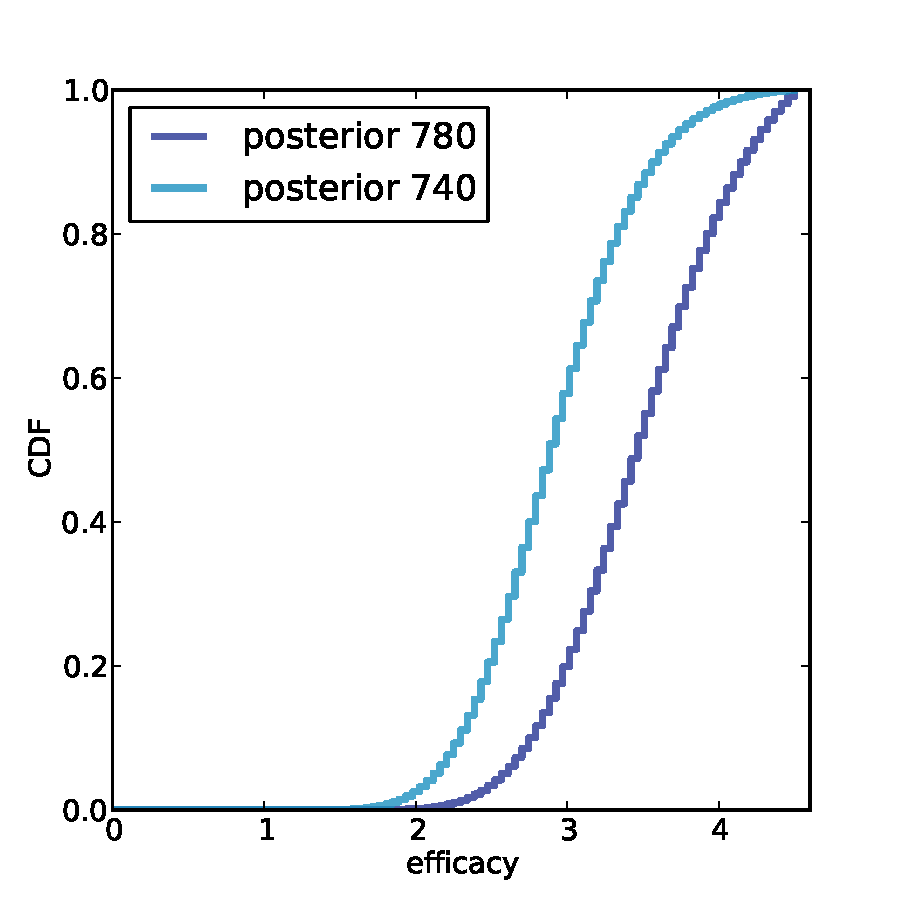
\includegraphics[height=2.5in]{figs/sat_posteriors_eff.pdf}}
\caption{Posterior distributions of efficacy for Alice and Bob.}
\label{fig.satposterior2}
\end{figure}

Now that the model is calibrated, we can compute the posterior
distribution of efficacy for Alice and Bob.  Here is a version of the
Sat class that works with the new model:

\begin{verbatim}
class Sat2(thinkbayes.Suite):

    def __init__(self, exam, score):
        thinkbayes.Suite.__init__(self)

        self.exam = exam
        self.score = score

        # start with the prior distribution
        efficacies = thinkbayes.MakeGaussianPmf(0, 1.5, 3)
        for efficacy, prob in efficacies.Items():
            self.Set(efficacy, prob)

        # update based on an exam score
        self.Update(score)
\end{verbatim}

The prior distribution of efficacy is
Gaussian with mean 0 and standard deviation 1.5 (and the suite of
hypotheses spans 3 standard deviations in each direction).

\verb"Sat2.Likelihood" computes the likelihood of a given test score
for a hypothetical level of efficacy.

\begin{verbatim}
    def Likelihood(self, hypo, data):
        efficacy = hypo
        score = data
        raw = self.exam.Reverse(score)

        pmf = self.exam.PmfCorrect(efficacy)
        like = pmf.Prob(raw)
        return like
\end{verbatim}

{\tt pmf} is the distribution of raw scores for a test-taker
with the given efficacy; {\tt like} is the probability of
the observed score.

Figure~\ref{fig.satposterior2} shows the posterior distributions
of efficacy for Alice and Bob.  As expected, the location
of Alice's distribution is farther to the right, but again there
is some overlap.

Using {\tt TopLevel} again, we compare $A$, the
hypothesis that Alice's efficacy is higher, and $B$, the
hypothesis that Bob's is higher.  The likelihood ratio is
3.4, a bit smaller than what we got from the simple model (3.8).
So this model indicates that the data are evidence in favor
of $A$, but a little weaker than the previous estimate.

If our prior belief is that $A$ and $B$ are equally likely,
then in light of this evidence we would give $A$ a posterior
probability of 77\%, leaving a 23\% chance that Bob's efficacy
is higher.


\section{Predictive distribution}

The analysis we have done so far generates estimates for
Alice and Bob's efficacy, but since efficacy is not directly
observable, it is hard to validate the results.

To give the model predictive power, we can use it to answer
another related question: ``If Alice and Bob take the math SAT
again, what is the chance that Alice will do better again?''

We'll answer this question in two steps:

\begin{itemize}

\item We'll use the posterior distribution of efficacy to
generate a predictive distribution of raw score for each test-taker.

\item We'll compare the two predictive distributions to compute
the probability that Alice gets a higher score again.

\end{itemize}

We already have most of the code we need.  To compute
the predictive distributions, we can use \verb"MakeRawScoreDist" again:

\begin{verbatim}
    exam = Exam()
    a_sat = Sat(exam, 780)
    b_sat = Sat(exam, 740)

    a_pred = exam.MakeRawScoreDist(a_sat)
    b_pred = exam.MakeRawScoreDist(b_sat)
\end{verbatim}

Then we can find the likelihood that Alice does better on the second
test, Bob does better, or they tie:

\begin{verbatim}
    a_like = thinkbayes.PmfProbGreater(a_pred, b_pred)
    b_like = thinkbayes.PmfProbLess(a_pred, b_pred)
    c_like = thinkbayes.PmfProbEqual(a_pred, b_pred)
\end{verbatim}

The probability that Alice does better on the second exam is 63\%,
which means that Bob has a 37\% chance of doing as well or better.

Notice that we have more confidence about Alice's efficacy than we do
about the outcome of the next test.  The posterior odds are 3:1 that
Alice's efficacy is higher, but only 2:1 that Alice will do better on
the next exam.


\section{Nuisance parameters}

\begin{figure}
% sat.py
\centerline{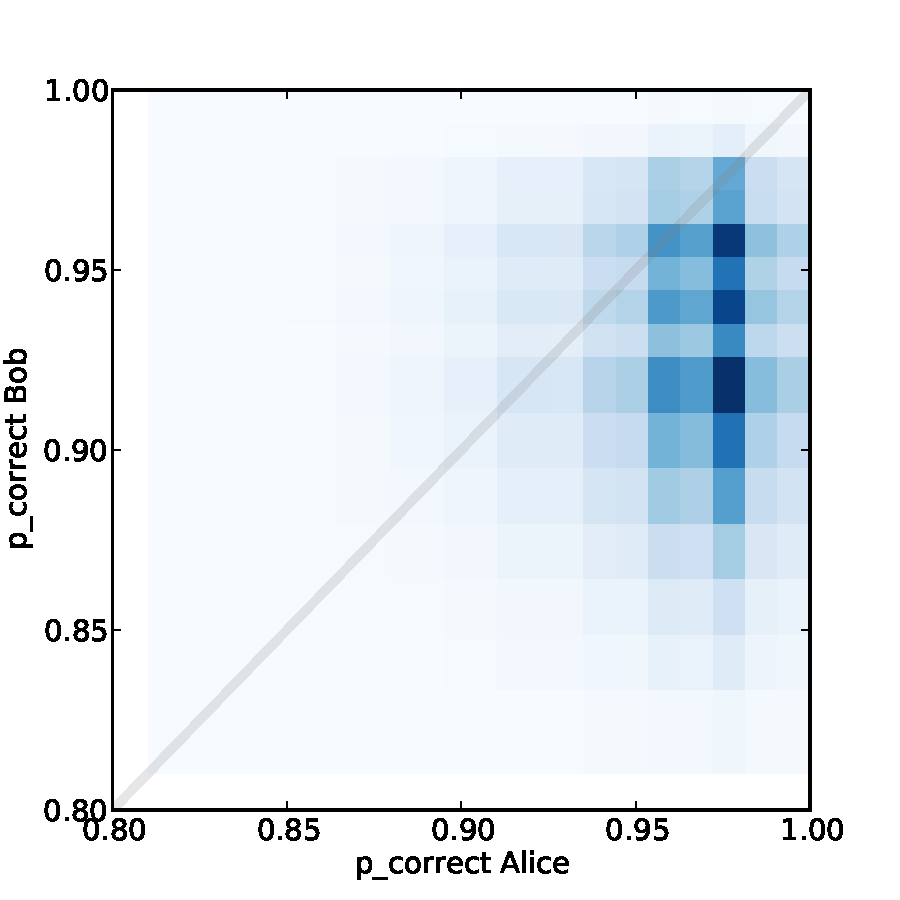
\includegraphics[height=2.5in]{figs/sat_joint.pdf}}
\caption{Joint posterior distribution of {\tt p\_correct} for Alice and Bob.}
\label{fig.satjoint}
\end{figure}

% TODO: make this figure equal aspect.

In this chapter we started with the question,
``How strong is the evidence that Alice is better prepared
than Bob?''  On the face of it, that sounds like we want to
test two hypotheses: either Alice is more prepared or Bob is.

But in order to compute likelihoods for these hypotheses, we
have to solve an estimation problem.  For each test-taker
we have to find the posterior distribution of either
\verb"p_correct" or \verb"efficacy".

We don't really care about these values, but we have
to estimate them to solve the problem we care about.  Which
is why values like this are called ``nuisance parameters.''

One way to visualize the analysis we did in this chapter is
to plot the space of these parameters.  \verb"thinkbayes.JointPmf"
takes two Pmfs, computes their joint distribution, and returns
a Pmf of each possible pair of values and its probability.

\begin{verbatim}
def JointPmf(pmf1, pmf2):
    pmf = Pmf()
    for v1, p1 in pmf1.Items():
        for v2, p2 in pmf2.Items():
            pmf.Set((v1, v2), p1 * p2)
    return pmf
\end{verbatim}

This function assumes that the two distributions are independent.

Figure~\ref{fig.satjoint} shows the joint posterior distribution of
\verb"p_correct" for Alice and Bob.  The diagonal like indicates the
part of the space where \verb"p_correct" is the same for Alice and
Bob.  To the right of this line, Alice is more prepared; to the left
Bob is more prepared.

In {\tt TopLevel.Update}, when we computed the likelihoods of $A$ and
$B$, we added up the probability mass each side of this line.  For the
cells that fall on the line, we added up the total mass and split it
between $A$ and $B$.

The process we used in this chapter---estimating a nuisance
variable in order to evaluate the likelihood of competing
hypotheses---is a common Bayesian approach to problems like this.




\chapter{Simulation}

In this chapter I describe my solution to a problem posed
by a patient with a kidney tumor.  I think the problem is interesting,
and important, because it is relevant to both the patient and
doctors treating other patients with these tumors.

And I think the solution is interesting because, although it
is a Bayesian approach to the problem, the use of Bayes's Theorem
is implicit.  I present the solution and my code; at the end
of the chapter I will explain the Bayesian part.

If you want more technical detail than I present here, you can
read my paper on this work at \url{http://arxiv.org/abs/1203.6890}.


\section{The Kidney Tumor problem}

I am a frequent reader and occasional contributor to the online statistics
forum at \url{http://reddit.com/r/statistics}.  In November 2011, I read
the following message:

\begin{quote}
"I have Stage IV Kidney Cancer and am trying to determine if the
  cancer formed before I retired from the military. ... Given the
  dates of retirement and detection is it possible to determine when
  there was a 50/50 chance that I developed the disease? Is it
  possible to determine the probability on the retirement date?  My
  tumor was 15.5 cm x 15 cm at detection. Grade II."
\end{quote}

I contacted the original poster and got more information; I learned
that veterans get different benefits if it is "more likely than not"
that a tumor formed while they were in military service (among other
considerations).

Because renal tumors grow slowly, and often do not cause symptoms,
they are sometimes left untreated.  As a result, doctors can observe
the rate of growth for untreated tumors by comparing scans from the
same patient at different times.  Several papers have reported these
growth rates.

I collected data from a paper by Zhang et al.\footnote{Zhang et al,
  Distribution of Renal Tumor Growth Rates Determined by Using Serial
  Volumetric CT Measurements, January 2009 {\it Radiology}, 250,
  137-144.}.  I contacted the authors to see if I could get raw data,
but they refused on grounds of medical privacy.  Nevertheless, I was
able to extract the data I needed by printing one of their graphs and
measuring it with a ruler.

\begin{figure}
% kidney.py
\centerline{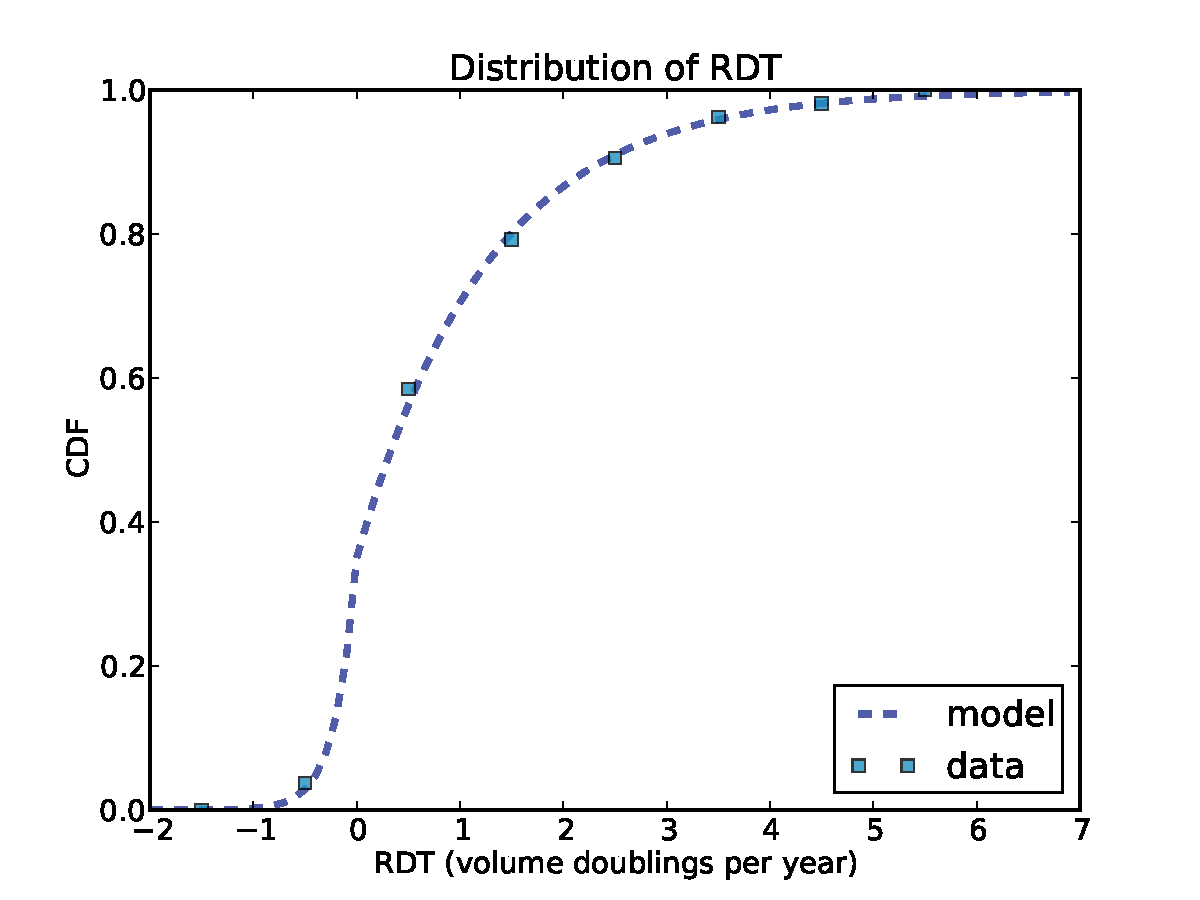
\includegraphics[height=2.5in]{figs/kidney2.pdf}}
\caption{CDF of RDT in doublings per year.}
\label{fig.kidney2}
\end{figure}

They report growth rates in reciprocal doubling time (RDT),
which is in units of doublings per year.  So a tumor with $RDT=1$
doubles in volume each year; with $RDT=2$ it quadruples in the same
time, and with $RDT=-1$, it halves.  Figure~\ref{fig.kidney2} shows the
distribution of RDT for 53 patients.

The squares are the data points from the paper; the line is a model I
fit to the data.  The positive tail fits an exponential distribution
well, so I used a mixture of two exponentials.


\section{A simple model}

It is usually a good idea to start with a simple model before
trying something more challenging.  Sometimes the simple model is
sufficient for the problem at hand, and if not, you can use it
to validate the more complex model.

For my simple model, I assume that tumors grow with a constant
doubling time, and that they are three-dimensional in the sense that
if the maximum linear measurement doubles, the volume is multiplied by
eight.

I learned from my correspondent that the time between his discharge
from the military and his diagnosis was 3291 days (about 9 years).
So my first calculation was, ``If this tumor grew at the median
rate, how big would it have been at the date of discharge?''

The median volume doubling time reported by Zhang et al.~is 811 days.
Assuming 3-dimensional geometry, the doubling time for a linear
measure is three times longer.

\begin{verbatim}
    # time between discharge and diagnosis, in days 
    interval = 3291.0

    # doubling time in linear measure is doubling time in volume * 3
    dt = 811.0 * 3

    # number of doublings since discharge
    doublings = interval / dt

    # how big was the tumor at time of discharge (diameter in cm)
    d1 = 15.5
    d0 = d1 / 2.0 ** doublings
\end{verbatim}

You can download the code in this chapter from
\url{http://thinkbayes.com/kidney.py}.  It depends on several other
modules in the same directory.  You can download them separately,
or check out the whole repository from \url{}.

The result, {\tt d0}, is about 6 cm.  So if this tumor formed after
the date of discharge, it must have grown substantially faster than
the median rate.  Therefore I concluded that it is ``more likely than
not'' that this tumor formed before the date of discharge.

In addition, I computed the growth rate that would be implied
if this tumor had formed after the date of discharge.  If we
assume an initial size of 0.1 cm, we can compute the number of
doublings to get to a final size of 15.5 cm:

\begin{verbatim}
    # assume an initial linear measure of 0.1 cm
    d0 = 0.1
    d1 = 15.5

    # how many doublings would it take to get from d0 to d1
    doublings = log2(d1 / d0)

    # what linear doubling time does that imply?
    dt = interval / doublings

    # compute the volumetric doubling time and RDT
    vdt = dt / 3
    rdt = 365 / vdt
\end{verbatim}

{\tt dt} is linear doubling time, so {\tt vdt} is volumetric
doubling time, and {\tt rdt} is reciprocal volumetric doubling
time.

The number of doublings, in linear measure, is 7.3, which implies
an RDT of 2.4.  In the data from Zhang et al, only 20\% of tumors
grew this fast during a period of observation.  So again,
I concluded that is ``more likely than not'' that the tumor
formed prior to the date of discharge.

These calculations are sufficient to answer the question as
posed, and on behalf of my correspondent, I wrote a letter explaining
my conclusions to the Veterans' Benefit Administration.

Later I told a friend, who is an oncologist, about my results.  He was
surprised by the growth rates observed by Zhang et al, and by what
they imply about the ages of these tumors.  He suggested that the
results might be interesting to researchers and doctors.

But in order to make them useful, I wanted a more general model
of the relationship between age and size.


\section{A more general model}

Given the size of a tumor at time of diagnosis, it would be most
useful to know the probability that the tumor formed before
any given date; in other words, the distribution of ages.

To find it, I run simulations of tumor growth to get the
distribution of size conditioned on age.  Then we can use
a Bayesian approach to get the
distribution of age conditioned on size.

The simulation starts with a small tumor and runs these steps:

\begin{itemize}

\item Choose a growth rate from the distribution of RDT.

\item Compute the size of the tumor at the end of an interval.

\item Record the size of the tumor at each interval

\item Repeat until the tumor exceeds the maximum relevant size.

\end{itemize}

For the initial size I chose 0.3 cm, because carcinomas smaller than
that are less likely to be invasive and less likely to have the blood
supply needed for rapid growth (see
\url{http://en.wikipedia.org/wiki/Carcinoma_in_situ}).  

I chose an interval of 245 days (about 8 months) because that is the
median time between measurements in the data source.

For the maximum size I chose 20 cm.  In the data source, the range of
observed sizes is 1.0 to 12.0 cm, so we are extrapolating beyond
the observed range at each end, but not by far, and not in a way
likely to have a strong effect on the results.

\begin{figure}
% kidney.py
\centerline{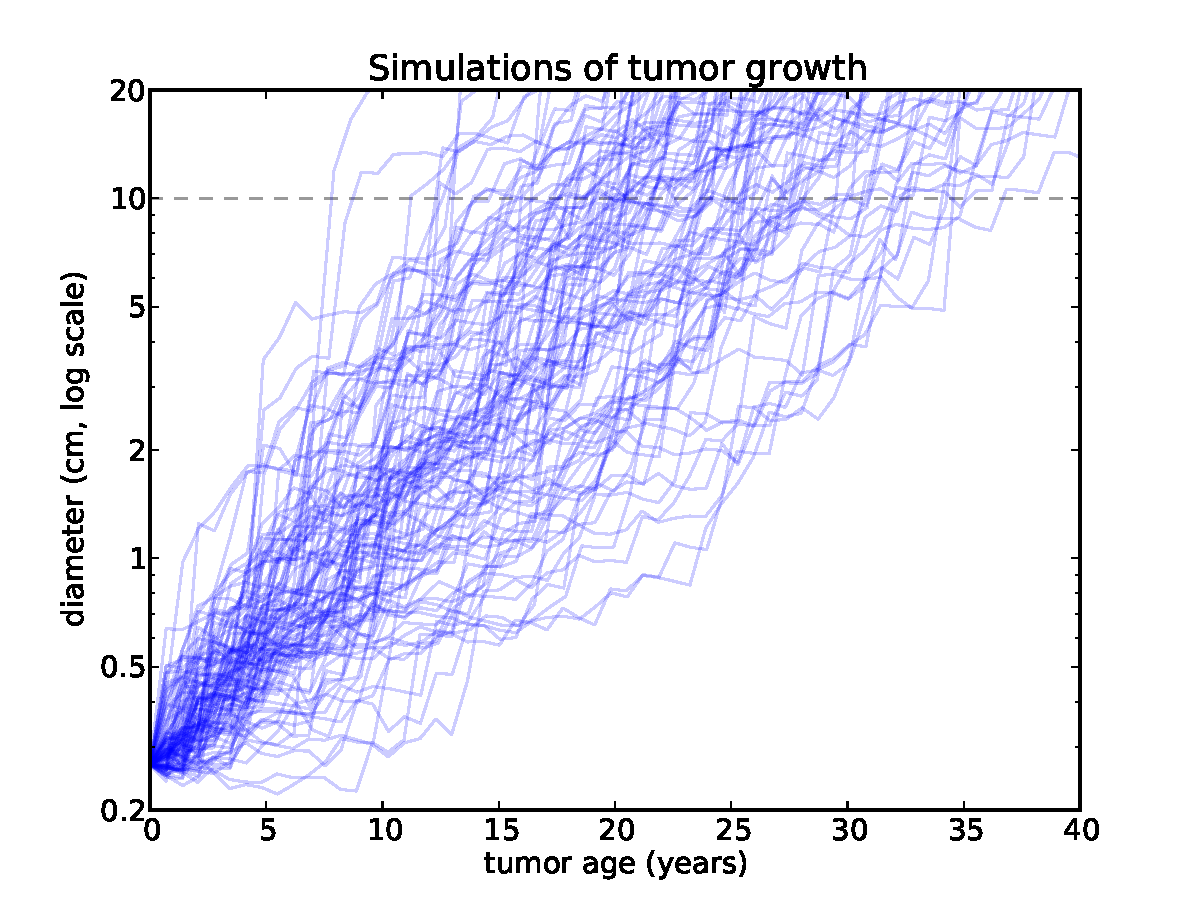
\includegraphics[height=2.5in]{figs/kidney4.pdf}}
\caption{Simulations of tumor growth, size vs. time.}
\label{fig.kidney4}
\end{figure}

The simulation is based on one big simplification:
the growth rate is chosen independently during each interval,
so it does not depend on age, size, or growth rate during
previous intervals.

In Section~\ref{serial} I will review these assumptions and
consider more detailed models.  But first let's look at some
examples.

Figure~\ref{fig.kidney4} shows 
the size of simulated tumors as a function of
age.  The dashed line at 10 cm shows the range of ages for tumors at
that size: the fastest-growing tumor gets there in 8 years; the
slowest takes more than 35.

I am presenting results in terms of linear measurements, but the
calculations are in terms of volume.  To convert from one to the
other, again, I use the volume of a sphere with the given
diameter.


\section{Implementation}

Here is the kernel of the simulation:

\begin{verbatim}
def MakeSequence(iterator, v0=0.01, interval=0.67, vmax=Volume(20.0)):
    seq = v0,
    age = 0

    for rdt in iterator:
        age += interval
        final, seq = ExtendSequence(age, seq, rdt, interval)
        if final > vmax:
            break

    return seq
\end{verbatim}

{\tt iterator} is an iterator object that yields a series of
random values from the CDF of growth rate.  {\tt MakeSequence}
takes the iterator as an argument so we can run it with
different random number generators, as you will see soon.

{\tt v0} is the initial volume in mL.  {\tt interval} is the time step
in years.  {\tt vmax} is the final volume corresponding to a linear
measurement of 20 cm.

{\tt Volume} converts from linear measurement in cm to volume
in mL, based on the simplification that the tumor is a sphere:

\begin{verbatim}
def Volume(diameter, factor=4*math.pi/3):
    return factor * (diameter/2.0)**3
\end{verbatim}

{\tt ExtendSequence} computes the volume of the tumor at the
end of the interval.

\begin{verbatim}
def ExtendSequence(age, seq, rdt, interval):
    initial = seq[-1]
    doublings = rdt * interval
    final = initial * 2**doublings
    new_seq = seq + (final,)
    cache.Add(age, new_seq, rdt)
    
    return final, new_seq
\end{verbatim}

{\tt age} is the age of the tumor at the end of the interval.
{\tt seq} is a tuple that contains the volumes so far.  {\tt rdt} is
the growth rate during the interval, in doublings per year.
{\tt interval} is the size of the time step in years.

The return values are {\tt final}, the volume of the
tumor at the end of the interval, and \verb"new_seq" a new
tuple containing the volumes in {\tt seq} plus the new volume
{\tt final}.

I am using a tuple so I can store it in the cache without
worrying about it being modified later.  The purpose of the
cache is to record the size and age of each tumor at the end
of each interval.


\section{Caching the joint distribution}

\begin{figure}
% kidney.py
\centerline{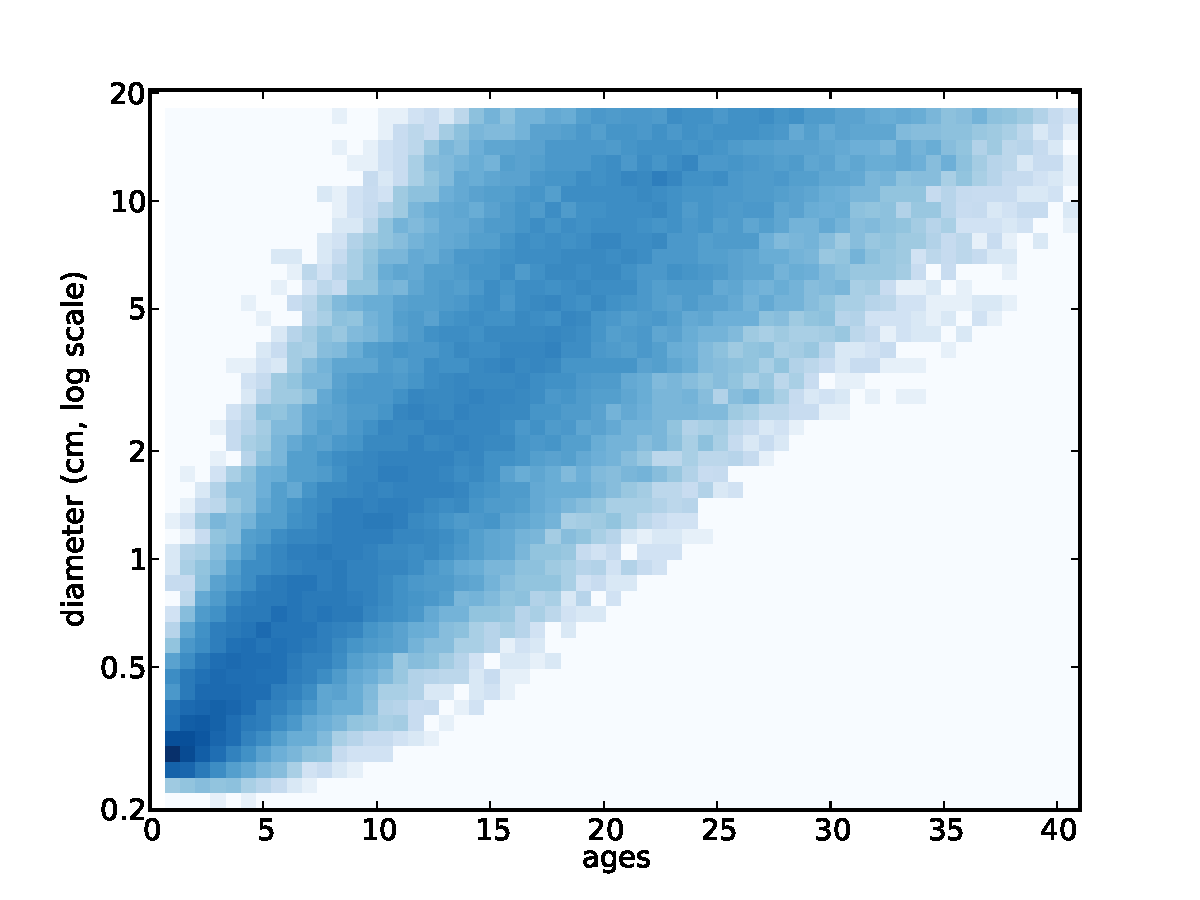
\includegraphics[height=2.5in]{figs/kidney8.pdf}}
\caption{Joint distribution of age and tumor size.}
\label{fig.kidney8}
\end{figure}


Here's how the cache works.  

\begin{verbatim}
class Cache(object):

    def __init__(self):
        self.joint = thinkbayes.Pmf()
\end{verbatim}

{\tt joint} is a Pmf that records 
frequency of each age-size pair, which approximates the
joint distribution of age and size.

At the end of each simulated interval, {\tt ExtendSequence} calls
{\tt Cache.Add}:

\begin{verbatim}
    def Add(self, age, seq):
        final = seq[-1]
        cm = Diameter(final)
        bucket = round(CmToBucket(cm))
        self.joint.Incr((age, bucket))
\end{verbatim}

Again, {\tt age} is the age of the tumor, and {\tt seq} is the
sequence of volumes so far.

Before adding the new data to the joint distribution, we use {\tt
  Diameter} to convert from volume to diameter in centimeters, and
{\tt CmToBucket} to convert from centimeters to a discrete bucket
number:

\begin{verbatim}
def CmToBucket(x, factor=10):
    return factor * math.log(x)
\end{verbatim}

The buckets are equally spaced on a log scale.  I chose the
factor 10 to yield a reasonable number of buckets.  For example,
1 cm maps to bucket 0; 10 cm maps to bucket 23.

After running the simulations, we can plot the joint distribution
as a pseudocolor plot, where each cell represents the number of
tumors observed at a given size-age pair.

Figure~\ref{fig.kidney8} shows the joint distribution after 1000
simulations.  As expected, the size of tumors typically increases
with age.

\section{Conditional distributions}

\begin{figure}
% kidney.py
\centerline{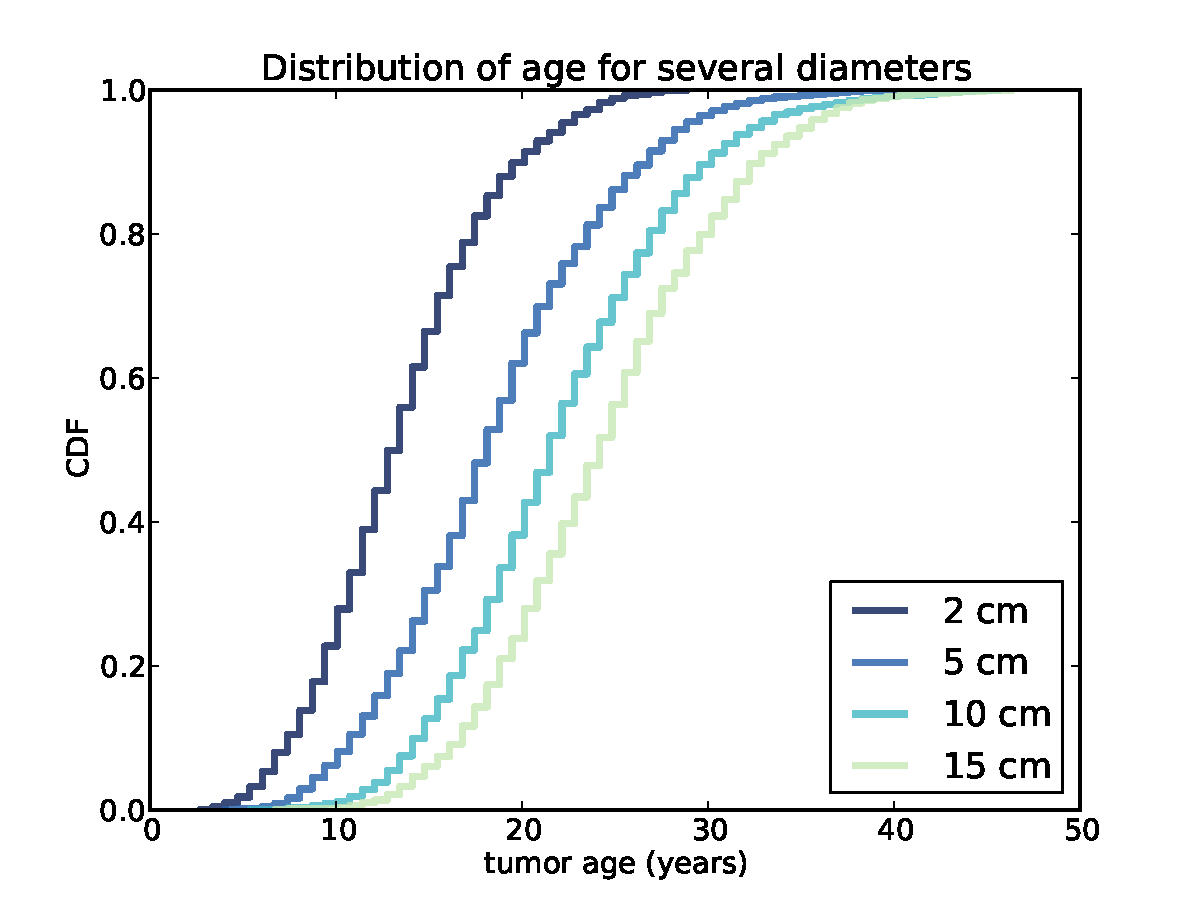
\includegraphics[height=2.5in]{figs/kidney6.pdf}}
\caption{Distributions of age, conditioned on size.}
\label{fig.kidney6}
\end{figure}

\begin{figure}
% kidney.py
\centerline{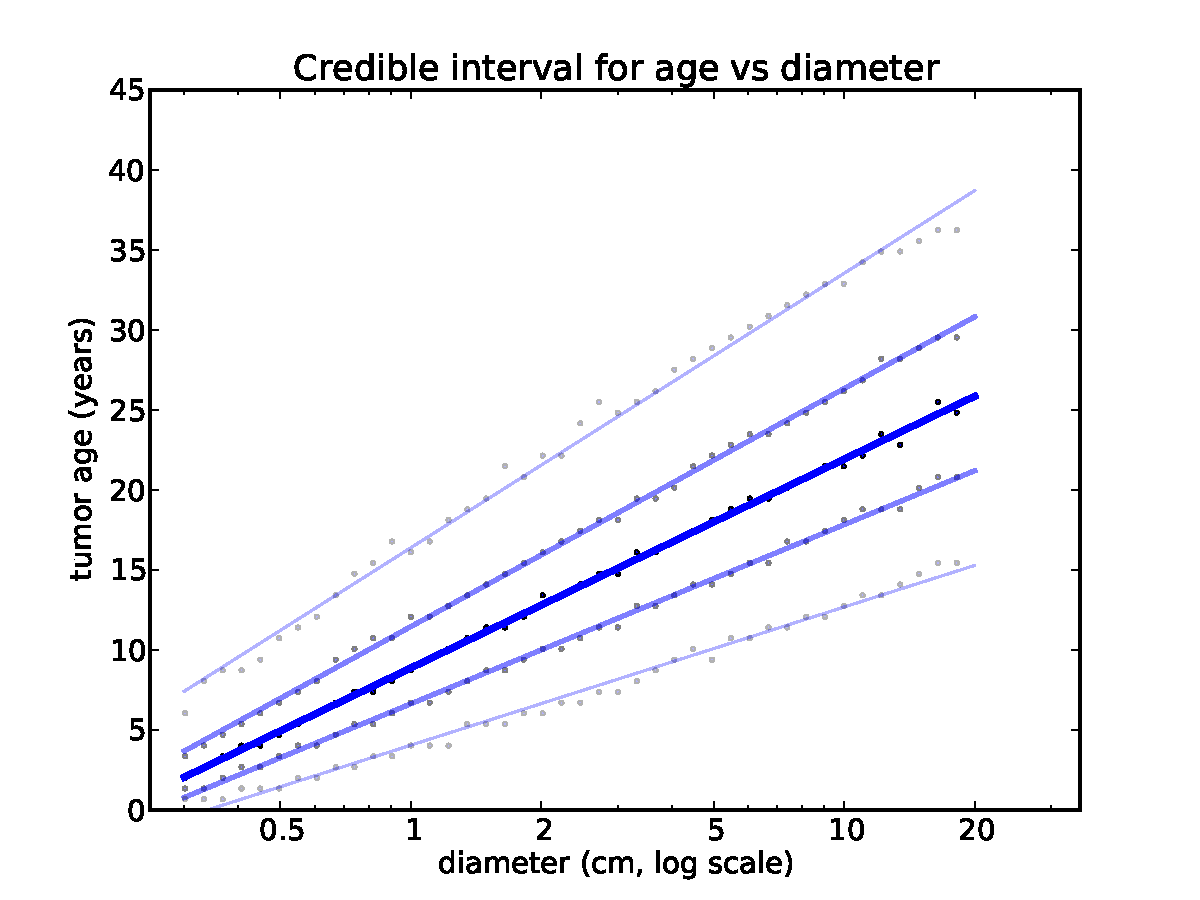
\includegraphics[height=2.5in]{figs/kidney7.pdf}}
\caption{Percentiles of tumor age as a function of size.}
\label{fig.kidney7}
\end{figure}

By taking a vertical slice from the joint distribution, we can get the
distribution of sizes for any given age.  By taking a horizontal
slice, we can get the distribution of ages conditioned on size.

% TODO: Rewrite this using the Joint distribution?

Here's the code that reads the joint distribution and builds
the conditional distribution for a given size bucket.

\begin{verbatim}
def ConditionalCdf(size_bucket):
    pmf = thinkbayes.Pmf()
    for val, prob in cache.GetItems():
        age, bucket = val
        if bucket == size_bucket:
            pmf.Set(age, prob)

    pmf.Normalize()
    cdf = thinkbayes.MakeCdfFromPmf(pmf)
    return cdf
\end{verbatim}

\verb"size_bucket" is the integer bucket number corresponding to a
particular size.  The return value is the CDF of age, conditioned
on the given size.

Figure~\ref{fig.kidney6} shows several of these CDFs, for
a range of sizes.  To summarize these distributions, we can
compute percentiles as a function of size.

\begin{verbatim}
    percentiles = [95, 75, 50, 25, 5]

    for bucket in cache.GetBuckets():
        cdf = ConditionalCdf(bucket)      
        ps = [cdf.Percentile(p) for p in percentiles]
\end{verbatim}

Figure~\ref{fig.kidney7} shows these percentiles for each
size bucket.  The data points are computed from the estimated
joint distribution.  There is some variability caused by making
time and size discrete, so I also show a least squares fit for
each sequence of percentiles.


\section{Serial Correlation}
\label{serial}

The results so far are based on a number of modeling decisions;
let's review them and consider which ones are the most
likely sources of error:

\begin{itemize}

\item To convert from linear measure to volume, we assume that
  tumors are approximately spherical.  This assumption is probably
  fine for tumors up to a few centimeters, but not for very
  large tumors.

\item The distribution of growth rates in the simulations are based on
  a continuous model we chose to fit the data reported by Zhang et al,
  which is based on 53 patients.  The fit is only approximate and, more
  importantly, a larger sample would yield a
  different distribution.

\item The growth model does not take into account tumor subtype or
  grade, which is consistent with the conclusion of Zhang et al:
  ``Growth rates in renal tumors of different sizes, subtypes and
  grades represent a wide range and overlap substantially.''
  But again, with a larger sample, difference might become apparent.

\item The distribution of growth rate does not depend on the size of
  the tumor.  This assumption is not realistic for very
  small and very large tumors, whose growth is limited by blood supply.

  But tumors observed by Zhang et al.~ranged from 1 to 12 cm, and they
  found no statistically significant relationship between
  size and growth rate.  So if there is a relationship, it is
  likely to be weak, at least in this size range.
  
\item In the simulations, growth rate during each interval is
  independent of previous growth rates.  It is plausible that, in
  reality, tumors that have grown quickly in the past are more likely
  to grow quickly.  In other words, there is probably
  a serial correlation in growth rate.

\end{itemize}

Of these, the first and last seem the most problematic.  I'll
investigate serial correlation first, then come back to
spherical geometry.

To simulate correlated growth, I wrote a generator\footnote{If you are
  not familiar with Python generators, see
  \url{http://wiki.python.org/moin/Generators}.} that yields a
correlated series from a given CDF.  Here's how the algorithm works:

\begin{enumerate}

\item Generate correlated values from a Gaussian distribution.
  This is easy to do because we can compute the distribution
  of the next value conditioned on the previous value.

\item Transform each value to its cumulative probability, using
  the Gaussian CDF.

\item Transform each cumulative probability to a value
  using the given CDF.

\end{enumerate}

Here's what that looks like in code:

\begin{verbatim}
def CorrelatedGenerator(cdf, rho):
    x = random.gauss(0, 1)
    yield Transform(x)

    sigma = math.sqrt(1 - rho**2);    
    while True:
        x = random.gauss(x * rho, sigma)
        yield Transform(x)
\end{verbatim}

{\tt cdf} is the desired CDF; {\tt rho} is the desired correlation.

The first value is Gaussian with mean 0 and standard deviation 1.

For subsequent values, the mean and standard deviation depend on the
previous value.  Given the previous $x$, the mean of the next value is
$\rho x$, and the variance is $1 - \rho^2$.

{\tt Transform} is the function that maps from
a Gaussian value to a value from the given CDF.

\begin{verbatim}
    def Transform(x):
        p = thinkbayes.GaussianCdf(x)
        y = cdf.Value(p)
        return y
\end{verbatim}

{\tt GaussianCdf} computes the CDF of the standard Gaussian
distribution at {\tt x}, returning a cumulative probability.
{\tt Cdf.Value} maps from a cumulative probability to the
corresponding value in {\tt cdf}.

Depending on the shape of {\tt cdf}, information can
be lost in transformation, so the actual correlation might be
lower than the target.  For example, when I generate
10000 values from the distribution of growth rates with
target correlation 0.4, the actual correlation is 0.37.
But since we are guessing at the right correlation anyway,
that's close enough.

Remember that {\tt MakeSequence} takes an iterator as an argument.
That interface allows it to work with different generators:

\begin{verbatim}
    iterator = UncorrelatedGenerator(cdf, rho)
    seq1 = MakeSequence(iterator)

    iterator = CorrelatedGenerator(cdf, rho)
    seq2 = MakeSequence(iterator)
\end{verbatim}

Now we can see what effect serial correlation has on the results;
the following table shows percentiles of age for a 6 cm tumor,
using the uncorrelated generator and a correlated generator
with target $\rho = 0.4$.

\begin{table}
\begin{tabular}{|l|r||r|r|r|r|r|}
\hline
Serial       & Diameter   & \multicolumn{5}{c|}{Percentiles of age} \\
Correlation  & (cm)       & 5th & 25th & 50th & 75th & 95th \\
\hline
0.0 & 6.0 & 10.7  & 15.4  & 19.5  & 23.5  & 30.2 \\
0.4 & 6.0 & 9.4  & 15.4  & 20.8  & 26.2  & 36.9 \\
\hline
\end{tabular}

\caption{Percentiles of tumor age conditioned on size.}
\end{table}

Correlation makes the fastest growing tumors faster and the slowest
slower, so the range of ages is wider.  The difference is modest for
low percentiles, but for the 95th percentile it is more than 6 years.
To compute these percentiles precisely, we would need a better
estimate of the actual serial correlation.

However, this model is sufficient to answer the question
we started with: given a tumor with a linear dimension of
15.5 cm, what is the probability that it formed more than
8 years ago?

Here's the code:

\begin{verbatim}
def ProbOlder(cm, age):
    bucket = CmToBucket(cm)
    cdf = ConditionalCdf(bucket)
    p = cdf.Prob(age)
    return 1-p
\end{verbatim}

{\tt cm} is the size of the tumor; {\tt age} is the age threshold
in years.  With no serial correlation, the probability that a
15.5 cm tumor is older than 8 years is 0.999, or almost certain.
With correlation 0.4, faster-growing tumors are more likely, but
the probability is still 0.995.  Even with correlation 0.8, the
probability is 0.978.

Another likely source of error is the assumption that tumors are
approximately spherical.  For a tumor with linear dimensions 15.5 x 15
cm, this assumption is probably not valid.  If, as seems likely, it
were relatively flat, it might have the same volume as a 6 cm sphere.
But with this smaller volume and correlation 0.8, the probability of age
greater than 8 is still 95\%.

So even taking into account modeling errors, it is unlikely that such
a large tumor could have formed less than 8 years prior to the date of
diagnosis.


\section{Where's Bayes?}

Well, we got through a whole chapter without using Bayes's Theorem or
the {\tt Suite} class that encapsulates Bayesian updates.  What
happened?

One way to think about Bayes's Theorem is as an algorithm for
inverting conditional probabilities.  Given \p{B|A}, we can compute
\p{A|B}, provided we know \p{A} and \p{B}.  Of course this algorithm
is only useful if, for some reason, it is easier to compute \p{B|A}
than \p{A|B}.

In this example, it is.  By running simulations, we can estimate the
distribution of size conditioned on age, or \p{size|age}.  But it is
harder to get the distribution of age conditioned on size, or
\p{age|size}.  So this seems like a perfect opportunity to use Bayes's
Theorem.

The reason I didn't is computational efficiency.  To estimate
\p{size|age} for any given size, you have to run a lot of simulations.
Along the way, you end up computing \p{size|age} for a lot of sizes.
In fact, you end up computing the entire joint distribution of size
and age, \p{size, age}.

And once you have the joint distribution, you don't really need
Bayes's Theorem, you can extract \p{age|size} by taking slices from
the joint distribution, as demonstrated in {\tt ConditionalCdf}.

So we side-stepped Bayes, but he was with us in spirit.


\chapter{A hierarchical model}
\label{species}

\section{Belly button bacteria}

Belly Button Biodiversity 2.0 (BBB2) is a nation-wide citizen
science project with the goal of identifying bacterial species that
can be found in human navels (\url{http://bbdata.yourwildlife.org}).
The project might seem whimsical, but it is part of an increasing
interest in the human microbiome, the set of microorganisms that live
on human skin and other surfaces that contact the environment.

In their pilot study, BBB2 researchers collected swabs from the navels
of 60 volunteers, used multiplex pyrosequencing to extract and sequence
fragments of 16S rDNA, then identified the species or genus the
fragments came from.  Each identified fragment is called a ``read.''

We can use these data to answer several related questions:

\begin{itemize}

\item Based on the number of species observed, can we estimate
  the total number of species in the environment?

\item Can we estimate the prevalence of each species; that is, the
  fraction of the total population belonging to each species?

\item If we are planning to collect additional samples, can we predict
  how many new species we are likely to discover?

\item How many additional reads are needed to increase the
  fraction of observed species to a given threshold?

\end{itemize}

These questions make up what is called the ``unseen species problem.''


\section{Lions and tigers and bears}

I'll start with a simplified version of the problem where we know that
there are exactly three species.  Let's call them lions, tigers and
bears.  Suppose we visit a wild animal preserve and see 3 lions, 2
tigers and one bear.

If we have an equal chance of observing any animal in the preserve
then the number of each species we see is governed by the multinomial
distribution.  If the prevalence of lions and tigers and bears is
\verb"p_lion" and \verb"p_tiger" and \verb"p_bear", the likelihood of
seeing 3 lions, 2 tigers and one bear is

\begin{verbatim}
p_lion**3 * p_tiger**2 * p_bear**1
\end{verbatim}

An approach that is tempting, but not correct, is to use beta
distributions, as in Section~\ref{beta}, to describe the prevalence of
each species separately.  For example, we saw 3 lions and 3 non-lions;
if we think of that as 3 ``heads'' and 3 ``tails,'' then the posterior
distribution of \verb"p_lion" is:

\begin{verbatim}
    beta = thinkbayes.Beta()
    beta.Update((3, 3))
    print beta.MaximumLikelihood()
\end{verbatim}

The maximum likelihood estimate for \verb"p_lion" is the observed
rate, 50\%.  Similarly the MLEs for \verb"p_tiger" and \verb"p_bear"
are 33\% and 17\%.

But there are two problems:

\begin{itemize}

\item We have implicitly used a prior for each species that is uniform
  from 0 to 1, but since we know that there are three species, that
  prior is not correct.  The right prior should have a mean of 1/3,
  and there should be zero likelihood that any species has a
  prevalence of 100\%.

\item The distributions for each species are not independent, because
  the prevalences have to add up to 1.  To capture this dependence, we
  need a joint distribution for the three prevalences.

\end{itemize}

We can use a Dirichlet distribution to solve both of these problems
(see \url{http://en.wikipedia.org/wiki/Dirichlet_distribution}).  In
the same way we used the beta distribution to describe the
distribution of bias for a coin, we can use a Dirichlet
distribution to describe the joint distribution of \verb"p_lion",
\verb"p_tiger" and \verb"p_bear".

The Dirichlet distribution is the multi-dimensional generalization
of the beta distribution.  Instead of two possible outcomes, like
heads and tails, the Dirichlet distribution handles any number of
outcomes: in this example, three species.

If there are {\tt n} outcomes, the Dirichlet distribution is
described by {\tt n} parameters, written $\alpha_1$ through $\alpha_n$.

Here's the definition, from {\tt thinkbayes.py}, of a class that
represents a Dirichlet distribution:

\begin{verbatim}
class Dirichlet(object):

    def __init__(self, n):
        self.n = n
        self.params = numpy.ones(n, dtype=numpy.int)
\end{verbatim}

{\tt n} is the number of dimensions; initially the parameters
are all 1.  I use a {\tt numpy} array to store the parameters
so I can take advantage of array operations.

Given a Dirichlet distribution, the marginal distribution
for each prevalence is a beta distribution, which we can
compute like this:

\begin{verbatim}
    def MarginalBeta(self, i):
        alpha0 = self.params.sum()
        alpha = self.params[i]
        return Beta(alpha, alpha0-alpha)
\end{verbatim}

{\tt i} is the index of the marginal distribution we want.
{\tt alpha0} is the sum of the parameters; {\tt alpha} is the
parameter for the given species.

In the example, the prior marginal distribution for each species
is {\tt Beta(1, 2)}.  We can compute the prior means like
this:

\begin{verbatim}
    dirichlet = thinkbayes.Dirichlet(3)
    for i in range(3):
        beta = dirichlet.MarginalBeta(i)
        print beta.Mean()
\end{verbatim}

As expected, the prior mean prevalence for each species is 1/3.

To update the Dirichlet distribution, we add the number of
observations to each parameter, like this:

\begin{verbatim}
    def Update(self, data):
        m = len(data)
        self.params[:m] += data
\end{verbatim}

Here {\tt data} is a sequence of counts in the same order as {\tt
  params}, so in this example, it should be the number of lions,
tigers and bears.

But {\tt data} can be shorter than {\tt params}; in that
case there are some hypothetical species that have not been
observed.

Here's code that updates {\tt dirichlet} with the observed data and
computes the posterior marginal distributions.

\begin{verbatim}
    data = [3, 2, 1]
    dirichlet.Update(data)

    for i in range(3):
        beta = dirichlet.MarginalBeta(i)
        pmf = beta.MakePmf()
        print i, pmf.Mean()
\end{verbatim}

\begin{figure}
% species.py
\centerline{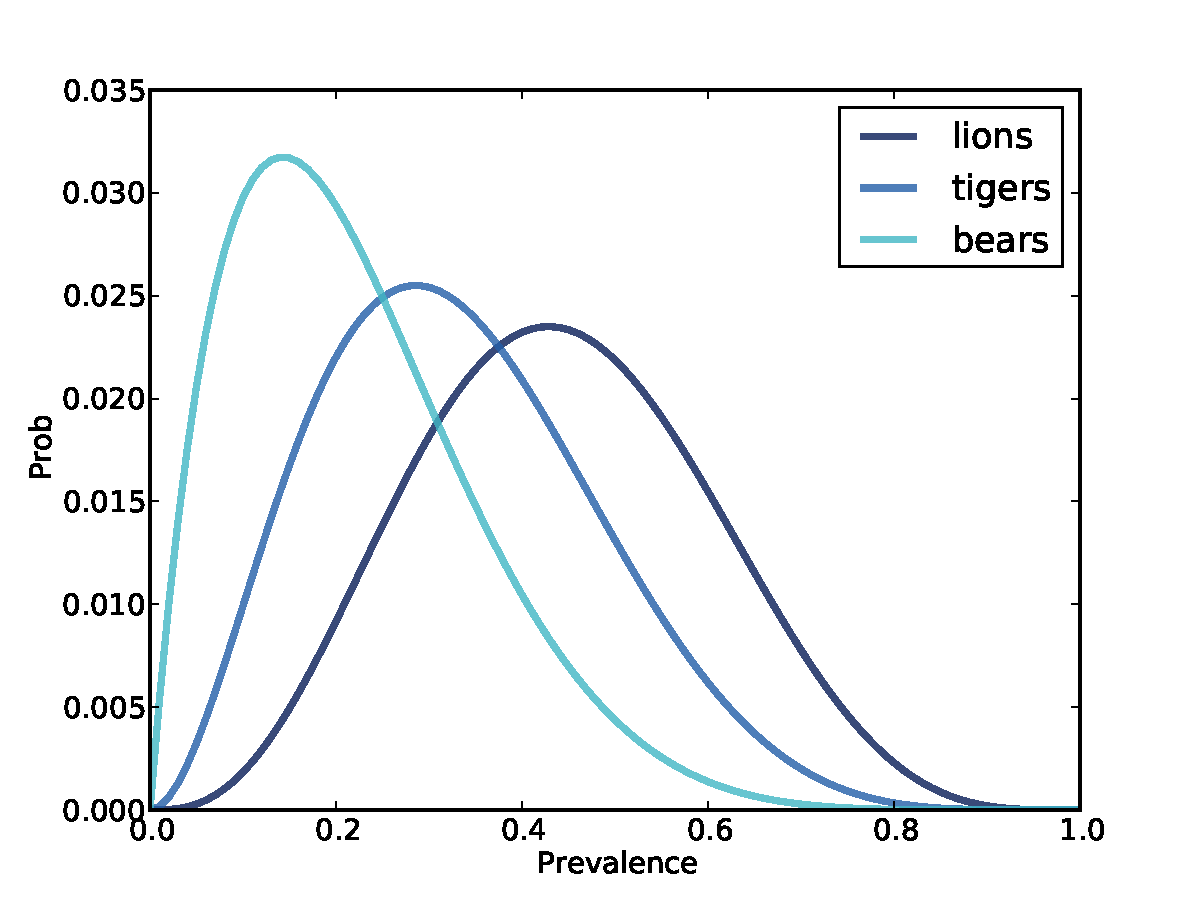
\includegraphics[height=2.5in]{figs/species1.pdf}}
\caption{Distribution of prevalences for three species.}
\label{fig.species1}
\end{figure}

Figure~\ref{fig.species1} shows the results.  The posterior
mean prevalences are 44\%, 33\% and 22\%.


\section{A hierarchical model}

We have solved a simplified version of the problem: if we
know how many species there are, we can estimate the prevalence
of each.

Now let's get back to the original problem, estimating the total
number of species.  To solve this problem I'll define a metasuite,
which is a Suite that contains other Suites as hypotheses.  In this
case, the top-level Suite contains hypotheses about the number of
species; the bottom level contains hypotheses about prevalences.
A multi-level model like this is called ``hierarchical.''

Here's the class definition:

\begin{verbatim}
class Species(thinkbayes.Suite):

    def __init__(self, ns):
        hypos = [thinkbayes.Dirichlet(n) for n in ns]
        thinkbayes.Suite.__init__(self, hypos)
\end{verbatim}

\verb"__init__" takes a list of possible values for {\tt n} and
makes a list of Dirichlet objects.

Here's the code that creates the top-level suite:

\begin{verbatim}
    ns = range(3, 30)
    suite = Species(ns)
\end{verbatim}

{\tt ns} is the list of possible values for {\tt n}.  We have seen 3
species, so there have to be at least that many.  I chose an upper
bound that seemed reasonable, but we will have to check later that the
probability of exceeding this bound is low.  And at least initially
we assume that any value in this range is equally likely.

To update a hierarchical model, you have to update all levels.
Sometimes it is necessary or more efficient to update the bottom
level first and work up.  In this case it doesn't matter, so
I update the top level first:

\begin{verbatim}
#class Species

    def Update(self, data):
        thinkbayes.Suite.Update(self, data)
        for hypo in self.Values():
            hypo.Update(data)
\end{verbatim}

{\tt Species.Update} invokes {\tt Update} in the parent class,
then loops through the sub-hypotheses and updates them.

Now all we need is a likelihood function.  As usual,
{\tt Likelihood} gets a hypothesis and a dataset as arguments:

\begin{verbatim}
# class Species

    def Likelihood(self, hypo, data):
        dirichlet = hypo
        like = 0
        for i in range(1000):
            like += dirichlet.Likelihood(data)

        return like
\end{verbatim}

{\tt hypo} is a Dirichlet object; {\tt data} is a sequence of
observed counts.  {\tt Species.Likelihood} calls
{\tt Dirichlet.Likelihood} 1000 times and returns the total.

Why do we have to call it 1000 times?  Because {\tt
  Dirichlet.Likelihood} doesn't actually compute the likelihood of the
data under the whole Dirichlet distribution.  Instead, it draws one
sample from the hypothetical distribution and computes the likelihood
of the data under the sampled set of prevalences.

Here's what it looks like:

\begin{verbatim}
# class Dirichlet

    def Likelihood(self, data):
        m = len(data)
        if self.n < m:
            return 0

        x = data
        p = self.Random()
        q = p[:m]**x
        return q.prod()
\end{verbatim}

The length of {\tt data} is the number of species observed.  If
we see more species than we thought existed, the likelihood is 0.

Otherwise we select a random set of prevalences, {\tt p}, and
compute the multinomial PDF, which is
%
\[ c(x) \prod_i p_i^{x_i}\]
%
$p_i$ is the prevalence of the $i$th species, and $x_i$ is the
observed number.  The first term, $c(x)$, is the multinomial
coefficient; I left it out of the computation because it is
a multiplicative factor that depends only
on the data, not the hypothesis, so it gets normalized away
(see \url{http://en.wikipedia.org/wiki/Multinomial_distribution}).

Also, I truncated {\tt p} at {\tt m}, which is the number of
observed species.  For the unseen species, $x_i$ is 0, so
$p_i^{x_i}$ is 1, so we can leave them out of the product.


\section{Random sampling}

There are two ways to generate a random sample from a Dirichlet
distribution.  One is to use the marginal beta distributions, but in
that case you have to select one at a time and scale the rest so they
add up to 1 (see
\url{http://en.wikipedia.org/wiki/Dirichlet_distribution#Random_number_generation}).

A less obvious, but faster, way is to select values from {\tt n} gamma
distributions, then normalize by dividing through by the total. 
Here's the code:

\begin{verbatim}
# class Dirichlet

    def Random(self):
        p = numpy.random.gamma(self.params)
        return p / p.sum()
\end{verbatim}

Now we're ready to look at some results.  Here is the code that
updates the top-level suite and extracts the posterior PMF of {\tt n}:

\begin{verbatim}
    data = [3, 2, 1]
    suite.Update(data)
    pmf = suite.DistOfN()
\end{verbatim}

To get the posterior distribution of {\tt n}, {\tt DistOfN} iterates
through the top-level hypotheses:

\begin{verbatim}
    def DistOfN(self):
        pmf = thinkbayes.Pmf()
        for hypo, prob in self.Items():
            pmf.Set(hypo.n, prob)
        return pmf
\end{verbatim}

\begin{figure}
% species.py
\centerline{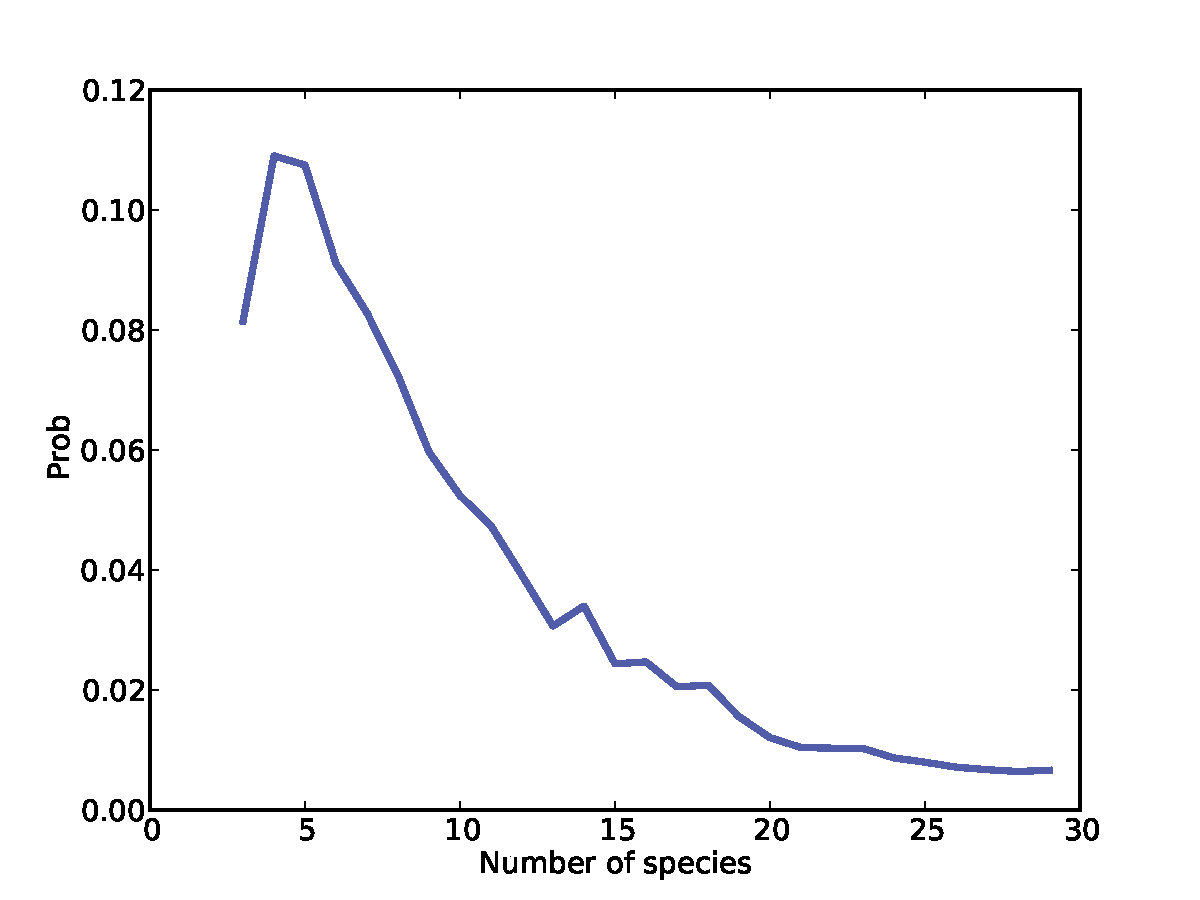
\includegraphics[height=2.5in]{figs/species2.pdf}}
\caption{Distribution of prevalences for three species.}
\label{fig.species2}
\end{figure}

Figure~\ref{fig.species2} shows the result.  The most likely value is 4.
Values from 3 to 8 are all likely; after that the probabilities
drop off quickly.  The probability that there are 29 species is
low enough to be negligible; if we chose a higher bound, 
we would get the same result.

But remember that we started with a uniform prior for {\tt n}.  If we
have background information about the number of species in the
environment, we might choose a different prior.


\section{Optimization}

I have to admit that I am proud of this example.  The unseen species
problem is not easy, and I think this solution is simple and clear,
and takes surprisingly few lines of code (about 50 so far).

The only problem is that it is slow.  It's good enough for the example
with only 3 observed species, but not good enough for the belly button
data, with more than 100 species in some samples.

The next few sections present a series of optimizations we need to
make this solution scale.  Before we get into the details, here's
a road map.

\begin{itemize}

\item The first step is to recognize that if we update the Dirichlet
  distributions with the same data, the first {\tt m} parameters are
  the same for all of them.  The only difference is the number of
  hypothetical unseen species.  So we don't really need {\tt n}
  Dirichlet objects; we can store the parameters in the top level of
  the hierarchy.  {\tt Species2} implements this optimization.

\item {\tt Species2} also uses the same set of random values for all
  of the hypotheses.  This saves time generating random values, but it
  has a second benefit that turns out to be more important: by giving
  all hypothesis the same selection from the sample space, we make
  the comparison between the hypotheses more fair, so it takes
  fewer iterations to converge.

\item But there is still a major performance problem.  As the
  number of observed species increases, the array of random
  prevalences gets bigger, and the chance of choosing one that is
  approximately right becomes small.  So the vast majority
  of iterations yield small likelihoods that don't contribute
  much to the total, and don't discriminate between hypotheses.

  The solution is to do the updates one species at a time.  {\tt
  Species4} is a simple implementation of this strategy using
  Dirichlet objects to represent the sub-hypotheses.

\item Finally, {\tt Species5} combines the sub-hypothesis into the top
  level and uses {\tt numpy} array operations to speed things up.

\end{itemize}

If you are not interested in the details, feel free to skip to
Section~\ref{belly} where we look at some results from the belly
button data.


\section{Collapsing the hierarchy}
\label{collapsing}

As I said, all of the bottom-level Dirichlet distributions are updated
with the same data, so the first {\tt m} parameters are the same for
all of them.

Since the bottom-level Dirichlet distributions all contain the same
information, we can eliminate them and merge the parameters into
the top-level suite.  {\tt Species2} implements this optimization:

\begin{verbatim}
class Species2(object):
    
    def __init__(self, ns):
        self.ns = ns
        self.probs = numpy.ones(len(ns), dtype=numpy.double)
        self.params = numpy.ones(self.high, dtype=numpy.int)
\end{verbatim}

{\tt ns} is the list of hypothetical values for {\tt n};
{\tt probs} is the list of corresponding probabilities.  And
{\tt params} is the sequence of Dirichlet parameters, initially
all 1.

Here's the {\tt Update} function that updates both levels of
the hierarchy: first the probability for each value of {\tt n},
then the Dirichlet parameters:

\begin{verbatim}
# class Species2

    def Update(self, data):
        like = numpy.zeros(len(self.ns), dtype=numpy.double)
        for i in range(1000):
            like += self.SampleLikelihood(data)

        self.probs *= like
        self.probs /= self.probs.sum()

        m = len(data)
        self.params[:m] += data
\end{verbatim}

{\tt SampleLikelihood} returns an array of likelihoods, one for
each value of {\tt n}.  {\tt like} accumulates the total likelihood
for 1000 samples.  {\tt self.probs}
is multiplied by the total likelihood, then normalized.
Finally, updating the parameters is identical to what we saw in {\tt
  Dirichlet.Update}.

Now let's look at {\tt SampleLikelihood}.  There are two
opportunities for optimization here:

\begin{itemize}

\item When the hypothetical number of species, {\tt n},
exceeds the observed number, {\tt m}, we only need the first {\tt m}
terms of the multinomial PDF; the rest are 1.

\item If the number of species is large, the likelihood of the data
might be too small for floating-point.  So it is safer to compute
log-likelihoods.  For the multinomial PDF, it is also faster.

\end{itemize}

Again, the multinomial PDF is
%
\[ c(x) \prod_i p_i^{x_i}\]
%
So the log-likelihood is
%
\[ log(c(x)) + \sum_i \log(p_i) * x_i \]
%
which is fast and easy to compute.  Here's the code:

\begin{verbatim}
# class Species2

    def SampleLikelihood(self, data):
        gammas = numpy.random.gamma(self.params)

        m = len(data)
        row = gammas[:m]
        col = numpy.cumsum(gammas)

        log_likes = []
        for n in self.ns:
            ps = row / col[n-1]
            terms = numpy.log(ps) * data
            log_like = terms.sum()
            log_likes.append(log_like)

        log_likes -= numpy.max(log_likes)
        likes = numpy.exp(log_likes)

        coefs = [thinkbayes.BinomialCoef(n, m) for n in self.ns]
        likes *= coefs

        return likes
\end{verbatim}

{\tt gammas} is an array of values from a gamma distribution; its
length is the largest hypothetical value of {\tt n}.  {\tt row} is
just the first {\tt m} elements of {\tt gammas}; since these are the
only elements that depend on the data, they are the only ones we need.

For each value of {\tt n} we need to divide {\tt row} by the
total of the first {\tt n} values from {\tt gamma}.  {\tt cumsum}
computes these cumulative sums and stores them in {\tt col}.

The loop iterates through the values of {\tt n} and accumulates
a list of log-likelihoods.

Inside the loop, {\tt ps} contains the row of probabilities, normalized
with the appropriate cumulative sum.  {\tt terms} contains the
terms of the summation, $\log(p_i) x_i$, and \verb"log_like" contains
their sum.

After the loop, we want to convert the log-likelihoods to linear
likelihoods, but first it's a good idea to shift them so the largest
log-likelihood is 0; that way the linear likelihoods are not too
small.

Finally, before we return the likelihood, we have to apply a correction
factor, which is the number of ways we could have observed these {\tt m}
species, if the total number of species is {\tt n}.  The binomial
coefficient is the fancy name for ``n choose m'', which is written
$\binom{n}{m}$. 

As often happens, the optimized version is less readable and more
error-prone than the original.  But that's one reason I think it is
a good idea to start with the simple version; we can use it for
regression testing.  I plotted results from both versions and confirmed
that they are approximately equal, and that they converge as the
sample size increases.


\section{One more problem}

There's more we could do to optimize this version, but there's a 
problem we need to work on first.  As the number of observed
species increases, this version gets noisier and takes more
iterations to converge on a good answer.

The problem is that if the probabilities we choose from the Dirichlet
distribution, the {\tt ps}, are not at least approximately right,
the likelihood of the observed data is close to zero and almost
equally bad for all values of {\tt n}.  So most iterations don't
provide any useful contribution to the total likelihood.  And as the
number of observed species, {\tt m}, gets large, the probability of
choosing {\tt ps} with non-negligible likelihood gets small.  Really
small.

Fortunately, there is a solution.  Remember that if you observe
a set of data, you can update the prior distribution with the
entire dataset, or you can break it up into a series of updates
with subsets of the data, and the result is the same either way.

For this example, the key is to perform the updates one species at
a time.  That way when we generate a random set of {\tt ps}, only
one of them affects the computed likelihood, so the chance of choosing
a good one is much better.

Here's a new version that updates one species at a time:

\begin{verbatim}
class Species4(Species):

    def Update(self, data):
        m = len(data)

        for i in range(m):
            one = numpy.zeros(i+1)
            one[i] = data[i]            
            Species.Update(self, one)
\end{verbatim}

This version inherits \verb"__init__" from {\tt Species}, so it
represents the hypotheses as a list of Dirichlet objects (unlike
{\tt Species2}).

{\tt Update} loops through the observed species and makes an
array, {\tt one}, with all zeros and one species count.  Then
is calls {\tt Update} in the parent class, which actually computes
the likelihoods and updates the sub-hypotheses.

So in the running example, we do three updates.  The first
is something like ``I have seen three lions.''  The second is
``I have see two tigers and no additional lions.''  And the third
is ``I have seen one bear and no more lions and tigers.''

So here's the new version of {\tt Likelihood}:

\begin{verbatim}
# class Species4

    def Likelihood(self, hypo, data):
        dirichlet = hypo
        like = 0
        for i in range(self.iterations):
            like += dirichlet.Likelihood(data)

        # correct for the number of unseen species the new one
        # could have been
        m = len(data)
        num_unseen = dirichlet.n - m + 1
        like *= num_unseen

        return like
\end{verbatim}

This is almost the same as {\tt Species.Likelihood}.  The difference
is the factor, \verb"num_unseen".  This correction is necessary
because each time we see a species for the first time, we have to
consider that there were some number of other unseen species that
we might have seen.  For larger values of {\tt n} there are more
unseen species that we could have seen, which increases the likelihood
of the data.

This is a subtle point and I have to admit that I did not get it right
the first time.  But again I was able to validate this version
by comparing it to the previous versions.


\section{We're not done yet}

\newcommand{\BigO}[1]{\mathcal{O}(#1)}

Performing the updates one species at a time solves one problem, but
it creates another.  Each update takes time proportional to $n m$,
so if we do $m$ updates, the algorithm is $\BigO{n m^2}$. 

But we can speed things up using the same trick we used in
Section~\ref{collapsing}: we'll get rid of the Dirichlet objects and
collapse the two levels of the hierarchy into a single object.  So
here's yet another version of {\tt Species}:

\begin{verbatim}
class Species5(Species2):
    
    def Update(self, data):
        m = len(data)
        for i in range(m):
            self.UpdateOne(i+1, data[i])
            self.params[i] += data[i]
\end{verbatim}

This version inherits \verb"__init__" from {\tt Species2}, so
it uses {\tt ns} and {\tt probs} to represent the distribution
of {\tt n}, and {\tt params} to represent the parameters of
the Dirichlet distribution.

{\tt Update} is similar to what we saw in the previous section.
It loops through the observed species and calls {\tt UpdateOne}.
One difference is that {\tt UpdateOne} doesn't get the whole list
of species counts; it just gets the index (which species was
observed) and the count (how many of them there were).

Now here's {\tt UpdateOne}:

\begin{verbatim}
# class Species5

    def UpdateOne(self, m, count):
        likes = numpy.zeros(len(self.ns), dtype=numpy.double)
        for i in range(self.iterations):
            likes += self.SampleLikelihood(m, count)

        unseen_species = [n-m+1 for n in self.ns]
        likes *= unseen_species

        self.probs *= likes
        self.probs /= self.probs.sum()
\end{verbatim}

This function is similar to {\tt Species2.Update}, with two changes:

\begin{itemize}

\item The interface is different.  Instead of the whole dataset,
we get {\tt m}, the number
of species we have seen, and {\tt count}, how many of that
species we've seen.

\item We have to apply a correction factor for the number
of unseen species, as in {\tt Species4.Likelihood}.  The difference
here is that we update all of the likelihoods at once with
array multiplication.

\end{itemize}

Finally, here's {\tt SampleLikelihood}:

\begin{verbatim}
# class Species5

    def SampleLikelihood(self, m, count):
        gammas = numpy.random.gamma(self.params)

        sums = numpy.cumsum(gammas)[self.ns[0]-1:]

        ps = gammas[m-1] / sums
        log_likes = numpy.log(ps) * count

        log_likes -= numpy.max(log_likes)
        likes = numpy.exp(log_likes)

        return likes
\end{verbatim}

This is similar to {\tt Species2.SampleLikelihood}; the
difference is that each update only includes a single species,
so we don't need a loop: \verb"log_likes" only has a single term.

So the runtime of this function is linear in {\tt n}, but does not
depend on {\tt m}.  {\tt Update} is linear in {\tt m}, so the
whole update process is $\BigO{n m}$.  And the number of iterations
we need to get an accurate result is usually small.


\section{The belly button data}
\label{belly}

That's enough about lions and tigers and bears.
Let's get back to belly buttons.  To get a sense of what the
data look like, consider subject B1242,
whose sample of 400 reads yielded 61 species with the following
counts:

\begin{verbatim}
92, 53, 47, 38, 15, 14, 12, 10, 8, 7, 7, 5, 5, 
4, 4, 4, 4, 4, 4, 4, 3, 3, 3, 3, 3, 3, 3, 2, 2, 2, 2,
1, 1, 1, 1, 1, 1, 1, 1, 1, 1, 1, 1, 1, 1, 1, 1, 1, 1,
1, 1, 1, 1, 1, 1, 1, 1, 1, 1, 1, 1
\end{verbatim}

There are a few dominant species that make up a substantial
fraction of the whole, but many species that yielded only
a single read.  The number of these ``singletons'' suggests
that there are likely to be at least a few unseen species.

In the example with lions and tigers, we assume that each
animal in the preserve is equally likely to be observed.
Similarly, for the belly button data, we assume that each
bacterium is equally likely to yield a read.

In reality, it is possible that each step in the data-collection
process might introduce consistent biases.  Some species might
be more likely to be picked up by a swab, or to yield identifiable
amplicons.  So when we talk about the prevalence of each species,
we should remember this source of error.

I should also acknowledge that I am using the term ``species''
loosely.  First, bacterial species are not well-defined.  Second,
some reads identify a particular species, others only identify
a genus.  To be more precise, I should say ``operational
taxonomic unit'', or OTU.

Now let's process some of the belly button data.  I defined
a class called {\tt Subject} to represent information about
each subject in the study:

\begin{verbatim}
class Subject(object):

    def __init__(self, code):
        self.code = code
        self.species = []
\end{verbatim}

Each subject has a string code, like ``B1242'', and a list of
(count, species name) pairs, sorted in increasing order by count.
{\tt Subject} provides several methods to make it
easy to these counts and species names.  You can see the details
in \url{http://thinkbayes.com/species.py}.

\begin{figure}
% species.py
\centerline{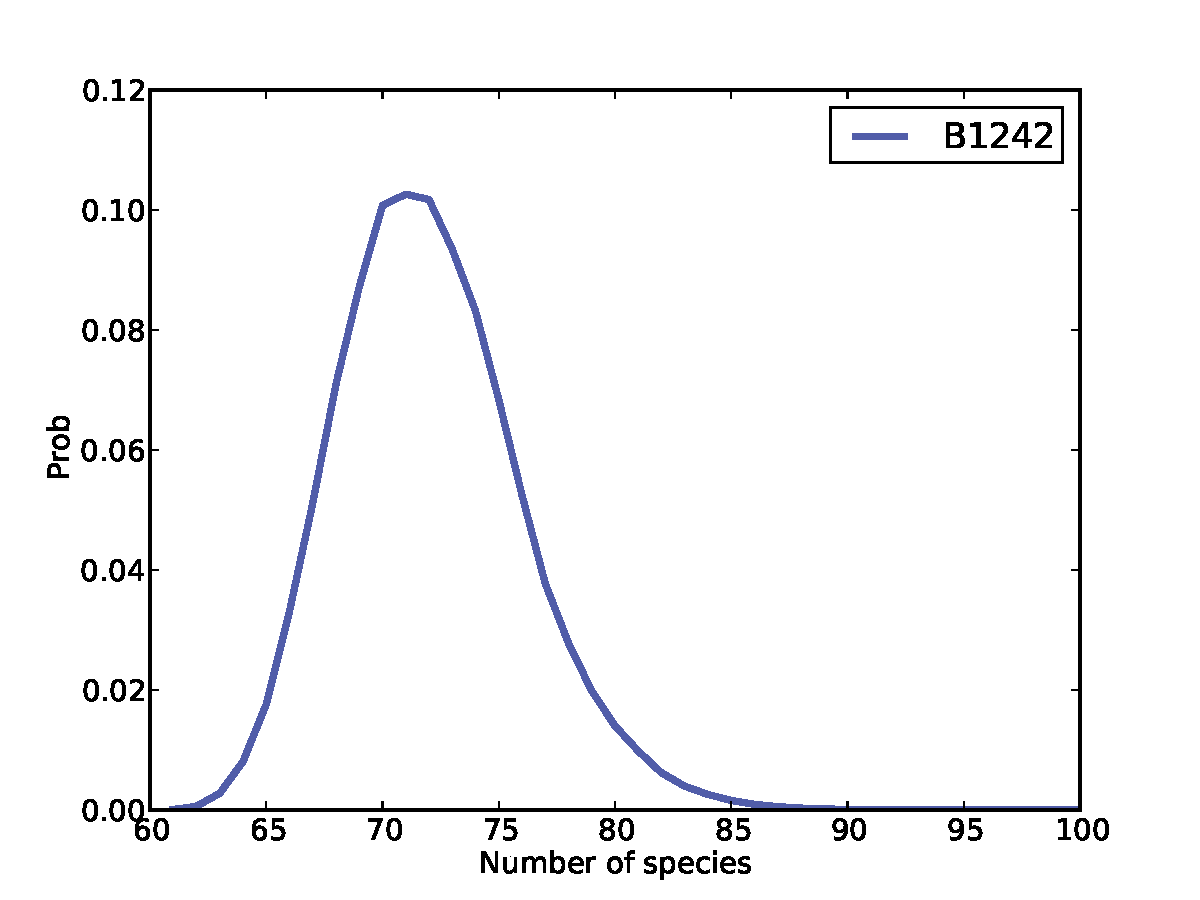
\includegraphics[height=2.5in]{figs/species-ndist-B1242.pdf}}
\caption{Distribution of {\tt n} for subject B1242.}
\label{species-ndist}
\end{figure}

In addition, {\tt Subject.Process} creates a suite, specifically
a suite of type {\tt Species5}, which represents the distribution
of {\tt n} and the prevalences after processing the data.

It also provides {\tt PlotDistOfN}, which plots the posterior
distribution of {\tt n}.  Figure~\ref{species-ndist} shows this
distribution for subject B1242.
The probability that there are exactly 61
species, and no unseen
species, is nearly zero.  The most likely value is 72,
with 90\% credible interval 66 to 79.  At the high end, it is
unlikely that there are as many as 87 species.

Next we compute the posterior distribution of prevalence for
each species.  {\tt Species2} provides {\tt DistOfPrevalence}:

\begin{verbatim}
# class Species2

    def DistOfPrevalence(self, index):
        pmfs = thinkbayes.Pmf()

        for n, prob in zip(self.ns, self.probs):
            beta = self.MarginalBeta(n, index)
            pmf = beta.MakePmf()
            pmfs.Set(pmf, prob)

        mix = thinkbayes.MakeMixture(pmfs)
        return pmfs, mix
\end{verbatim}

{\tt index} indicates which species we want.  For each
value of {\tt n}, we have a different posterior distribution
of prevalence.  

\begin{figure}
% species.py
\centerline{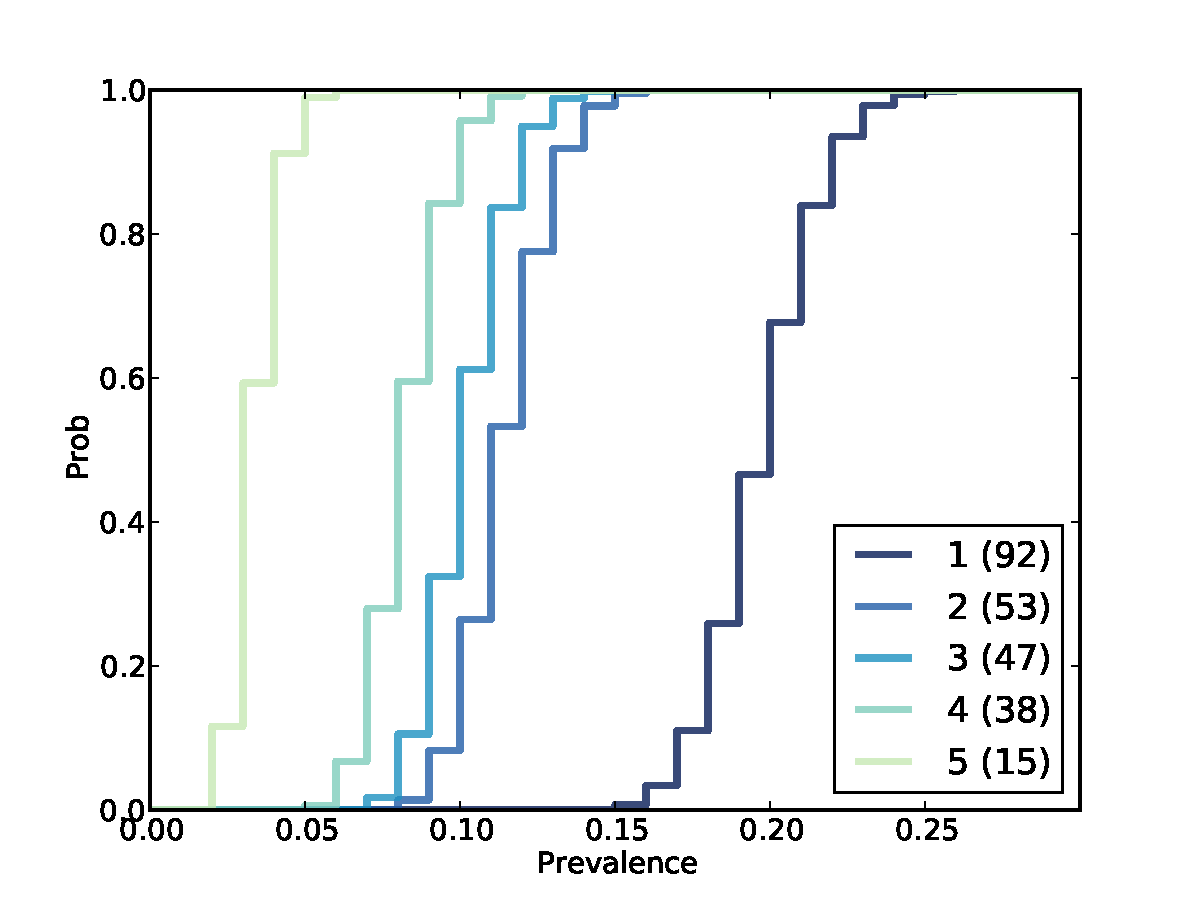
\includegraphics[height=2.5in]{figs/species-prev-B1242.pdf}}
\caption{Distribution of prevalences for subject B1242.}
\label{species-prev}
\end{figure}

So the loop iterates through the possible values of {\tt n}
and their probabilities.  For each value of {\tt n} it gets
a Beta object representing the marginal distribution for the
indicated species.  Remember that Beta objects contain the
parameters {\tt alpha} and {\tt beta}; they don't have
values and probabilities like a Pmf, but they provide {\tt MakePmf}
which generates a discrete approximation to the continuous
beta distribution.

{\tt pmfs} is a MetaPmf that contains the distributions
of prevalence, conditioned on {\tt n}.  {\tt MakeMixture}
combines the MetaPmf into {\tt mix}, which combines the
conditional distributions into the answer, a single distribution
of prevalence.

Figure~\ref{species-prev} shows these distributions for the five
species with the most reads.  The most prevalent species accounts for
23\% of the 400 reads, but since there are almost certainly unseen
species, the most likely estimate for its prevalence is 20\%,
with 90\% credible interval between 17\% and 23\%.

\section{Predictive distributions}

\begin{figure}
% species.py
\centerline{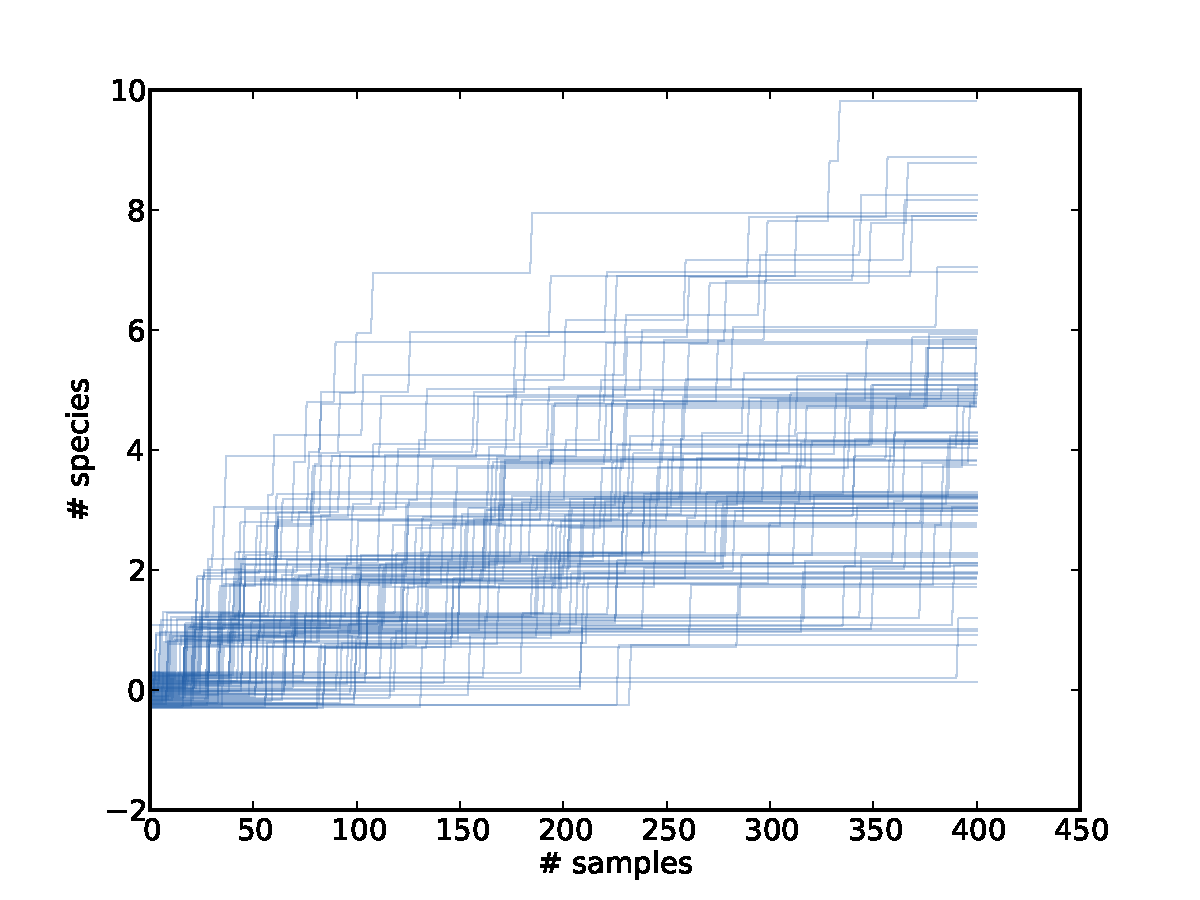
\includegraphics[height=2.5in]{figs/species-rare-B1242.pdf}}
\caption{Simulated rarefaction curves for subject B1242.}
\label{species-rare}
\end{figure}

I introduced the hidden species problem in the form of four related
questions.  We have answered the first two by computing the posterior
distribution for {\tt n} and the prevalence of each species.

The other two questions are:

\begin{itemize}

\item If we are planning to collect additional samples, can we predict
  how many new species we are likely to discover?

\item How many additional reads are needed to increase the
  fraction of observed species to a given threshold?

\end{itemize}

To answer predictive questions like this we can use the posterior
distributions to simulate possible future events and compute
predictive distributions for the number of species, and fraction of
the total, we are likely to see.

The kernel of these simulations looks like this:

\begin{enumerate}

\item Choose {\tt n} from its posterior distribution.

\item Choose a prevalence for each species, including possible unseen
  species, using the Dirichlet distribution.

\item Generate a random sequence of future observations.

\item Compute the number of new species, \verb"num_new", as a function
  of the number of additional samples, {\tt k}.

\item Repeat the previous steps and accumulate the joint distribution
  of \verb"num_new" and {\tt k}.

\end{enumerate}

And here's the code.  {\tt RunSimulation} runs a single simulation:

\begin{verbatim}
# class Subject

    def RunSimulation(self, num_samples):
        m, seen = self.GetSeenSpecies()
        n, observations = self.GenerateObservations(num_samples)

        curve = []
        for k, obs in enumerate(observations):
            seen.add(obs)

            num_new = len(seen) - m
            curve.append((k+1, num_new))

        return curve
\end{verbatim}

\verb"num_samples" is the number of additional samples to simulate.
{\tt m} is the number of seen species, and {\tt seen} is a set of
strings with a unique name for each species.
{\tt n} is a random value from the posterior distribution, and
{\tt observations} is a random sequence of species names.

The result of {\tt RunSimulation} is a ``rarefaction curve'',
represented as a list of pairs with the number of samples and
the number of new species seen.

Before we see the results, let's look at {\tt GetSeenSpecies} and
{\tt GenerateObservations}.

\begin{verbatim}
#class Subject

    def GetSeenSpecies(self):
        names = self.GetNames()
        m = len(names)
        seen = set(SpeciesGenerator(names, m))
        return m, seen
\end{verbatim}

{\tt GetNames} returns the list of species names that appear in
the data files, but for many subjects these names are not unique.
So I use {\tt SpeciesGenerator} to extend each name with a serial
number:

\begin{verbatim}
def SpeciesGenerator(names, num):
    i = 0
    for name in names:
        yield '%s-%d' % (name, i)
        i += 1

    while i < num:
        yield 'unseen-%d' % i
        i += 1
\end{verbatim}

Given a name like {\tt Corynebacterium}, {\tt SpeciesGenerator} yields
{\tt Corynebacterium-1}.  When the list of names is exhausted, it
yields names like {\tt unseen-62}.

Here is {\tt GenerateObservations}:

\begin{verbatim}
# class Subject

    def GenerateObservations(self, num_samples):
        n, prevalences = self.suite.Sample()

        names = self.GetNames()
        name_iter = SpeciesGenerator(names, n)

        d = dict(zip(name_iter, prevalences))
        cdf = thinkbayes.MakeCdfFromDict(d)
        observations = cdf.Sample(num_samples)

        return n, observations
\end{verbatim}

Again, \verb"num_samples" is the number of additional samples
to generate.  {\tt n} and {\tt prevalences} are samples from
the posterior distribution.

{\tt cdf} is a Cdf object that maps species names, including the
unseen, to cumulative probabilities.  Using a Cdf makes it efficient
to generate a random sequence of species names.

Finally, here is {\tt Species2.Sample}:

\begin{verbatim}
    def Sample(self):
        pmf = self.DistOfN()
        n = pmf.Random()
        prevalences = self.SampleConditional(n)
        return n, prevalences
\end{verbatim}

And {\tt SampleConditional}, which generates a sample of
prevalences conditioned on {\tt n}:

\begin{verbatim}
# class Species2

    def SampleConditional(self, n):
        params = self.params[:n]
        gammas = numpy.random.gamma(params)
        gammas /= gammas.sum()
        return gammas
\end{verbatim}

We saw this algorithm for generating prevalences previously
in {\tt Species2.SampleLikelihood}.

Figure~\ref{species-rare} shows 100 simulated rarefaction curves
for subject B1242.  I shifted each curve by a random offset so they
would not all overlap.  By inspection we can estimate that after
400 more samples we are likely to find 2--6 new species.


\section{Joint posterior}

\begin{figure}
% species.py
\centerline{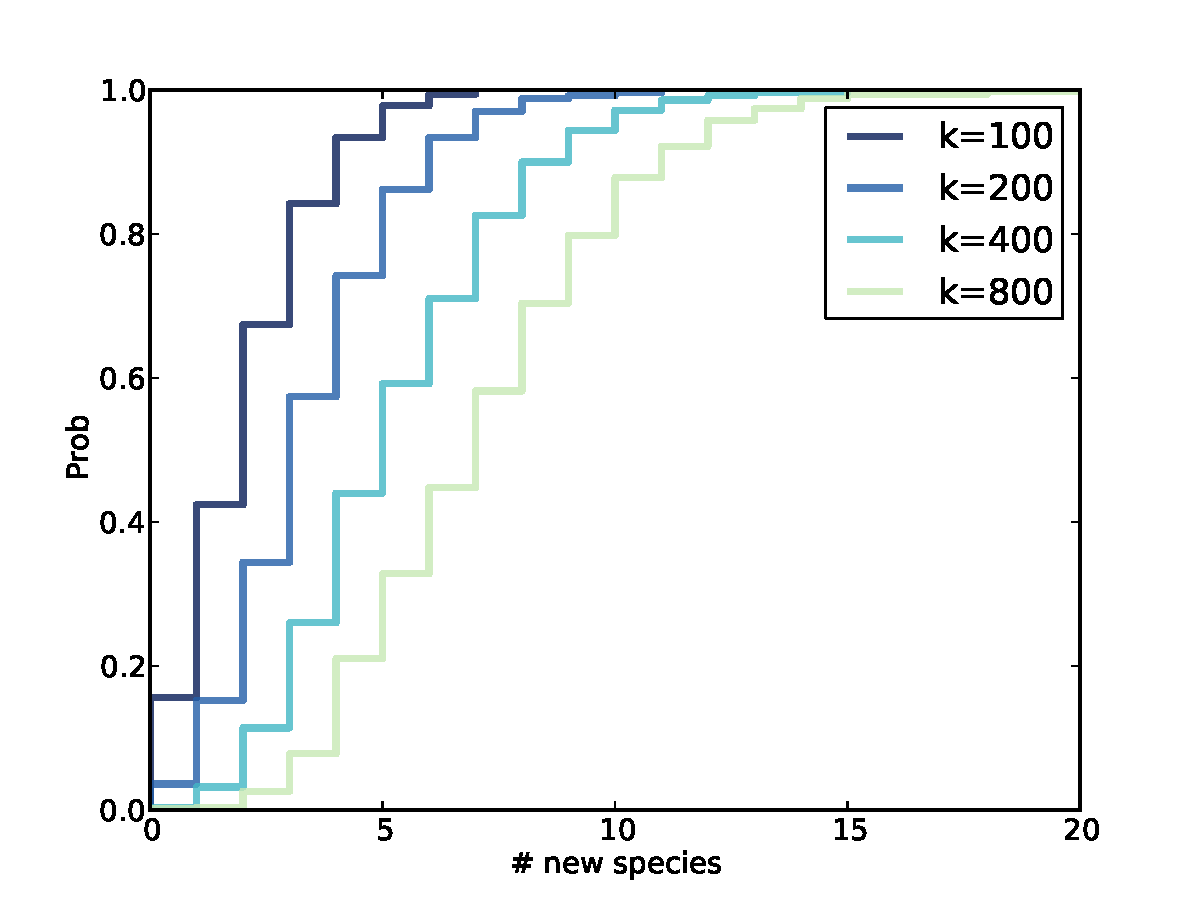
\includegraphics[height=2.5in]{figs/species-cond-B1242.pdf}}
\caption{Distributions of the number of new species conditioned on
the number of additional samples.}
\label{species-cond}
\end{figure}

To be more precise, we can use the simulations to estimate the
joint distribution of \verb"num_new" and {\tt k}, and from that
we can get the distribution of \verb"num_new" conditioned on any
value of {\tt k}.

\begin{verbatim}
# class Subject

    def MakeJointPredictive(self, curves):
        joint = thinkbayes.Joint()
        for curve in curves:
            for k, num_new in curve:
                joint.Incr((k, num_new))
        joint.Normalize()
        return joint
\end{verbatim}

{\tt MakeJointPredictive} makes a Joint object, which is a
{\tt Pmf} whose values are tuples.

{\tt curves} is a list of rarefaction curves created by
{\tt RunSimulation}.  Each curve contains a list of pairs of
{\tt k} and \verb"num_new".

The resulting joint distribution is a map from each pair to
its probability of occurring.  Given the joint distribution, we
can get the distribution of \verb"num_new" conditioned on {\tt k}:

\begin{verbatim}
# class Joint

    def Conditional(self, i, j, val):
        pmf = Pmf()
        for vs, prob in self.Items():
            if vs[j] != val: continue
            pmf.Incr(vs[i], prob)

        pmf.Normalize()
        return pmf
\end{verbatim}

{\tt i} is the index of the variable whose distribution we want;
{\tt j} is the index of the conditional variables, and {\tt val}
is the value the {\tt j}th variable has to have.
You can think of this operation as taking vertical slices out
of Figure~\ref{species-rare}.

{\tt Subject.MakeConditionals} takes a list of {\tt ks}
and computes the conditional distribution of \verb"num_new"
for each {\tt k}.  The result is a list of Cdf objects.

\begin{verbatim}
# class Subject

    def MakeConditionals(self, curves, ks):
        joint = self.MakeJointPredictive(curves)

        cdfs = []
        for k in ks:
            pmf = joint.Conditional(1, 0, k)
            pmf.name = 'k=%d' % k
            cdf = thinkbayes.MakeCdfFromPmf(pmf)
            cdfs.append(cdf)

        return cdfs
\end{verbatim}

Figure~\ref{species-cond} shows the results.  After 100 samples, the
median predicted number of new species is 2; the 90\% credible
interval is 0 to 5.  After 800 samples, we expect to see 3 to 12 new
species.

\section{Coverage}

\begin{figure}
% species.py
\centerline{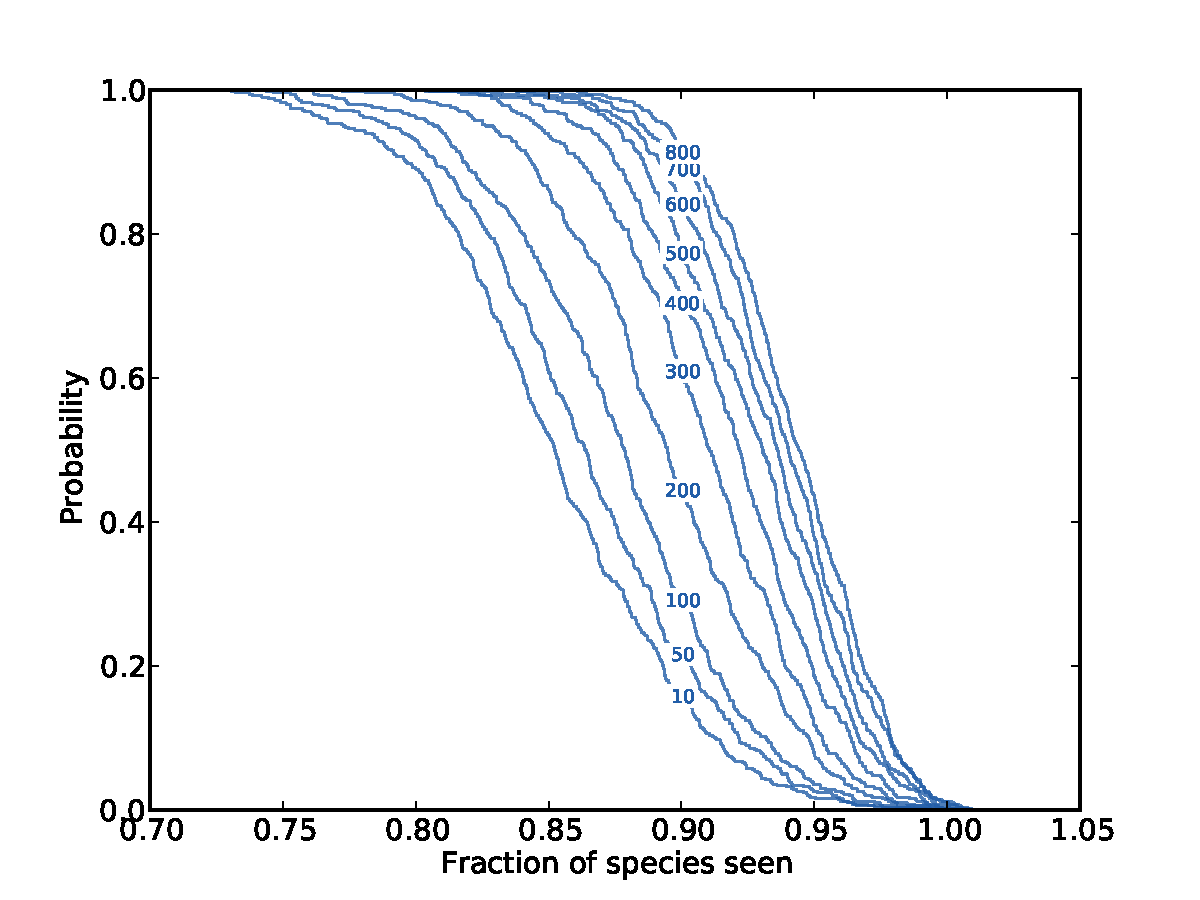
\includegraphics[height=2.5in]{figs/species-frac-B1242.pdf}}
\caption{Complementary CDF of coverage for a range of additional samples.}
\label{species-frac}
\end{figure}

The last question we want to answer is, ``How many additional reads
are needed to increase the fraction of observed species to a given
threshold?''

To answer this question, we'll need a version of {\tt RunSimulation}
that computes the fraction of observed species rather than the
number of new species.

\begin{verbatim}
# class Subject

    def RunSimulation(self, num_samples):
        m, seen = self.GetSeenSpecies()
        n, observations = self.GenerateObservations(num_samples)

        curve = []
        for k, obs in enumerate(observations):
            seen.add(obs)

            frac_seen = len(seen) / float(n)
            curve.append((k+1, frac_seen))

        return curve
\end{verbatim}

Next we loop through each curve and make a dictionary, {\tt d},
that maps from the number of additional samples, {\tt k}, to
a list of {\tt fracs}; that is, a list of values for the
coverage achieved after {\tt k} samples.

\begin{verbatim}
    def MakeFracCdfs(self, curves):
        d = {}
        for curve in curves:
            for k, frac in curve:
                d.setdefault(k, []).append(frac)

        cdfs = {}
        for k, fracs in d.iteritems():
            cdf = thinkbayes.MakeCdfFromList(fracs)
            cdfs[k] = cdf

        return cdfs
\end{verbatim}

Then for each value of {\tt k} we make a Cdf of {\tt fracs}; this Cdf
represents the distribution of coverage after {\tt k} samples.

Remember that the CDF tells you the probability of falling below a
given threshold, so the {\em complementary} CDF tells you the
probability of exceeding it.  Figure~\ref{species-frac} shows
complementary CDFs for a range of values of {\tt k}.

To read this figure, select the level of coverage you want to achieve
along the $x$-axis.  As an example, choose 90\%.

Now you can read up the chart to find the probability of achieving
90\% coverage after {\tt k} samples.  For example, with 300 samples,
you have about a 60\% of getting 90\% coverage.  With 700 samples, you
have a 90\% chance of getting 90\% coverage.

With that, we have answered the four questions that make up the unseen
species problem.  This has been a longer chapter than most, but I
think there is a lot to it.  So if you made it this far,
congratulations!



%\chapter{Future chapters}

%Bayesian regression (hybrid version with resampling?)
%\url{http://www.reddit.com/r/statistics/comments/1647yj/which_regression_technique/}

%Change point detection: 

%Deconvolution: Estimating round trip times

%Bayesian search

%Extension of the Euro problem: evaluating reddit items and redditors
%\url{http://www.reddit.com/r/statistics/comments/15rurz/question_about_continuous_bayesian_inference/}

%Charles Darwin Problem (capture-tag-recapture)
%\url{http://maximum-entropy-blog.blogspot.com/2012/04/capture-recapture-and-charles-darwin.html}

% http://camdp.com/blogs/how-solve-price-rights-showdown

% https://github.com/CamDavidsonPilon/Probabilistic-Programming-and-Bayesian-Methods-for-Hackers

\end{document}
